\documentclass[a4paper,12pt]{report}
\usepackage[T1]{fontenc}
\usepackage[utf8x]{inputenc} 
\usepackage[french]{babel} 
\usepackage{url}
\usepackage{float}
\usepackage{graphicx}
\usepackage[titletoc]{appendix}
\usepackage{a4wide}
\usepackage{listings} 
\usepackage[colorlinks=true,urlcolor=blue,linkcolor=blue]{hyperref}

\frenchbsetup{StandardLists=true}
\renewcommand{\appendixtocname}{Annexes}
\renewcommand{\appendixpagename}{Annexes} 
\addto\captionsfrench{\def\tablename{{Tableau}}}
\newenvironment*{remerciements}{%
\renewcommand*{\abstractname}{Remerciements}
\begin{abstract}
}{\end{abstract}}

\bibliographystyle{alphaurl} 
\begin{document}

\title{Mémoire\\
  \textit{Réalisation d'un jeu d'Othello}
  }

\author{Morgane Badré\\
  Benjamin Letourneau,\\
  Vincent Wilmet,\\
  Nicolas Yvon\\ \\
  Client : M. Zeitoun \\
  Chargé de TD : M. Frey}
\date\today

\maketitle


\begin{remerciements}
\begin{itemize}
  \item M. Narbel, responsable de l’UE PDP pour les cours dispensés.
  \item M. Zeitoun, notre client, qui a pris sur son temps pour effectuer des réunions hebdomadaires et pour nous avoir donné de nombreux conseils.
  \item M. Frey, notre chargé de TD, pour nous avoir aidé et donné des conseils pour le PDP.
  \item M. le rapporteur inconnu qui a contribué de manière anonyme à notre évaluation.
\end{itemize}
\end{remerciements}


\begin{abstract}

L’objectif de ce projet est de réaliser un jeu Othello permettant de jouer Humain opposé à une intelligence artificielle (IA) ou IA contre IA. Une IA est un logiciel qui a pour but de reproduire “intelligemment” un comportement spécifique, ici gagner une partie Othello. Le jeu, avec une interface intuitive, doit permettre à l’utilisateur de pouvoir choisir le niveau (difficulté) de  l’IA en tant qu’aide et joueur.

Le projet s’est déroulé en différentes étapes. Tout d’abord, des recherches ont été effectuées afin de découvrir le jeu et sa communauté, mais également ses spécificités scientifiques. Puis, une analyse des besoins nous a permis de définir clairement les attentes du client. Dans un troisième temps, nous avons mis en place l’architecture du jeu. Le développement a ensuite commencé et pour terminer, une série de tests va être présentée.
\end{abstract}

\begingroup
\hypersetup{linkcolor=black}
\tableofcontents
\endgroup

\hypersetup{linkcolor=blue}

\phantomsection
\chapter*{Introduction}

Le travail que nous présentons dans ce rapport correspond à un projet informatique de programmation que nous avons réalisé en quadrinôme dans le cadre de notre première année de Master informatique de l’Université de Bordeaux.

Le thème de notre projet est de gérer la conduite d’un projet : développer un jeu Othello. Pour cela, nous sommes encadrés par un client (M. Zeitoun) qui nous exprime ses besoins et un chargé de TD (M. Frey) qui nous supervise et nous dirige au fur et à mesure de l’avancement du projet et de ses différentes étapes. Nous bénéficions également des techniques et conseils vuent lors des cours dispensés par M. Narbel.

Les objectifs principaux attendus pour ce projet étaient : de définir les éléments nécessaires pour représenter les différentes configurations du jeu, sur plateaux de taille variable, typiquement 6x6 ou 8x8 cases, de programmer un joueur automatique naïf, suivant une heuristique très simple en début de partie, et explorant tout l'arbre des parties lorsqu'il reste peu de coups à jouer ; et d’utiliser une ou plusieurs heuristiques pour améliorer le joueur naïf (Minimax, Alpha-Beta, ...).

Othello est un jeu de stratégie à deux joueurs : Noir et Blanc. Il se joue sur un plateau unicolore de 64 cases, 8 sur 8 appelé othellier. Ces joueurs disposent de 64 pions bicolores, noirs d’un côté et blancs de l’autre. Le but du jeu est d’avoir plus de pions de sa couleur que l’adversaire à la fin de la partie. Celle-ci s’achève lorsque aucun des deux joueurs n’a de coup légal à jouer. Cela intervient généralement lorsque les 64 cases sont occupées (définition de la Fédération Française d’Othello).

Il a été sujet à de nombreuses utilisations par des scientifiques lors de tournois. Ces rencontres permettaient de mesurer la performance de leur Intelligence Artificielle, les unes par rapport aux autres.

Ainsi ce projet est centré
sur la réalisation du logiciel et plus particulièrement sur une IA compétitive. De plus, les différents besoins de notre client nous ont amenés à réaliser un logiciel Othello amélioré proposant des fonctionnalités supplémentaires au jeu Othello générique.

Notre rapport se décompose en quatre parties dont les premières correspondent aux recherches effectuées avec une étude de l’existant, une bibliographie et une analyse des besoins. Puis, nous présentons notre projet avec nos choix de conception, l’architecture logicielle, les spécificités du jeu, nos choix d’implémentation et les algorithmes utilisés. Enfin, nous évoquerons les fonctionnalités existantes, améliorations que nous pourrions apporter dans le futur ainsi que les différents tests que nous avons réalisés.

\addcontentsline{toc}{chapter}{Introduction}


\chapter{Analyse de l'existant}

\documentclass[a4paper,12pt]{article} 
\usepackage[utf8x]{inputenc} 
\usepackage[french]{babel} 
\usepackage{hyperref}
\usepackage{fullpage}
\usepackage{url}
\usepackage{a4wide}


\bibliographystyle{alphaurl} 
\begin{document}

\title{Étude bibliographique et de l'existant pour le projet\\
  \textit{Réalisation d'un jeu d'Othello}}

\author{Morgane Badré\\
   Benjamin Letourneau,\\
   Vincent Wilmet,\\
   Nicolas Yvon\\}
 \date{}

\maketitle

\section{Éléments bibliographiques} 

\nocite{*}

Pour plus de lisibilité, nous avons partagé notre bibliographie en trois catégories. Une première partie contiendra les généralités sur les jeux d’accessiblité. La deuxième regroupera les algorithmes de force brute : IA basique et la dernière partie présentera les algorithmes évolutionnistes et les réseaux neuraux.


\subsection{Généralités sur les jeux d'accessibilité}

Les jeux d’accessibilité, le plus souvent en tour par tour et entre deux
joueurs, consistent à déplacer des pièces sur un plateau contenant un
nombre fini de positions. Le but étant de capturer les positions du
plateau ou bien les pièces de l'adversaire afin de gagner (Jeu d’échecs, dames,...).

\subsubsection{The evolution of strong othello program}
Cet article \cite{a} est particulièrement intéressant pour notre projet car il présente les meilleurs programmes existant du jeu Othello, par ordre chronologique, en expliquant brièvement les algorithmes/heuristiques utilisés.

\subsubsection{Strategy Guide for Reversi and Reversed Reversi}
Ce site \cite{strategy} explique les différentes règles du jeu ainsi que les heuristiques dans le but de remporter une partie d'Othello (ainsi que d'anti-Othello).

\subsubsection{Site Web : Tothello}
Ce site web \cite{4} présente deux solutions possibles pour une partie d'Othello sur une grille de 6x6, résolue grâce à un logiciel s'appelant Tothello. Il explique aussi les règles de base d'Othello et de l'anti-Othello (“Reversed Othello”).

\subsection{Algorithmes de force-brute et IA basique}

Les algorithmes de force brute permettent de calculer un résultat en
énumérant systéma- tiquement toutes les solutions possibles et vérifiant pour chaque solution si elle satisfait le résultat attendu.

\subsubsection{ProbCut: An Effective Selective Extension of the
  Alpha-Beta Algorithm}
Cet article \cite{5a} décrit l'algorithme ProbCut, une amélioration de
l'algorithme alpha-beta utilisé dans le logiciel LOGISTELLO. Cet
algorithme consiste à couper les sous-arbres inutiles à la recherche
de solution pour une partie.

\subsubsection{How Machines have Learned to Play Othello}
Cet article \cite{5b} est un tour d'horizon des techniques de
résolution des jeux d'accessibilité: fonctions d'évaluations des
positions, recherches sélectives par l'algorithme Multi-ProbCut.

\subsubsection{Improving heuristic mini-max search by supervised learning (2002)}
Cet article \cite{15} présente les algorithmes utilisés pour la
réalisation du logiciel LOGISTELLO II. Il est utile car il explique en
détail le fonctionnement du logiciel (GLEM, ProbCut, ...) et nous
permettra d'améliorer nos propres algorithmes.

\subsubsection{An Analysis of Heuristics in Othello (2004)}
Cet article \cite{13} présente les différents heuristiques utilisables
pour la résolution d'Othello ainsi que les algorithmes alpha-beta et
MiniMax (Component-wise, Coin Parity, Mobility, Stability).

\subsubsection{Site web officiel de la fédération française d'Othello}
Ce site \cite{1} présente les différents algorithmes de recherches
dans les arbres de jeu (Minimax, coupures alpha-beta..) et les
méthodes spécifiques du jeu Othello comme le tri des coups, la
recherche sélective.

\subsubsection{Compte-rendu d'une étude sur le jeu Reversi (1992)}
Les recherches \cite{6} portent sur l'élaboration de la stratégie
gagnante avec une analyse de l'Othello à grille 4x4 (dénombrements sur l'arbre,
heuristique de jeu, explication de plusieurs stratégies possibles) et
de l'Othello à grille 8x8.

\subsubsection{Site Web : Radagast - Othello}
Ce site web \cite{3} présente un logiciel implémentant le jeu Othello
et des conseils sur la réalisation d'un algorithme de résolution du
jeu.

\subsubsection{Experiments with Multi-ProbCut and a new High-Quality Evaluation Function for Othello}
Cet article \cite{8} présente les améliorations apportées
au logicel Logistello, résolvant le jeu Othello. Une
amélioration de la fonction d'évaluation et de l'algorithme
ProbCut, le Multi-ProbCut, sont décrits dans cet article.

\subsubsection{Programmation des échecs et d'autres jeux}
Cet article \cite{7} explique la démarche de résolution des
jeux d'accessibilité par l'utilisation de fonctions
d'évaluation et de l'algorithme MiniMax expliqués au travers
du jeu du pile ou face puis appliquer au jeu d'échecs.

\subsection{Algorithmes évolutionnistes et réseaux neuraux}

Les algorithmes évolutionnistes consistent à faire évoluer un ensemble de solutions par itération d’un nouvel ensemble de solution amélioré. Ils sont utilisés dans le but d’optimiser la résolution de problèmes.
Les réseaux neuraux sont des modèles de calculs basés sur les réseaux de neurones biologiques de l’être humain. Ils sont représentés par des automates.



\subsubsection{Learning of position evaluation in the game of Othello (1995)}
Cet article \cite{b} est intéressant pour nous car il présente une approche
différente de la résolution d'une partie d'Othello. Cette approche
consiste, en partant d'une IA naïve, à arriver à une IA intelligente se
développant en apprenant de ses propres erreurs et des coups du joueur
opposé.

\subsubsection{An Evaluation Function for Othello Based on  Statistics (1997)}
Cet article \cite{c} expose plus en détail le logiciel Logistello II
ainsi que les algorithmes utilisés. Il utilise aussi le principe de
l'auto-apprentissage. 

\subsubsection{Coevolutionary Temporal Difference Learning for Othello (2009)}
Cet article \cite{d} expose deux manières de rendre un programme Othello intelligent et évolutif. Ces deux méthodes sont : “Temporal Difference Learning” (TDL) et “Coevolutionary Learning” (CEL).
Il nous aidera pour améliorer le joueur naïf.

\subsubsection{Strategy acquisition for the game "Othello" based on reinforcement learning}
Cet article \cite{e} explique le fonctionnement d'un nouvel algorithme basé sur le Minimax ainsi que l'auto-apprentissage. Celui-ci nous aidera également pour l'amélioration du joueur naïf.

\subsubsection{Applications of Artificial Intelligence and Machine Learning in Othello (2009)}
Cet article \cite{11} expose une étude basée sur tous les algorithmes
existant (mini-max, alpha-beta, …) ainsi que l'IA évolutive et
effectue des comparaisons.

\subsubsection{Searching for Solutions in Games and Artificial Intelligence (1994)}
Cette thèse \cite{14} présente le principe du jeu résolu et le principe de la
recherche de solution avec une IA. Cette thèse nous sera utile pour
bien appréhender le principe/fonctionnement d'une IA. 


\subsubsection{Site de Fabien Torre, université de Lille, sur l'intelligence artificielle}
Site web \cite{2}  traitant de l'intelligence artificielle et des jeux avec une présentation des algorithmes de jeu comme le Minimax, Alpha-Beta et fonctions d'évaluation. 


\subsubsection{Discovering Complex Othello Strategies Through Evolutionary Neural Networks}
Cet article \cite{9} présente l'utilisation de réseaux neuraux et d'encodage basé sur l'ADN pour la résolution d'Othello.



\section{Étude de l'existant}

Depuis les années 80 \cite{antho} \cite{tour} \cite{otstory}, de nombreux programmes Othello français \cite{prog1} et
étrangers \cite{prog2} ont été créés et se sont défiés lors de tournois afin de
tester leurs performances. Ainsi, nous avons regroupé les programmes
les mieux classés, les plus connus mais aussi des projets autour du
jeu d'Othello.

\subsection{Programmes Othello de renommés}

\subsubsection{Iago}
IAGO \cite{iago} est probablement le premier programme Othello qui ait été créé en 1976 par l'université “Caltech” de Pasadena.
Plusieurs programmes ont porté ce même nom. En effet, en 1982, Paul
Rosembloom de l'université Carnegie-Mellon à Pittsburg (Pennsylvanie)
développe le logiciel IAGO. Ce dernier est plus abouti et plus
performant que la première version. Il est fortement centré sur le
concept de mobilité dont le principe est de capturer les pièces de l'adversaire de façon permanente et limiter les mouvements possibles pour l'adversaire.
Il a utilisé les algorithmes “Current-Mobility”, “Edge-Stability” et “Potential Mobility”.


\subsubsection{Bill}
Il y a eu quatre versions de Bill \cite{bill} dont la première date de 1985 par l'université de Carnegie Mellon et la dernière de 1990 par Kai Fu Lee et Sanjoy Manahan. 
Il est considéré comme un successeur de IAGO car leurs algorithmes sont basés sur le même concept. Sa faculté de prévision des coups suivants lui a permis de vaincre IAGO en un contre un (Inférence bayésienne).
Cette faculté est basée sur des tables contenant les combinaisons  à suivre pour une partie gagnante (killer table).

\subsubsection{Keyano}
Ce programme \cite{keyano} a été écrit par Mark Brockington pendant ses recherches de doctorat en 1996. Pendant les années suivantes, il a fait parti des meilleurs programmes au monde. 
Il utilise essentiellement l'algorithme ProbCut ainsi qu'une IA évolutive gérant une base de données qui contient les jeux de combinaisons possibles.  


\subsubsection{Logistello I}
Ce programme \cite{logistello} a été créé par Michael
Buro en 1991. Il a remporté son premier tournoi en partageant la
première place avec STELLA en Octobre 1993 en Allemagne et en battant KEYANO,  REV (renommé KITTY en 1994), NICKSREV, VERS2 et CHIGOREV. Il domine toutes les IA d'Othello jusqu'en 1996 lorsqu'il a été battu par HANNIBAL.

\subsubsection{Logistello II}
LOGISTELLO II \cite{logistello} est une évolution de Logistello I créé par Michael Buro. Il est considéré comme l'une des meilleurs IA d'Othello. Il a été le premier logiciel à battre le champion du monde Takeshi Mukarami (japonais) en 1997. En 1998, LOGISTELLO arrête les tournois.


\subsubsection{Hannibal}
HANNIBAL, par Martin Piotte et Louis Geoffroy, est un programme d'apprentissage d'Othello écrit en 1996. D'après les résultats des tournois en 1997, il aurait été à peu près aussi fort que LOGISTELLO II à ce moment là. Depuis que LOGISTELLO I a arrêté en 1998, HANNIBAL était certainement le programme actif le plus fort à la fin des années 90. HANNIBAL utilise l'algorithme Minimax et une fonction d'évaluation neurale.

\subsubsection{Zebra}
ZEBRA \cite{3} est un programme implémentant Othello en utilisant
l'algorithme Multi-ProbCut et NegaScout. Il a été créé
en 1997 et a été amélioré jusqu'en 2001. Il a été plusieurs fois en 3ème place lors de tournois.

\subsubsection{Edax}
EDAX est un programme \cite{edax} implémentant une intelligence artificelle pour Othello en utilisant les ressources des machines actuelles, CPU 64-bits et multi-coeur. Il a été créé en 1998 et a été régulièrement amélioré depuis.

\subsubsection{Cyrano}
CYRANO \cite{cyrano} est une applet implémentant une version améliorée de l'algorithme Alpha-Beta, le NegaScout. La dernière version de CYRANO date de 2005.

\subsection{Projets autour d'Othello}

\subsubsection{Projet JACOTHELLON}
A l'université de Montpellier, en deuxième année d'IUT Informatique,
un binôme composé de Audrey Colbrant – Elodie Nouguier, a développé un
jeu nommé Jacothellon \cite{jacothellon}. 
Le projet avait pour but de développer un logiciel mettant en scène deux joueurs : soit deux humains jouant l'un contre l'autre, soit un humain contre une intelligence artificielle à travers le jeu Othello. Le jeu a été développé en Java et sous Eclipse.
Ce rapport nous permet d'avoir une base et une vue d'ensemble sur les
étapes et les difficultés du développement d'un tel jeu.

\subsubsection{Projet jeu d'Othello en java}
Guillaume Sauveur, à l'école d'ingénieur en informatique l'EnsiCaen, a
réalisé un projet en trinôme en java : Othello
\cite{projothello1}. Nous avons à disposition leur compte-rendu
présentant le déroulement du projet notamment avec une partie
portant sur l'intelligence artificielle avec différents niveaux de
difficultés. L'algorithme Minimax, les coupures alpha-bêta et
la fonction d'évaluation sont utilisés pour développer l'IA.


\subsubsection{Projet : Othello en C++ et SFML}
Un rédacteur de tutoriels, Pierre-Emmanuel Mercier, a mis à
disposition sur son site Ace-Art le jeu Othello \cite{projothello2} qu'il a développé avec Alexis Bouvot qui a intégré l'IA.  
Il fournit dans une archive un diagramme de classes UML, le code source en C++ avec la librairie SMFL. 
Le diagramme et le code vont nous être utiles pour avoir une idée globale du travail à réaliser.
 



\bibliography{biblio} 

\end{document}

\chapter{Analyse des besoins}

\documentclass[a4paper,12pt]{article} 
\usepackage[utf8x]{inputenc} 
\usepackage[french]{babel} 
\usepackage[colorlinks=true,urlcolor=blue,linkcolor=blue]{hyperref}
\usepackage{fullpage}
\usepackage{url}
\usepackage{a4wide}
\usepackage{graphicx}
\usepackage{float}
\usepackage[toc,page]{appendix}

\renewcommand{\appendixtocname}{Annexes}
\renewcommand{\appendixpagename}{Annexes} 
\addto\captionsfrench{\def\tablename{{Tableau}}}
\begin{document}

\title{Analyse des besoins et tests pour le projet\\
  \textit{Réalisation d'un jeu d'Othello}}

\author{Morgane Badré\\
  Benjamin Letourneau,\\
  Vincent Wilmet,\\
  Nicolas Yvon\\}
\date{}

\maketitle

Ce document présente l'analyse des besoins pour le projet de Réalisation d'un jeu d'Othello. Deux types de besoins seront étudiés:

\section{Besoins fonctionnels}

Les besoins fonctionnels sont des besoins en rapport direct avec les
demandes de l'utilisateur. Des diagrammes UML accompagnent ces
spécifications afin de simplifier l'analyse (annexes \ref{A}, \ref{B},
\ref{C}). Les fonctionnalités sont classées par priorité de développement.

\subsection{Jouer une partie / mettre en pause une partie}
L’utilisateur doit pouvoir lancer à tout moment une partie avec l'affichage d'un plateau contenant l’environnement initial, ainsi que faire une pause dans le déroulement de la partie. Le lancement d'une partie ne doit pas prendre plus de 2 secondes. Cette fonctionnalité ne sera pas difficile à implémenter.

\begin{description}
\item[Test système] Appuyer sur le bouton lance bien le mode Jeu du logiciel.
\end{description}

\subsection{Réaliser une Intelligence Artificielle (IA) }
\label{IA}
L'utilisateur doit pouvoir jouer contre une Intelligence Artificielle tout d'abord naïve puis plus tard, si possible, évolutive. L'IA doit pouvoir apporter une solution en un temps imparti par l'utilisateur. Le risque de cette approche est que l'IA peut être très longue à répondre selon l'avancée de la partie. Dans ce cas, l'algorithme le plus adapté sera choisi et un compteur de temps sera ajouté pour empêcher tout débordement sur le temps maximal. Cette fonctionnalité est certainement la plus difficile du projet.

\begin{description}
\item[Test comportemental] Vérifier que le résultat de la réflexion de l’IA est correct.
\item[Test de performance] Exécuter le logiciel en même temps qu’un autre (gourmand en ressources) afin de voir si les résultats obtenus sont identiques sur une même partie. (savoir si l’IA est compétente).
\end{description}

\subsection{Enregistrer une partie / Relancer une partie}
L'utilisateur doit pouvoir enregistrer sa partie et la relancer pour pouvoir la continuer. Cette action est réalisée à travers l’actionnement d’un bouton. Le fichier de sauvegarde doit être créé en moins de 5 secondes et ne doit pas dépasser une taille de 10 Ko. Il sera nécessaire d'implémenter un petit analyseur syntaxique et lexical pour la lecture et l'écriture des fichiers de sauvegarde. Les risques de cette fonctionnalité sont qu'il est possible que la sauvegarde soit interrompue et donc qu'il y ait une perte de données, le fichier étant alors corrompu. Ce risque peut être paré par une protection des données du fichier par l'utilisation de balises ouvrantes et fermantes afin de vérifier l'intégrité des données du fichier. Cette fonctionnalité sera facile à implémenter.

\begin{description}
\item[Test système] Le fichier de sauvegarde est bien créé et valide. Le plateau affiché correspond bien au fichier en entrée.
\item[Test aléatoire] Lancer aléatoirement des enregistrements de la partie.
\end{description}

\subsection{Recommencer une partie à une certaine position}
L’utilisateur doit pouvoir recommencer à jouer à une partie, préalablement lancée et enregistrée, en ayant la possibilité de choisir à partir de quel état du plateau recommencer. C’est-à-dire que si 10 coups ont été joués alors l’utilisateur peut choisir de recommencer à partir du deuxième ou bien du huitième. Ainsi, le fichier de sauvegarde doit contenir un historique complet de la partie en l'état. Le temps de chargement d'un fichier de sauvegarde et la mise en place du plateau à la position souhaitée ne doit pas prendre plus de 10 secondes. En cas de crash de la sauvegarde, le système récupèrera l'avant-dernière sauvegarde. Celle-ci a une difficulté d'implémentation normale.

\begin{description}
\item[Test unitaire] La position choisie correspond bien à celle sauvegardée.
\item[Test négatif] Choisir une position hors des bornes de la partie ($<$ 0 ou $>$ au dernier coup).
\end{description}

\subsection{Possibilité de revenir un coup en arrière}

L’utilisateur doit pouvoir, s’il a effectué un déplacement non désiré, revenir en arrière dans le jeu afin de rejouer les coups qu’il désire (mécanisme Défaire/Refaire). L'utilisateur aura le choix parmi tous les coups qu'il avait joués et pourra ainsi revenir en arrière pour tester une stratégie différente. Le temps de modification de l'affichage et de la structure doit être quasi-instantané, une demi-seconde. Une corruption éventuelle d'historique conduit à utiliser l'historique du coup précédent. Il faudra donc garder en mémoire tous les coups joués et permettre de ``revenir en avant'', c'est-à-dire, annuler un retour en arrière. Cette fonctionnalité a une difficulté d'implémentation normale.

\begin{description}
\item[Test unitaire] La position choisie correspond bien à celle sauvegardée.
\item[Test aux limites] Cette fonctionnalité doit être désactivée lorsque qu’il n’y a plus aucun coup précédant le coup actuel.
\item[Test aléatoire] Simulation d'un nombre aléatoire de retours en arrière.
\end{description}

\subsection{Fournir le manuel utilisateur du jeu (interface et règles)}

L'utilisateur doit pouvoir accéder à une aide générale sur le fonctionnement et les règles du jeu. Cette aide sera introduite par l’ouverture d’un fichier PDF qui pèsera moins de 10 Mo. L'explication sera lisible et assimilable en moins de 10-15 minutes. Il faudra alors résumer pour mettre l'essentiel et vulgariser les explications afin qu'elle soit compréhensible par tous. Cette fonctionnalité sera facile à réaliser.

\begin{description}
\item[Test unitaire] Le PDF de l’aide s’affiche bien lors de l’appui sur le bouton.
\end{description}

\subsection{Proposer des suggestions de coups par l'IA}

L’utilisateur doit pouvoir demander au logiciel de l’aide pour visualiser le meilleur coup à jouer après analyse par l’IA qui proposera plusieurs niveaux d'aide comme par exemple, le choix entre les deux meilleurs coups à jouer. L'IA doit répondre en un temps acceptable dans l'ordre de 2 à 3 secondes. L'algorithme utilisé dépendra de l'avancement de la partie. Pour que l'algorithme choisi ne prenne pas trop de temps, on ajoutera un compteur de temps. La difficulté de cette fonctionnalité dépendra de la difficulté de l'intégration de l'IA (voir fonctionnalité n°\ref{IA}).

\begin{description}
\item[Test unitaire] Cette fonctionnalité doit toujours nous renvoyer une position correspondant à un coup valide.
\item[Test aux limites] Ce bouton n'est activé que lorsque le joueur peut jouer.
\end{description}

\subsection{Chargement d’un fichier pré-configuré}

L’utilisateur doit pouvoir sélectionner un fichier qu’il a composé afin de jouer sur un plateau de sa configuration. Ce fichier doit être écrit de façon interprétable par le logiciel. Le fichier doit être vérifié et chargé puis le plateau qui en résulte doit être affiché en 5 secondes maximum. Le fichier peut-être corrumpu donc une vérification de jalons de début et de fin obligatoire ainsi que la présence des informations requises permettra de parer à ce risque. S'il y a corruption du fichier ou une erreur lors de la position des jetons dans le fichier, un message d'erreur s'affichera. Cette fonctionnalité n'est pas dure à implémenter.

\begin{description}
\item[Test système] Le plateau correspond bien au fichier entré si celui-ci est valide.
\end{description}

\subsection{Possibilité de choisir la taille de la grille de jeu}

L'utilisateur doit pouvoir choisir la taille de sa grille de jeu. C'est-à-dire une grille 5*5, 6*6, ... Ou plus. Mais aussi 6*10, ou autre grille rectangulaire. La grille pourra être choisie dans une limite d'au minimum 3x3 jusqu'au maximum 50x50. Le risque de cette fonctionnalité est que l'utilisateur choisisse une grille trop grande ou trop petite pour que le logiciel soit jouable. Il suffira de limiter la taille de la grille et d'obliger l'utilisateur à entrer les bonnes dimensions. Cette fonctionnalité est simple à implémenter.

\begin{description}
\item[Test unitaire] La grille doit correspondre à la taille demandée.
\item[Test négatif] La grille ne doit pas être acceptée si la taille demandée est trop grande ou trop petite.
\item[Test aléatoire] Lancer différentes configurations de grilles qui soient dans l’intervalle autorisé.
\end{description}

\subsection{Menu pour choisir le temps de réflexion de l’IA}

Le joueur doit pouvoir choisir si l’IA prendra plus ou moins beaucoup de temps pour le calcul des coups. Ce temps ne devra pas pouvoir dépasser 2 jours. Cette fonctionnalité ne devrait pas poser de problème particulier.

\begin{description}
\item[Test système] Le temps de réflexion de l’IA doit correspondre à celui donner dans le menu de la partie.
\item[Test aléatoire]  Entrer des temps aléatoires raisonnables, < 3 secondes, pour le temps de réflexion de l’IA et vérifier que l’algorithme le respecte.
\end{description}


\subsection{Possibilité d’échanger les joueurs}

Le logiciel doit permettre au joueur d’échanger sa place avec l’IA et de pouvoir continuer la partie ainsi. Le temps de réponse du logiciel pour échanger les joueurs ne doit pas dépasser plus de 2 secondes. Il ne sera possible d'échanger les joueurs que lorsque la partie aura été commencée et non terminée. Cette fonctionnalité n'est pas dure à implémenter.

\begin{description}
\item[Test unitaire] Il est visuellement possible de voir que nos jetons sont échangés avec ceux de notre adversaire.
\item[Test aléatoire] Tester pendant une partie l’échange des joueurs à des intervalles aléatoires.
\end{description}

\section{Besoins non fonctionnels}

Les besoins non fonctionnels sont des besoins en rapport direct avec le comportement du logiciel et la gestion du projet.

\subsection{Besoins comportementaux}

\subsubsection{Performances}

Le logiciel doit pouvoir s'exécuter en 2-3 secondes maximum. L'algorithme force-brute (recherche exhaustive) doit pouvoir calculer une stratégie maximale de 4x4 en 15 minutes maximum (moyenne). Le temps de calcul de l'algorithme force-brute pour une grille 6x6 ou 8x8 étant considérablement plus élevé, l'utilisation d'algorithmes plus évolués devra être étudiée et expérimentée. Le logiciel ne doit pas dépasser une utilisation de la mémoire supérieure à 2Go.

\begin{description}
\item[Test système] Exécuter le logiciel sur différents types de machines de puissances différentes : petites machines (netBook, notebook), machines de bureau (PC de salon, PC portable moyen, c’est-à-dire avec un dual core + 4go de ram maxi), machines de jeu (Core i7, 16GO de ram, …).
\end{description}

\subsubsection{Fiabilité}

Le logiciel doit implémenter des sauvegardes régulières pour permettre à l’utilisateur de pouvoir reprendre une partie coupée. Ces sauvegardes doivent être intègres.
Le logiciel doit enregistrer au fur et à mesure les coups joués en tant que position (i,j) dans un fichier annexe afin de garder une trace des parties réalisées.
Afin de permettre à l’utilisateur de récupérer une partie en cours avant un crash quelconque de l’ordinateur ou une fermeture de l’application, la partie doit être régulièrement enregistrée afin de pouvoir être relancée.

\begin{description}
\item[Test système] Fermer l’application en plein milieu d’une partie, pendant le chargement d’une partie, pendant la réflexion de l’IA. 
\item[Test aléatoire] Ouvrir les fichiers de sauvegarde afin de vérifier qu’ils ne soient pas corrompus et intègres.
\end{description}

\subsubsection{Facilité d’utilisation}

L’interface graphique sera composée de menus, de boutons et d'une
grille représentant le plateau de jeu (figure \ref{plateau} de
l'annexe \ref{D}). Elle sera simple et intuitive
(autres prototypes de l'interface dans l'annexe \ref{D}).
 
\begin{description}
\item[Test d’utilisation] Faire jouer des personnes inconnues au projet, des personnes ne connaissant pas les règles du jeu Othello, des enfants aux personnes âgées. 
\end{description}

\subsubsection{Domaine d’action}

Il y a deux sortes d’utilisateurs qui seront concernées par le jeu :
\begin{itemize}
\item l'utilisateur ``tout public'', qui a pour but de simplement jouer au jeu.
\item l’utilisateur chercheur / développeur qui sera intéressé pour tester l’efficacité de l’IA, trouver des stratégies gagnantes.
\end{itemize}
Le logiciel peut prendre des fichiers en paramètre qui permettront de commencer une partie sauvegardée ou de créer une situation initiale différente. Un fichier en sortie sera créé à la suite d’une partie remportée pour récupérer l'historique.

\begin{description}
\item[Test d’utilisation] Complément du test de Facilité d’utilisation. Faire jouer des scientifiques pouvant utiliser les résultats du programme à des fins professionnelles.
\end{description}

\subsubsection{Portabilité}

Le logiciel sera fonctionnel pour les plates-formes supportant Java permettant une portabilité sur les machines Unix et Windows.

\begin{description}
\item[Test système] Ce test se fait en complément du test de performance, tester le logiciel sur différents types de machines supportant la JVM (Windows, Mac Os, Linux).
\end{description}

\subsection{Besoins Organisationnels}

\subsubsection{Standards et processus de développement}

\begin{description}
\item[Méthode d’organisation :]
Une réunion par semaine avec le client ainsi qu'une réunion hebdomadaire avec le chargé de TD (en concordance avec le planning imposé par le responsable PdP).
Nous avons prévu des créneaux horaires pour travailler en groupe en plus du travail personnel effectué par chacun.

\item[Outils de spécification :]
On utilise Google Drive pour stocker les rapports des différentes réunions, pour la rédaction commune des documents demandés, Latex pour la mise en page et SVN + Github qui servira de dépôt pour les fichiers sources. 
Nous avons prévu de créer une documentation javadoc et un manuel utilisateur. 

\item [Environnements et systèmes d’exploitation :]
Les systèmes d’exploitation qui seront utilisés pendant le développement sont : Windows, Linux et Mac. Le logiciel sera développé en Java 1.7 avec l’IDE Eclipse. Développer sur différents environnements nous permettra d'effectuer des tests constants sur la portabilité du logiciel.

\end{description}

\subsubsection{Gestion du temps}

Nous avons décidé de représenter notre gestion du temps de travail
grâce à un diagramme de Gantt (figure \ref{diag-gantt}) et un tableau
descriptif de nos tâches (tableau \ref{tab}).

\begin{figure}[H]
  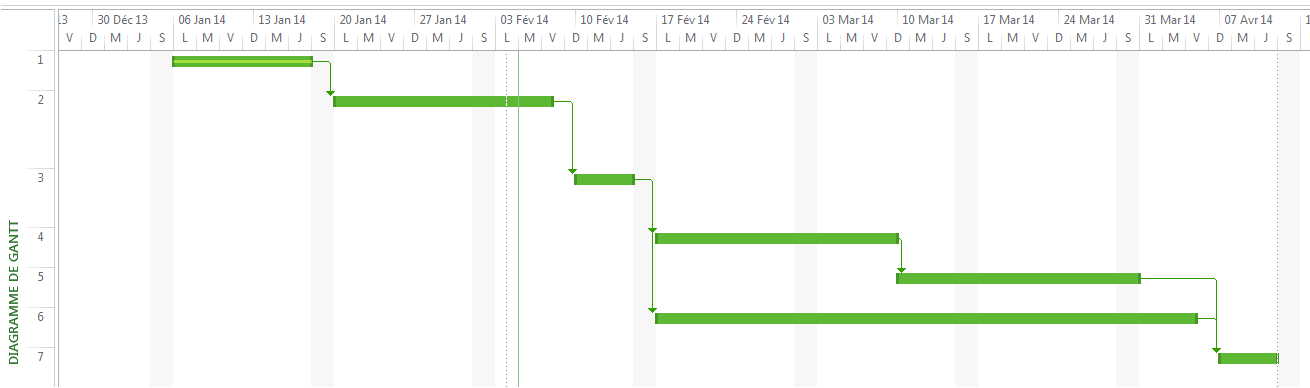
\includegraphics[scale=0.5]{gantt.png}
  \caption{Diagramme de GANTT représentant la gestion du temps pour le projet.}
  \label{diag-gantt}
\end{figure}

\begin{table}[H]
  \resizebox{0.7\textwidth}{2cm}{\begin{minipage}{\textwidth}
      \begin{tabular}{|c|c|c|c|c|c|}
        \hline
        Numéro de Tâche & Nom de la tâche & Durée & Début & Fin & Prédécesseurs \tabularnewline
        \hline
        1 & Bibliographie + Analyse de l'existant & 10 jours & Lun 06/01/14 & Ven 17/01/14 &  \tabularnewline
        \hline
        2 & Rédaction du Cahier des Besoins + Etablissement des Tests & 15 jours & Lun 20/01/14 & Ven 07/02/14 & 1 \tabularnewline
        \hline
        3 & Mise en place de l'architecture Logicielle & 5 jours & Lun 10/02/14 & Ven 14/02/14 & 2 \tabularnewline
        \hline
        4 & Mise en place de l'architecture Logicielle & 5 jours & Lun 10/02/14 & Ven 14/02/14 & 2 \tabularnewline
        \hline
        5 & Mise en place de l'architecture Logicielle & 5 jours & Lun 10/02/14 & Ven 14/02/14 & 2 \tabularnewline
        \hline
        6 & Rédaction du mémoire de projet & 35 jours & Lun 17/02/14 & Ven 04/04/14 & 3 \tabularnewline
        \hline
        7 & Préparation et entraînement pour la soutenance & 5 jours & Lun 07/04/14 & Ven 11/04/14 & 5;6  \tabularnewline
        \hline
      \end{tabular}
      \caption{\label{tab}Tableau descriptif des tâches}
    \end{minipage}}
\end{table}

\begin{enumerate}
\item L'analyse de l'existant permet de commencer le projet, et de réaliser une ébauche de la bibliographie qui sera complétée (modifiée) lors de la rédaction du mémoire final de projet.
\item Rédaction du cahier des Besoins (Fonctionnels et Non-fonctionnels). Etablissement des tests à réaliser pendant et après la phase de développement.
\item Réalisation de l'architecture logicielle. Modélisation à l'aide du logiciel UML Designer.
\item Le développement logiciel contient les tâches suivantes :
  \begin{itemize}
  \item Réalisation de l'IHM 
  \item Réalisation de la gestion des fichiers (pour la sauvegarde d'une partie)
  \item Réalisation de l'Intelligence Artificielle du jeu
  \end{itemize}
  Durant toute la durée de développement logiciel, les tests sont réalisés.
\item Réalisation des tests sur le logiciel afin de traquer les bugs existants.
\item La rédaction du mémoire de projet est répartie sur la durée du développement et des tests. La durée estimée est d'une semaine pour les quatre membres du projet.
\item  Cette partie du projet consiste à la réalisation d'un support de présentation (Power Point). Nous allons aussi réaliser des entraînements de soutenance.
\end{enumerate}

\subsection{Besoins Externes}

\subsubsection{Contraintes d'interopérabilité}

Aucune contrainte.

\subsubsection{Contraintes légales}

Aucune contrainte.

\subsubsection{Contraintes éthiques}

L'IA ne doit pas pouvoir gagner 5 parties de suite.

\appendix
\appendixpage
\addappheadtotoc 

\section{Diagramme de déploiement}
\label{A}
\begin{figure}[H]
  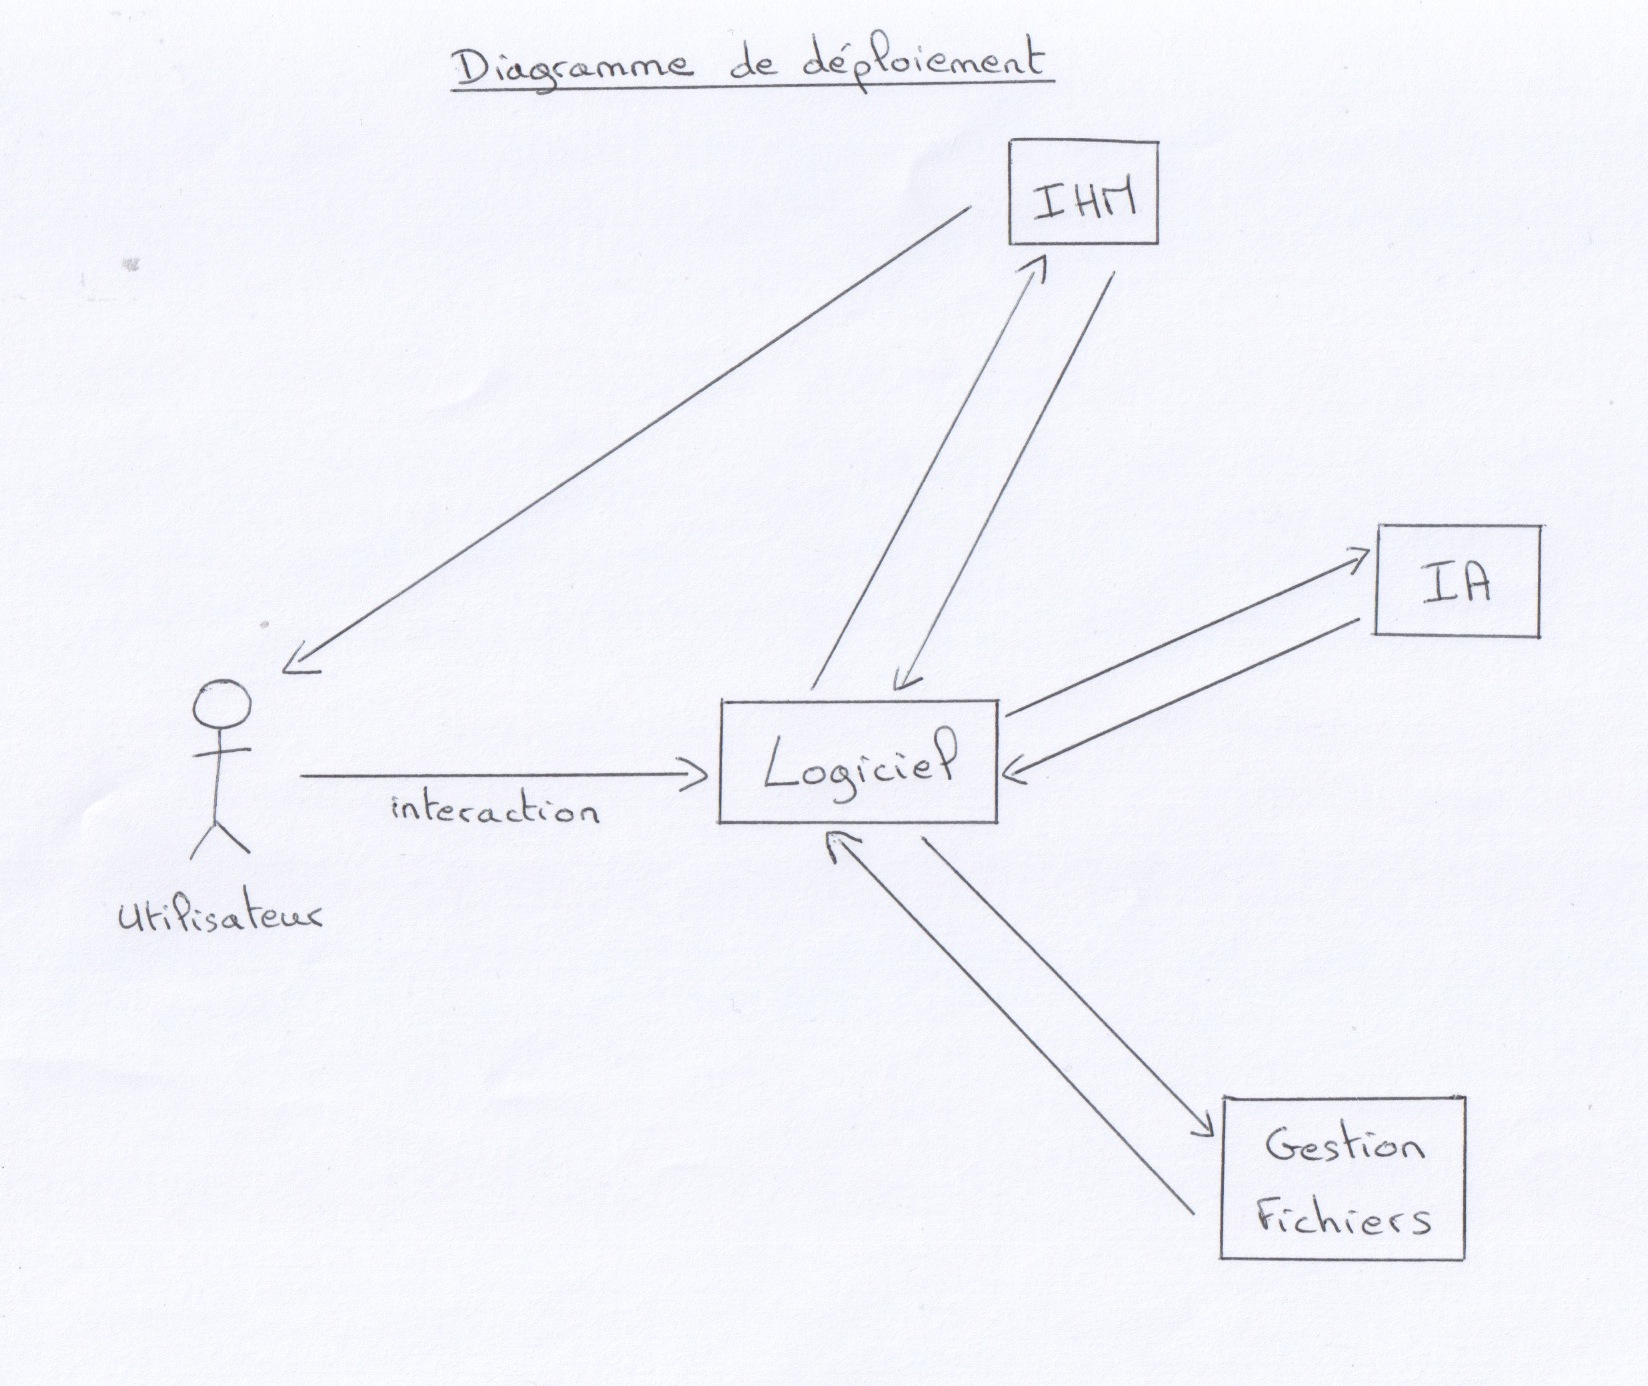
\includegraphics[scale=0.8]{deploiement.jpeg}
\caption{Diagramme UML de déploiement}
\label{deploi}
\end{figure}

\section{Diagramme des cas d'utilisation}
\label{B}
\begin{figure}[H]
  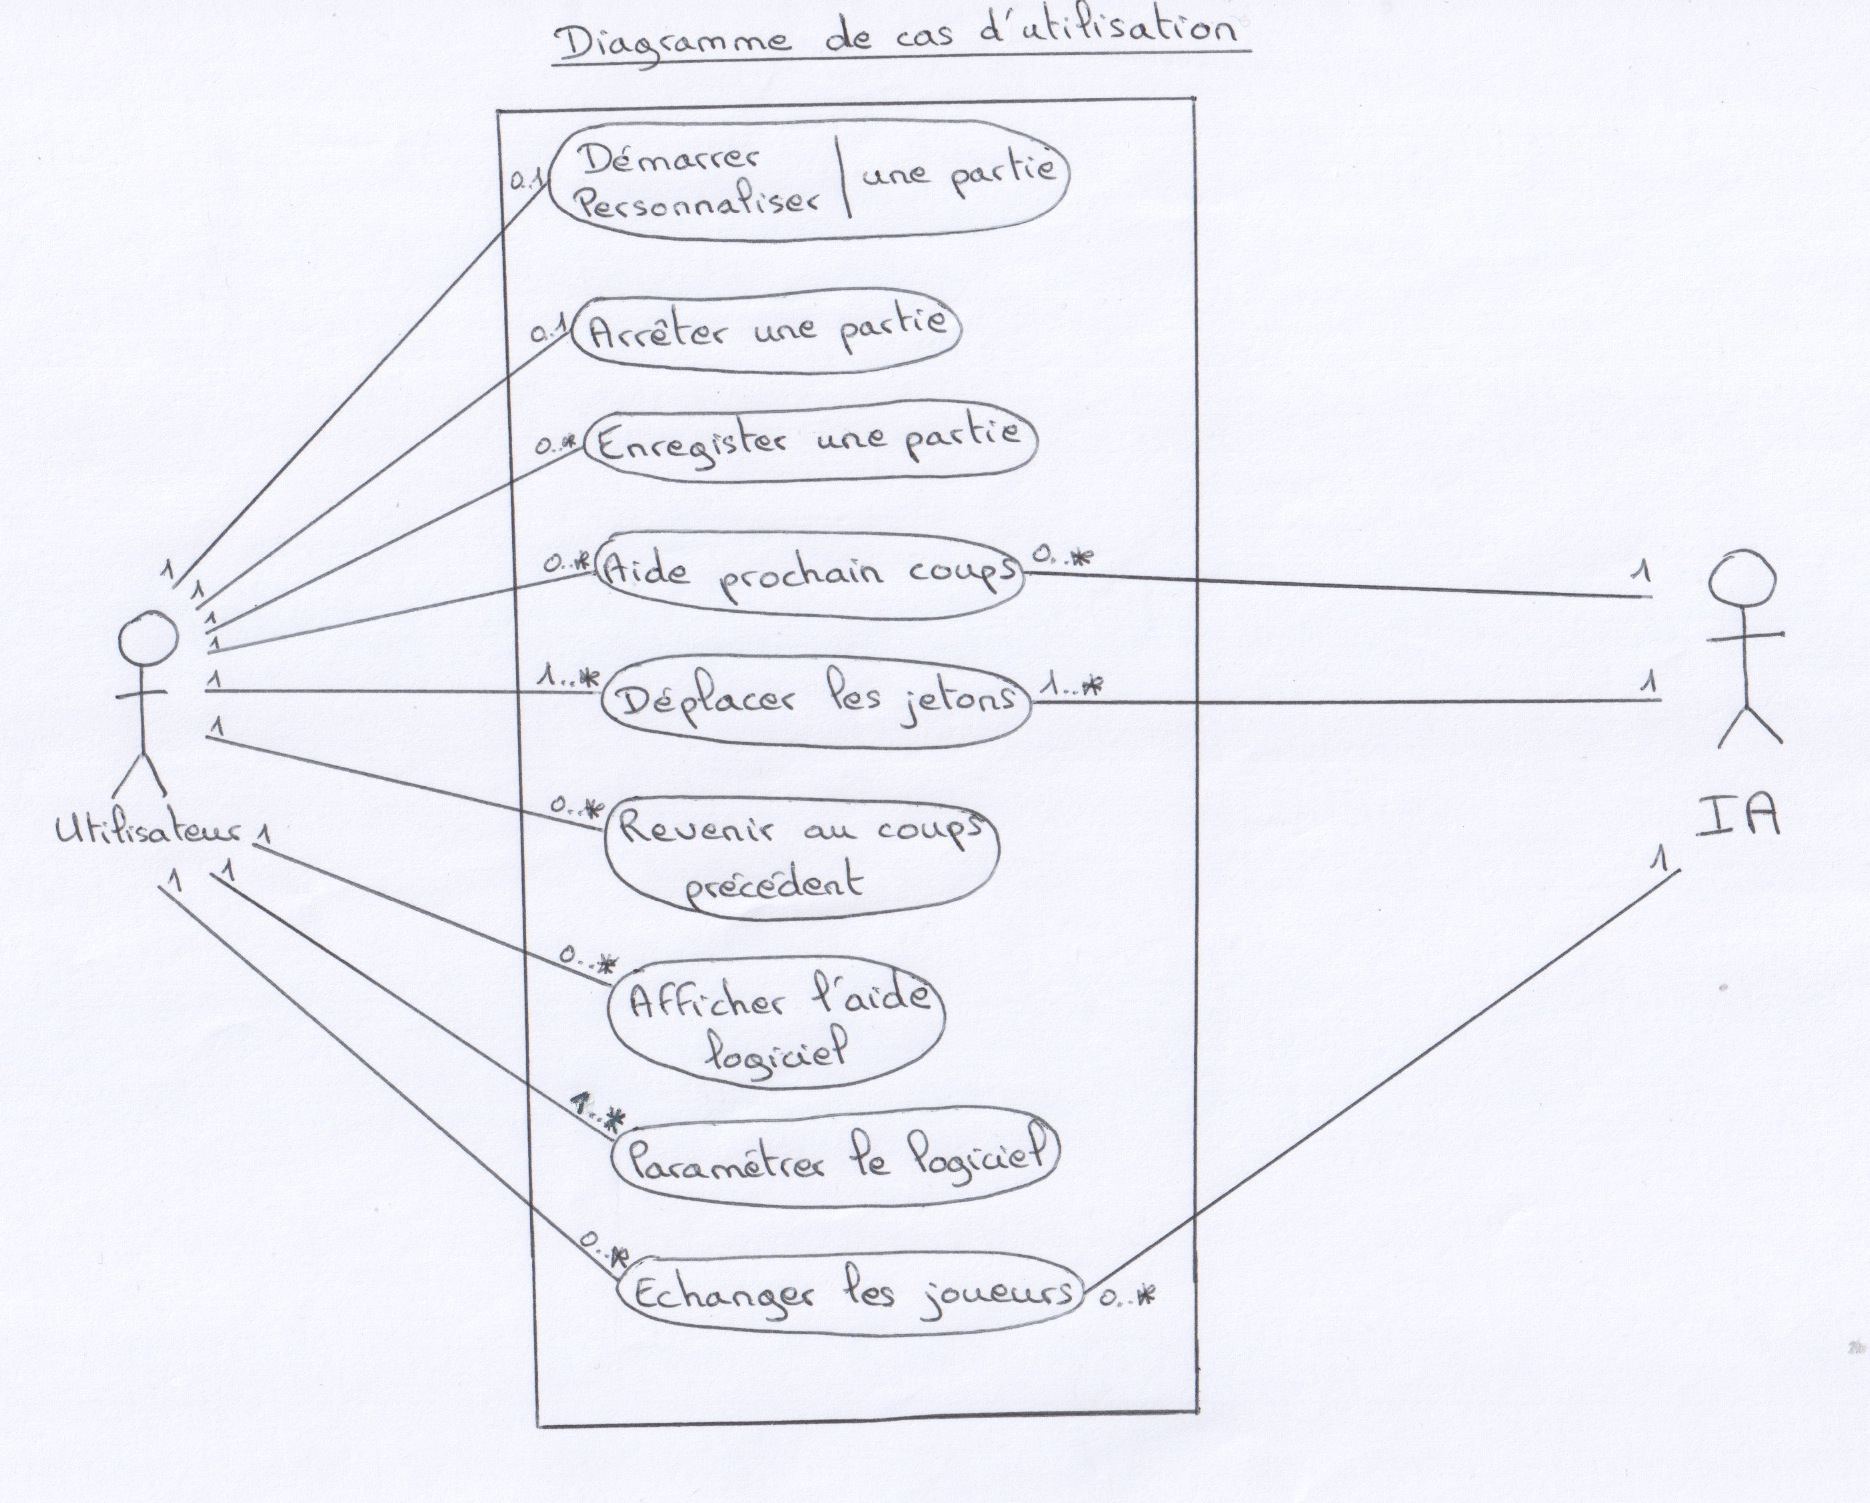
\includegraphics[scale=0.7]{cas-utilisation.jpeg}
\caption{Diagramme UML des cas d'utilisation du logiciel}
\label{cas}
\end{figure}


\section{Diagramme de machine à états}
\label{C}
\begin{figure}[H]
  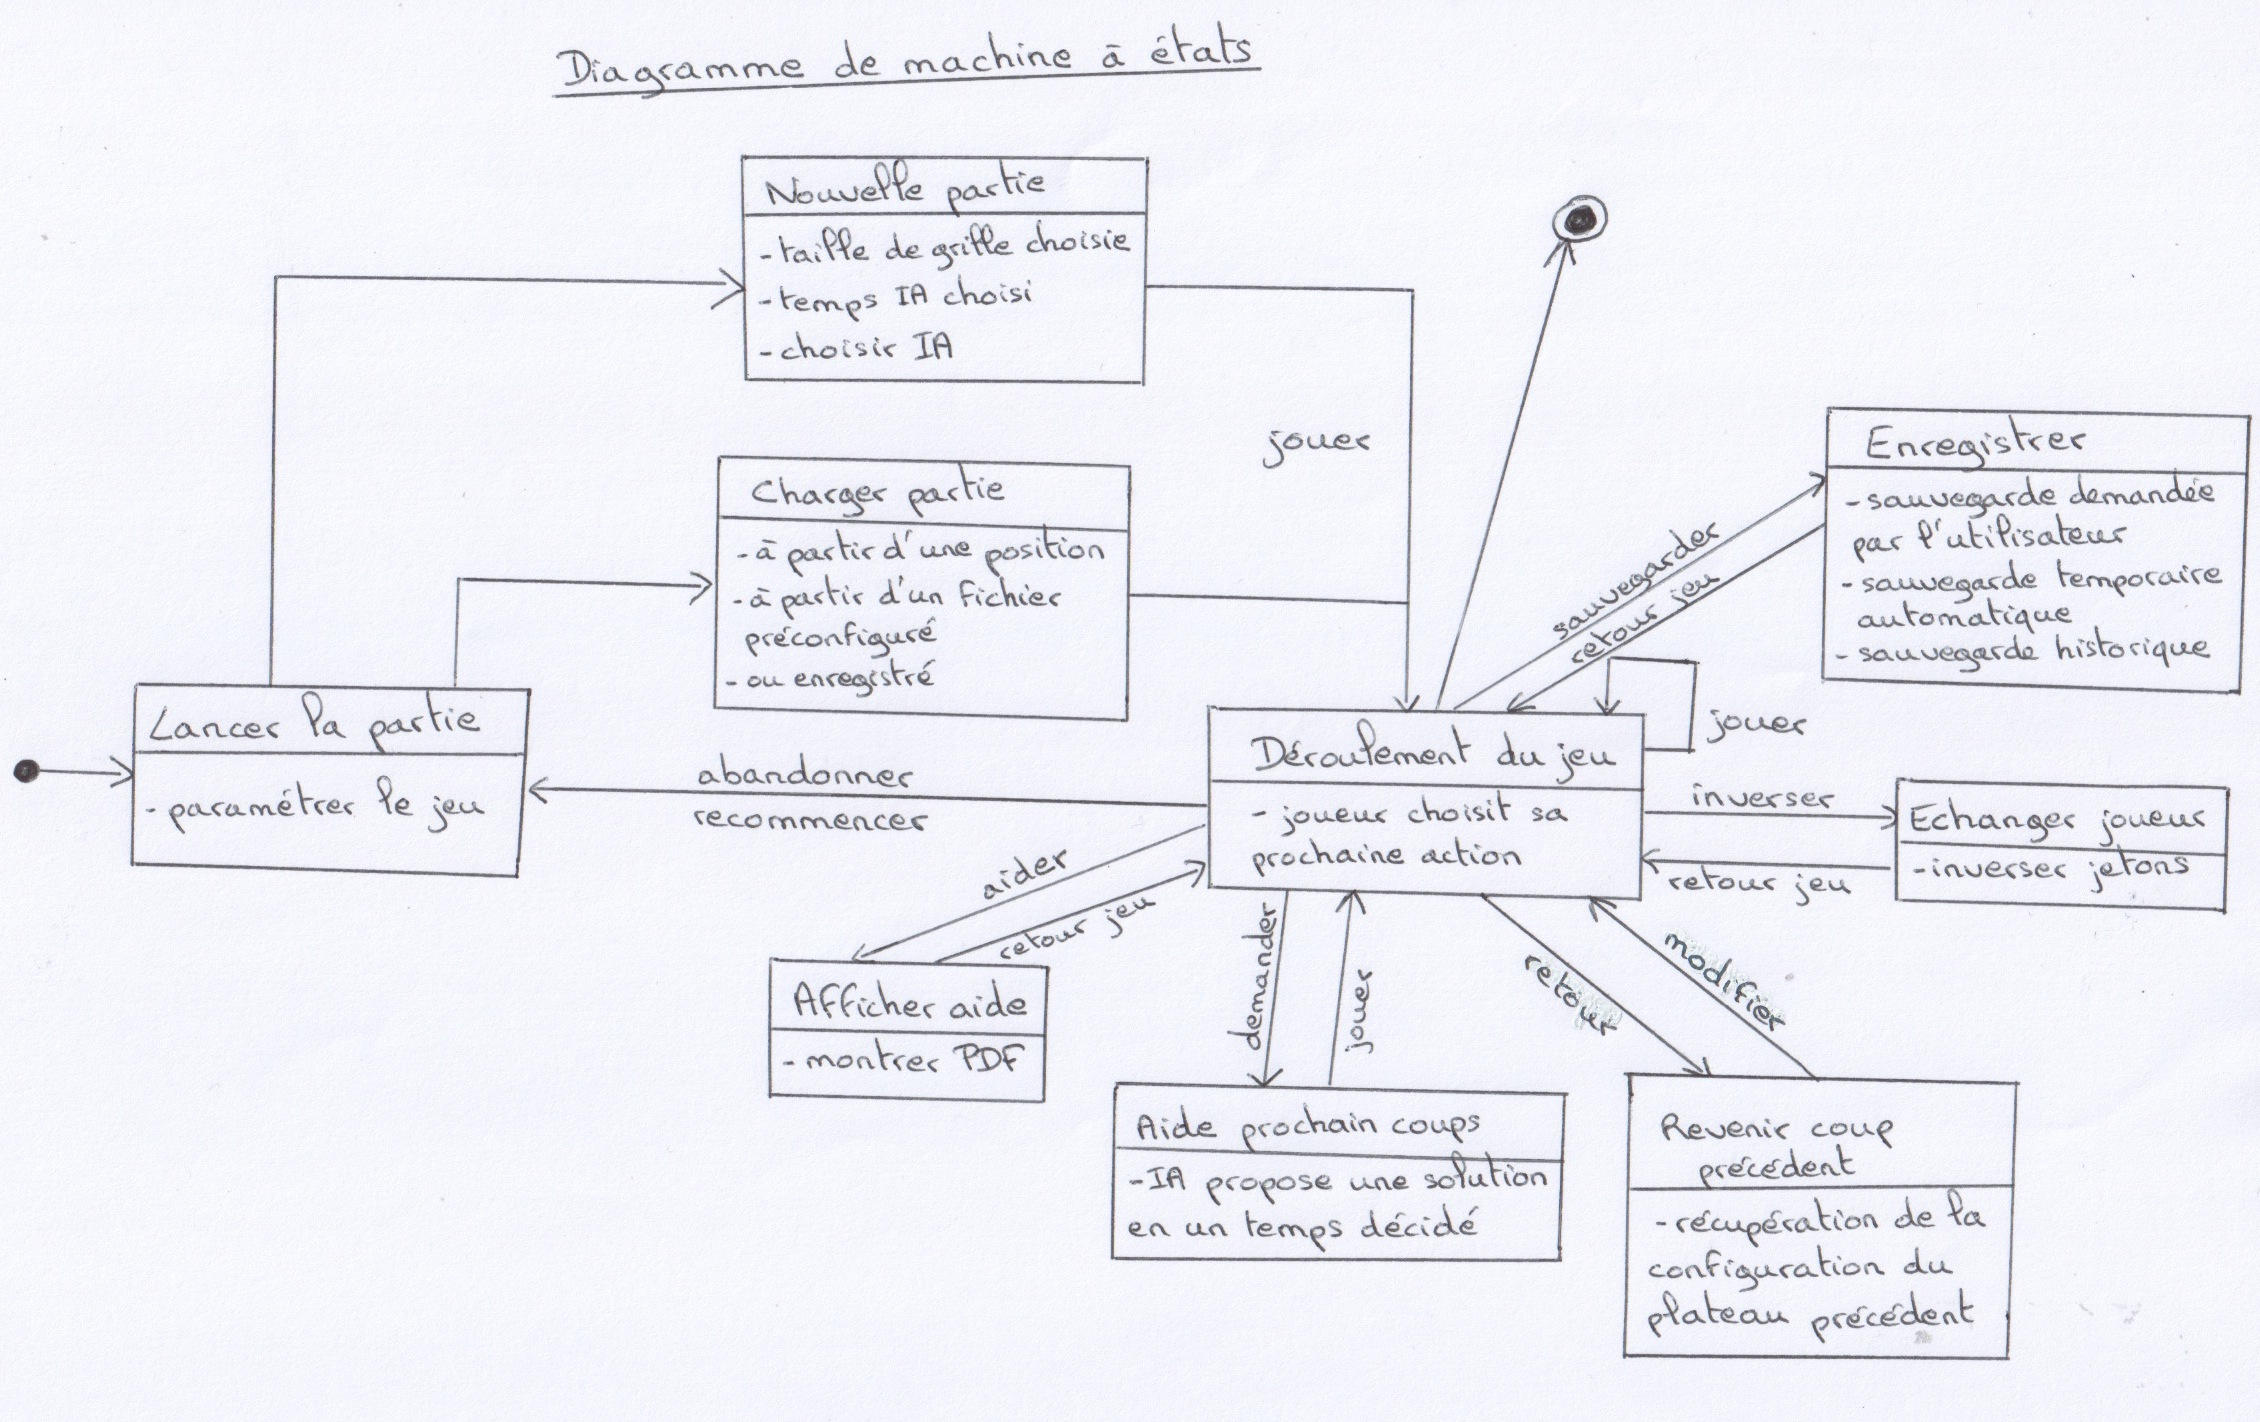
\includegraphics[scale=0.6]{machine-etat.jpeg}
\caption{Diagramme UML de machine à états}
\label{etat}
\end{figure}


\section{Prototypes papier de l'interface}
\label{D}

\begin{figure}[H]
\includegraphics[scale=0.1]{plateau.jpg}
\caption{Plateau de jeu comprenant la grille, les menus et les
  boutons}
\label{plateau}
\end{figure}

\begin{figure}[H]
\includegraphics[scale=0.1]{position.jpg}
\caption{Prototype de la fonctionnalité de retour en arrière pour des coups}
\label{retour}
\end{figure}

\begin{figure}[H]
\includegraphics[scale=0.1]{boutons.jpg}
\caption{Prototype des boutons et des menus pour l'interface}
\label{boutons}
\end{figure}

\end{document}




\chapter{Architecture et description du logiciel}

\documentclass[a4paper,12pt]{article} 
\usepackage[utf8x]{inputenc} 
\usepackage[french]{babel} 
\usepackage[colorlinks=true,urlcolor=blue,linkcolor=blue]{hyperref}
\usepackage[T1]{fontenc}
\usepackage[cm]{fullpage}
\usepackage{url}

\usepackage{graphicx}
\usepackage{float}
\usepackage[toc,page]{appendix}


\renewcommand{\appendixtocname}{Annexes}
\renewcommand{\appendixpagename}{Annexes} 
\addto\captionsfrench{\def\tablename{{Tableau}}}
\begin{document}

\title{Analyse des besoins et tests pour le projet\\
  \textit{Réalisation d'un jeu d'Othello}}

\author{Morgane Badré\\
  Benjamin Letourneau,\\
  Vincent Wilmet,\\
  Nicolas Yvon\\}
\date{}

\maketitle

Ce document présente une version préliminaire de l'architecture de notre projet.

\section{Architecture du projet}
Le projet à développer est conséquent, certains modules à réaliser sont plus compliqués que d’autres donc nous avons pensé segmenter en différentes briques. Le principe de la segmentation (voir figure \ref{glob}) en module est qu’ils sont tous indépendants et peuvent être testés indépendamment. Les blocs IA et logiciel sont les plus importants alors que la gestion de fichiers, l’interface et l'éditeur de plateau sont les moins importants. Le second intérêt de cette architecture est que chaque module peut être remplacé par un autre plus ou moins équivalent sans compromettre l’intégrité et le bon fonctionnement du logiciel. Par exemple, pour le bloc de l’IA, si une personne de la communauté souhaite l’améliorer, il peut tout simplement coder le module IA et l’intégrer au logiciel pour le tester. 

Développant en JAVA, les différents modules sont liés par le biais d’interfaces. Ainsi, chaque module présentera une interface définie et dûment commentée qui représentera le comportement du module.


\begin{figure}[H]
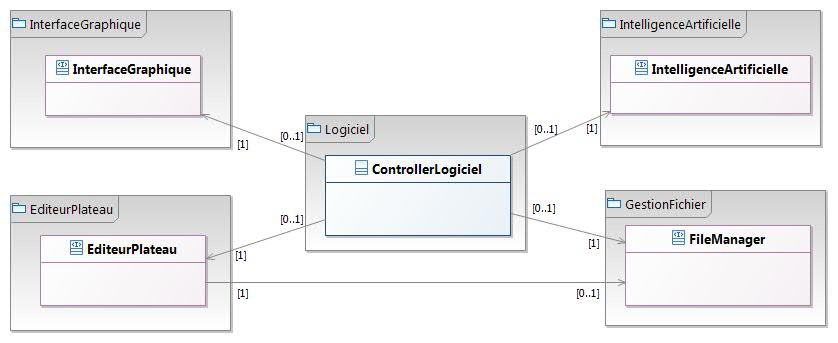
\includegraphics[scale=0.65]{ArchiProjet.jpg}
\caption{Diagramme de classe du projet global}
\label{glob}
\end{figure}

\subsection{Module Logiciel}

Il reprend trois design pattern : State, Factory, MVC.
\begin{itemize}
  \item State sera utilisé pour coder les différents types de pion sur le plateau
  \item Factory sera utilisé pour la génération d’objets
  \item Et l’architecture complète du logiciel sera en MVC pour la maintenabilité et la facilité de lecture/modification du code.
\end{itemize}



\subsection{Module d'Intelligences Artifcielles}

Ce module (voir figure \ref{ia}), le plus compliqué et plus important à réaliser dans notre projet, reprend le design pattern strategy. En effet, on représentera les différents types d’IA en strategie : naïve, force brute, évolutive, ...

\begin{figure}[H]
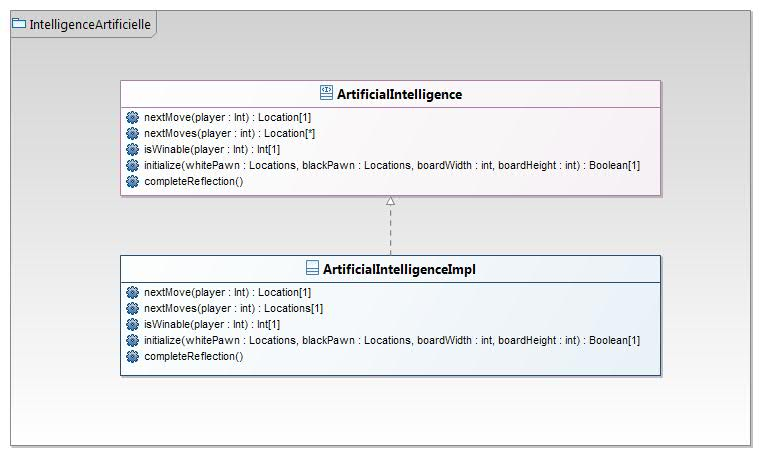
\includegraphics[scale=0.65]{IntelligenceArtificielle.jpg}
\caption{Diagramme UML de classe du module d'intelligence artifcielle}
\label{ia}
\end{figure}

\subsection{Module de Gestion de Fichier}

La gestion de fichiers (voir figure \ref{gest}) ne contient pas de design pattern spécifique.

\begin{figure}[H]
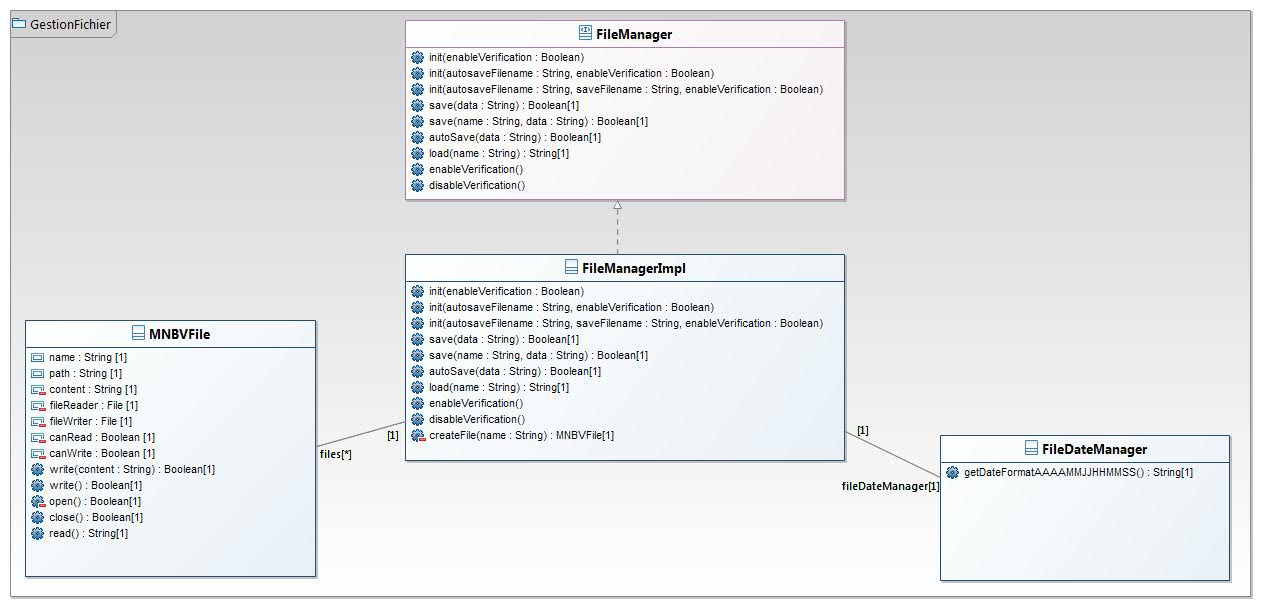
\includegraphics[scale=0.42]{GestionFichiers.jpg}
\caption{Diagramme UML de classe du module de gestion de fichier}
\label{gest}
\end{figure}

\subsection{Module d'Interface Homme-Machine (IHM)}

L’IHM ne contient pas de design pattern spécifique.


\subsection{Module d'Editeur de Plateau}

Ce module (voir figure \ref{edit}) n'utlisera pas de design pattern car si cette fonctionnalité est implémentée, elle ne sera pas forcément graphique mais plus probablement utlisable par la console donc l'architecture sera simple. 


\begin{figure}[H]
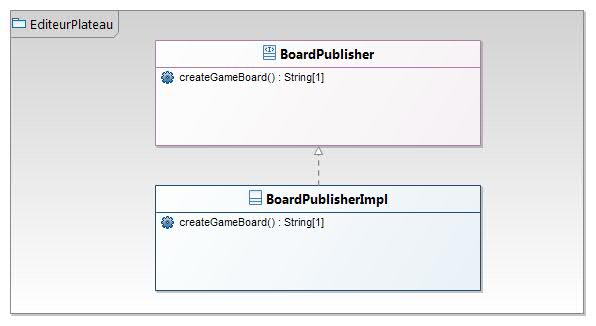
\includegraphics[scale=0.75]{EditeurPlateau.jpg}
\caption{Diagramme de classe du module éditeur de plateau}
\label{edit}
\end{figure}







\end{document}




\section{Design patterns utilisés}

Les design patterns (patron de conception, en français) ont été créés afin de remédier à certains problèmes de conception récurrents. Chacun d’eux répond à un problème précis et permet d’améliorer la maintenabilité et la réutilisation de notre code. 

Notre formation à l’approche objet en Java nous a permis de voir plusieurs de ces patterns. Nous les avons implémentés dans nos différents modules dès que l’architecture si prêtait.

\subsection{State}

Le principe de ce pattern est de pouvoir changer le comportement d’un objet sans modifier son instance, ainsi que de facilité l’ajout de nouveaux comportements. Nous l’avons utilisé afin de gérer les pièces de l’othellier.

En effet, une pièce peut être de différentes couleurs : noire, blanche ou vide (équivalent à aucune pièce). Le principal avantage de ce pattern, pour les pièces, est de pouvoir facilement changer sa couleur ou d’ajouter une nouvelle couleur si on le souhaite.

Cependant, cette implémentation a ses désavantages. Chaque changement de couleur demande une nouvelle instanciation de comportement et donc, une partie de la mémoire. C’est pour cela que pour les calculs lourds des intelligences artificielles, ce pattern n’a pas été utilisé.

Nous avons également utilisé ce pattern sur la classe Joueur. Celle-ci contient deux comportements : Machine et Humain correspondant à un joueur humain décidant son coup et à l’IA qui décide son propre coup. Nous avons utilisé ce pattern dans le cas d’un comportement différent qui pourrait être demandé par le client pour améliorer l’expérience utilisateur du jeu ou dans une démarche scientifique de recherches. Prenons, par exemple, une fonctionnalité où à partir d’une certaine position dans la partie, un joueur Humain déciderait de laisser l’IA jouer à sa place. Ainsi, en changeant simplement le type de joueur, l’IA prendrait la main. Ceci est possible car à chaque pièce posée, le contrôleur général gère l’évènement associé (automatique pour l’IA et sur clique d’une case pour l’Humain) selon le type du joueur.

\subsection{Abstract Factory}

Le pattern Abstract Factory (Fabrique Abstraite) permet de fournir une interface unique et simple d’utilisation pour créer les objets d’une même famille sans avoir à connaître la classe à instancier. Nous avons utilisé ce pattern dans le module Othello Kernel notamment sur les objets “package Model”.

Notre fabrique abstraite (classe AbstractFactory) permet de gérer plusieurs fabriques, à savoir celles de “Piece”, de “Player”, “Board”, “GameSettings”, et de “Save/RestoreGame”. Chacune d’elle permet de gérer un type d’objet précis. Ainsi, nous avons plusieurs “factory” ; une pour chaque classe citée ci-dessus. Toutes ces “factory” sont elles mêmes interfacées par une classe abstraite “AbstractFactory” et récupérables par l’intermédiaire de la classe “FactoryProducer”.

Ce pattern présente, malgré tout, plusieurs inconvénients. Premièrement, il est compliqué à mettre en place car chaque fabrique d’objets à besoin d’une classe et d’une interface. De plus, toutes les “factory”, quel que soit leur comportement, doivent implémenter les mêmes méthodes car elles interfacent toute la même classe abstraite. Ainsi, nous avons sécurisé chaque comportement inapproprié pour chaque “factory” par un système d’exceptions. Finalement, chaque fabrique étant liée à la même classe abstraite, la modification d’une signature de méthode se répercute sur toutes les “factory” entrainant des modifications profondes. 

Malgré cette mise en place relativement lourde, ce pattern est pratique notamment lors de mises en place d’évolutions du logiciel, de maintenance, pour sa facilité d’ajout de constructeurs et également pour segmenter le code.

\subsection{Observer}

Le pattern Observer permet de réduire les dépendances d’objet mais également de gérer des évènements déclenchés par un objet observé et suivi par un observateur. Il est indispensable pour nous, pour la gestion de l’affichage de l’othellier. 

En effet, à chaque modification de l’othellier celle-ci doit être représentée visuellement sur la fenêtre utilisateur. Ainsi, la zone de dessin (GameCanvas), représentant l’othellier sous forme de grille, espionne le modèle contenant l’othellier et affiche la grille à chaque modification : ajout d’une pièce, calcul des pièces jouables …

\subsection{Model-View-Controller}

Modèle-Vue-Contrôleur permet de séparer dans une application intéractive les différents composants. La vue permet l’intéraction avec les utilisateurs, le modèle contient les données et le contrôleur gère les évènements utilisateurs et la modification de données.

Ce pattern utilise également le patron “Observer”. En effet, les données du modèle sont liées à la vue afin que celles-ci reflètent les changements à chaque modification.

Ce patron a été utilisé pour gérer le jeu Othello. Nous avons séparé le jeu en trois packages correspondant aux modules MVC. Les accès entre les modules Vue-Contrôleur et Vue-Modèle sont entièrement interfacés pour bien segmenter le code. 

\subsection{Singleton}

Ce design pattern permet de restreindre l’instanciation d’une classe à un unique objet. Nous l’avons utilisé à plusieurs reprises dans le projet. 

Toutes les diverses classes implémentant les “factory” suivent ce pattern afin de limiter l’espace mémoire utilisé. De plus, il n’est pas nécessaire d’avoir plusieurs objets pour une même factory dans notre projet.

Ce pattern a également été utilisé pour la classe Application afin d’empécher la multi-instanciation. En effet, le but de cette classe est d’être unique/”constante” pour tout le logiciel afin que chaque classe ayant besoin de ces informations puissent y accéder sans dupliquer de données.

Les contrôleurs du logiciel se doivent d’être uniques pour ne pas avoir de répétition d’action pour un évènement donné. Du coup, nous les avons implémentés en tant que Singleton par mesure de sécurité.

Lors des tests de performance, nous nous sommes rendus compte que nous avions un important problème d’optimisation mémoire. En effet, à chaque changement d’état d’une pièce, nous faisons une nouvelle instanciation correspondant à la nouvelle couleur : blanche ou noire. Afin d’améliorer nos performances mémoires, la couleur noire/blanche étant la même pour toutes les pièces, nous avons changé les classes codant les couleurs ”Blanche” et “Noire” pour qu’elles suivent le pattern Singleton. Ainsi, avec une unique intanciation des couleurs nous utilisons beaucoup moins de mémoire.

\subsection{Strategy}

Ce patron de conception permet de modifier dynamiquement les algorithmes utilisés. Le but étant de changer de comportement facilement selon l’environnement. Le principe repose sur l’encapsulation de ces algorithmes pour les rendre interchangeables selon les besoins.

Celui-ci a été utilisé pour la gestion des difficultés de l’IA. En effet, selon la difficulté, l’IA n’utilise pas les mêmes algorithmes : elle change de stratégie selon la difficulté choisie.

Par exemple, en mode facile le calcul de position est basé sur un algorithme aléatoire alors qu’en mode difficile celui-ci est basé sur un algorithme brute force.

\section{Heuristiques et Algorithmes de recherches de solution}

Il existe beaucoup de stratégies (voir \cite{strategy}, \cite{13}) permettant de jouer à Othello. Chacune a ses propres spécificités comme par exemple, maximiser le score des pions, empêcher le joueur d'encercler l'autre joueur, donner le moins de coups possibles à l'adversaire,... Nous avons implémenté la stratégie positionnelle, la mobilité, et la maximisation.

\subsection{Stratégie positionnelle}

Le principe de la stratégie positionnelle (voir \cite{strategy}) est de donner des scores aux cases vides du plateau en fonction de leur stabilité, semi-stabilité et de leur instabilité. Une case est dite stable ou définitive si elle ne peut être reprise par l’adversaire lorsqu’on l’aura jouée. Une case est dite instable lorsqu’on est sûr qu’elle pourra être reprise par le joueur adverse. Et enfin, une case est dite semi-stable lorsque la probabilité que le joueur adverse puisse la reprendre est moyenne.
Ainsi, on peut déjà classer quelques cases comme par exemple les coins. Les coins sont stables puisque une fois pris, ils ne peuvent être repris par l’adversaire. La case en diagonale directe de chaque coin est appelée la case X. Les cases X sont instables. De même que les cases C qui sont les 2 cases adjacentes au coin sur les bords du plateau.

\begin{figure}[H]
\centering
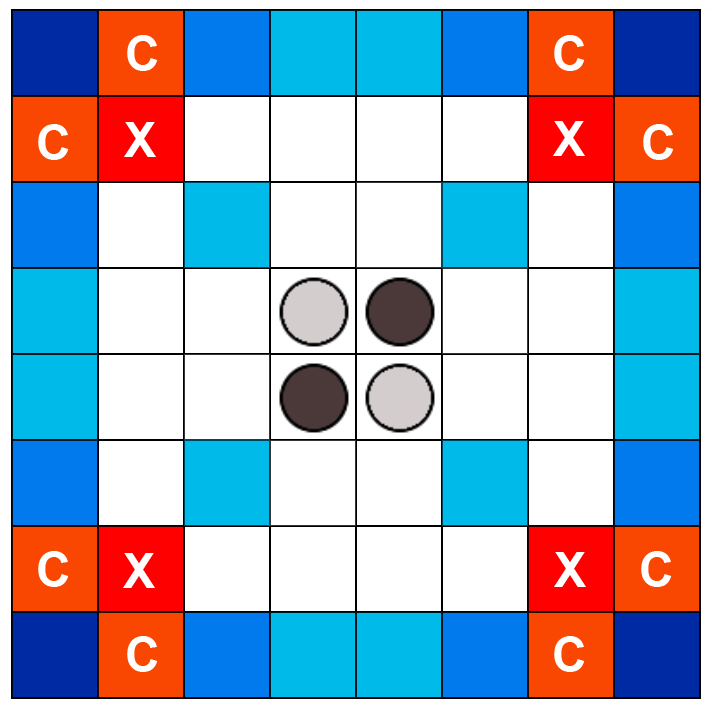
\includegraphics[scale=0.2]{Images/positionnement.png}
\caption{Grille classant les cases.}
\label{pos}
\end{figure}

Sur le schéma \ref{pos}, plus la case vire vers le rouge, plus il faut éviter de la jouer. Plus la case est bleu, plus il est intéressant de la jouer.
Ainsi, on peut créer une matrice évaluant tous les types de cases.

\begin{figure}[H]
\centering
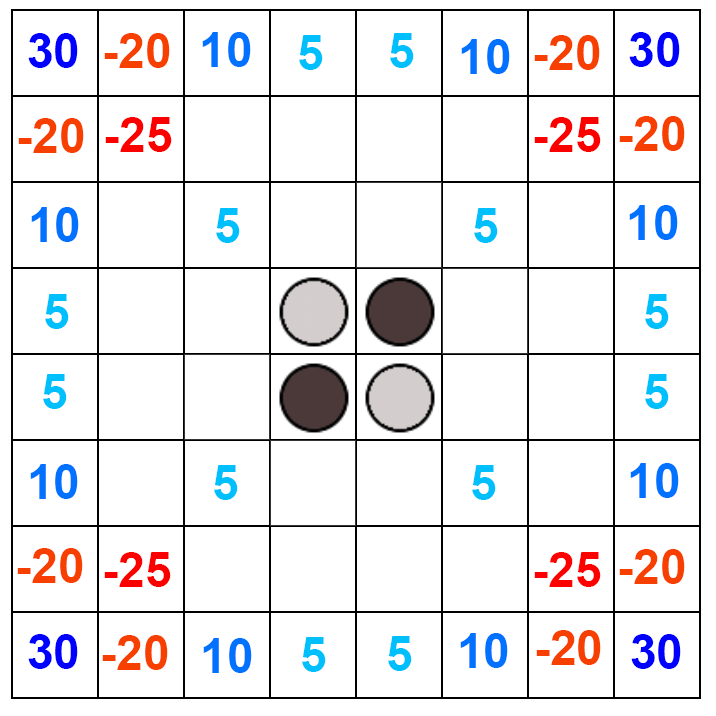
\includegraphics[scale=0.2]{Images/positionnement2.png}
\caption{Grille évaluant une partie de toutes les cases de l'othellier.}
\label{pos2}
\end{figure}

Cette matrice (figure \ref{pos2}) est alors adaptée à la taille de la grille de jeu.

Lorsque certaines configurations permettent de capturer sans crainte une position instable, celle-ci se transforme en position stable après recalcule de la matrice.


\subsection{Mobilité}

Le principe de la mobilité (voir \cite{13}) est de faire en sorte que l’adversaire ait le moins de coups possibles. Si l’adversaire a beaucoup de coups possibles, il aura certainement une plus grande probabilité de jouer un bon coup. Si l’adversaire a peu de coups possibles, il n’aura pas vraiment le choix et peut se retrouver avec des coups qui le forceront à donner facilement des pions à son adversaire. Cette stratégie est très efficace en début et en milieu de partie car elle permet de contrer toutes stratégies d’encerclement. De plus, le nombre de pièces appartenant à chaque joueur n’est pas une indication fiable pour vaincre en début et en milieu de partie donc, il faut se concentrer sur le fait de diminuer le nombre de coup du joueur afin d’avoir un net avantage lorsqu’on passera à une stratégie de maximisation...


\subsection{Maximisation}

La maximisation est une stratégie dont le principe est de capturer le plus de pièces possibles afin d’avoir le meilleur score. Cette stratégie est la meilleure en apparence puisqu’elle représente l'objectif final du jeu, à savoir obtenir plus de pions que son adversaire. Ceci est vrai si on calcule l’arbre entier de partie représentant toutes les parties possibles du jeu à partir de tous les coups jouables de toutes les positions de plateau. C'est ce qui est plus communément appelé un algorithme "brute force" ou force brute. Cet arbre donne alors le déroulement d'une partie coup après coup jusqu'à atteindre la fin, les feuilles de l'arbre.


\subsubsection{MiniMax : parcours exhaustif de l'arbre des parties}

L'algorithme MiniMax (voir \cite{1}) permet de parcourir exhaustivement l'arbre de partie du jeu et de décrire des chemins gagnants pour les deux joueurs. 
Pour cela, il calcule tous les enchaînements de coup possible à partir de la position de base du jeu. Une fois arrivée à une racine, il prend le score du joueur Max et le remonte. S'il y a plusieurs branches au niveau d'un noeud, le noeud prendra le score maximal des branches si c'est le tour du joueur Max (joueur qui maximise le score) ou prendra le score minimal si c'est le tour du joueur Min (joueur qui minimise le score).

\begin{figure}[H]
\centering
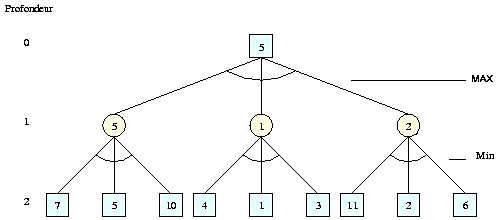
\includegraphics[scale=0.8]{Images/minimax.png}
\caption{Arbre MiniMax de profondeur 2.}
\label{minima}
\end{figure}

L'arbre de partie pouvant être tellement grand qu'il est impossible pour un ordinateur à l'heure actuelle de calculer et de sauvegarder un arbre de partie entier pour une grille d'Othello 8x8 en position initiale de début de jeu. C'est pour cela qu'il est nécessaire de fixer une profondeur à ne pas dépasser. Ainsi, il est d'usage de lancer l'algorithme en fin de partie afin d'obtenir un arbre plus petit et surtout de calculer une stratégie potentiellement gagnante pour le joueur ayant le dernier coup. Si cette stratégie est utilisée en début de partie ou en milieu, elle sera facilement battue par une stratégie positionnelle ou de mobilité puisque l'arbre ne pourra en aucun cas assurer une victoire du joueur sur le long terme.\\

L'algorithme en pseudo-code est consultable en annexe \ref{codemin}.\\

Il existe cependant plusieurs améliorations de l'algorithme MiniMax permettant d'élaguer des branches de l'arbre, l'allégeant quelque peu.


\subsubsection{L'élagage Alpha-Beta}

L'élagage Alpha-Beta (voir \cite{1}) reprend le principe de l'algorithme MiniMax en ajoutant des bornes alpha et beta afin d'éviter l'exploration de branches inutiles de l'arbre. En effet, il suffit de passer aux noeuds les valeurs actuelles de ces bornes qui changent de valeur au fur et à mesure de la recherche. Alpha représente pour un noeud MIN n, la plus grande valeur connue pour un noeud MAX ancêtre de n. Beta représente pour un noeud MAX n, la plus grande valeur connue pour un noeud MIN ancêtre de n.

\begin{figure}[H]
\centering
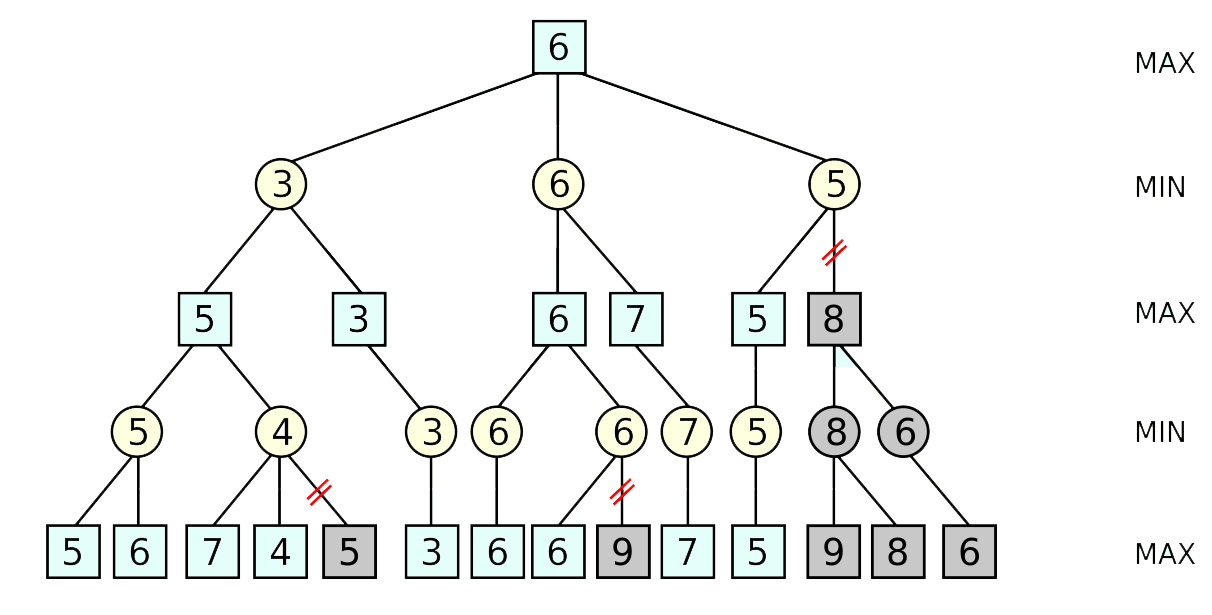
\includegraphics[scale=0.3]{Images/alphabeta.png}
\caption{Arbre Alpha-Beta de profondeur 4.}
\label{alphabet}
\end{figure}


L'algorithme utilise le début de la recherche de solution afin de borner les valeurs possibles de la racine. On élague ainsi des sous-arbres entiers de manière non risquée.\\

L'algorithme en pseudo-code est consultable en annexe \ref{codealpha}.\\

Nous avons implémenté trois autres versions un peu plus efficace pour cette algorithme:

\begin{itemize}
\item La version NegaMax est une version conventionnant l'utilisation de l'algorithme. Elle permet d'éviter la distinction entre les deux joueurs Max et Min et simplifie ainsi le code.

\item La version fail soft alpha-beta utilise un nouveau pivot dans la recherche afin de rajouter une borne current permettant d'accélerer la recherche.

\item La version NegaScout ou appelé également Principal Variation Search effectue des pré-recherches sur l'arbre en utilisant un intervalle plus petit (alpha, alpha + 1 à la place d'alpha, beta en début d'algorithme) afin d'élaguer d'avantage de branche inutile.

\end{itemize}


\chapter{Fonctionnement et tests}

A ce jour, nous avons développé l’intégralité des besoins fonctionnels. Néanmoins, nous aurions pu, si nous avions eu plus de temps, ajouter des optimisations, des améliorations, supprimer davantage de bugs.

\section{Etat du projet}

Comme décrit dans la partie 3 de ce rapport (Architecture et description du logiciel), nous avons découpé le projet en différents modules que nous allons décrire. 

\subsection{Logiciel}

Au lancement du jeu (figure \ref{cap1}), quelques réglages sont à faire avant de pouvoir jouer. Dans un premier temps, il faut indiquer la taille de la grille (le maximum est 50*50). Puis, lancer le BenchMark (explication ci-dessous) et indiquer la difficulté souhaitée. Enfin, préciser si l'on joue entre joueurs ou un joueur contre l'IA. 

\begin{figure}[H]
\centering
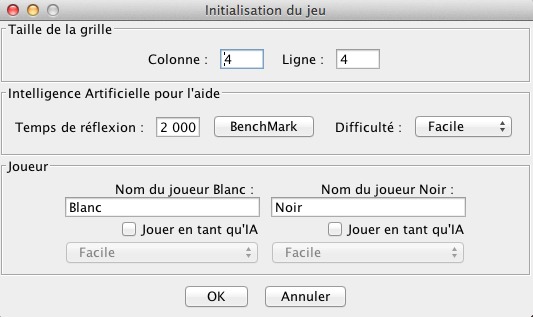
\includegraphics[scale=0.6]{Images/initialisation.png}
\caption{Initialisation du jeu}
\label{cap1}
\end{figure}

Le Benchmark (figure \ref{cap2}) permet d'évaluer les performances de la machine. En fonction du temps de réflexion obtenu, on en déduit le temps qu'il faudra à l'IA pour jouer. Celui-ci ne permet pas, actuellement, de récupérer le temps qu'il faudrait associé à l'IA mais uniquement l'indice de performance de la machine. 

\begin{figure}[H]
\centering
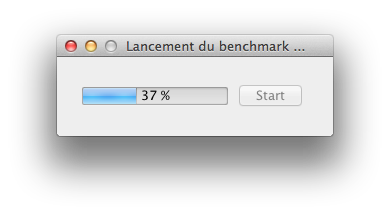
\includegraphics[scale=1]{Images/benchmark.png}
\caption{Lancement du BenchMark}
\label{cap2}
\end{figure}

Après avoir paramétré le jeu (figure \ref{cap3}), les jetons sont placés au centre du plateau et par défaut c'est le joueur blanc qui commence. 

\begin{figure}[H]
\centering
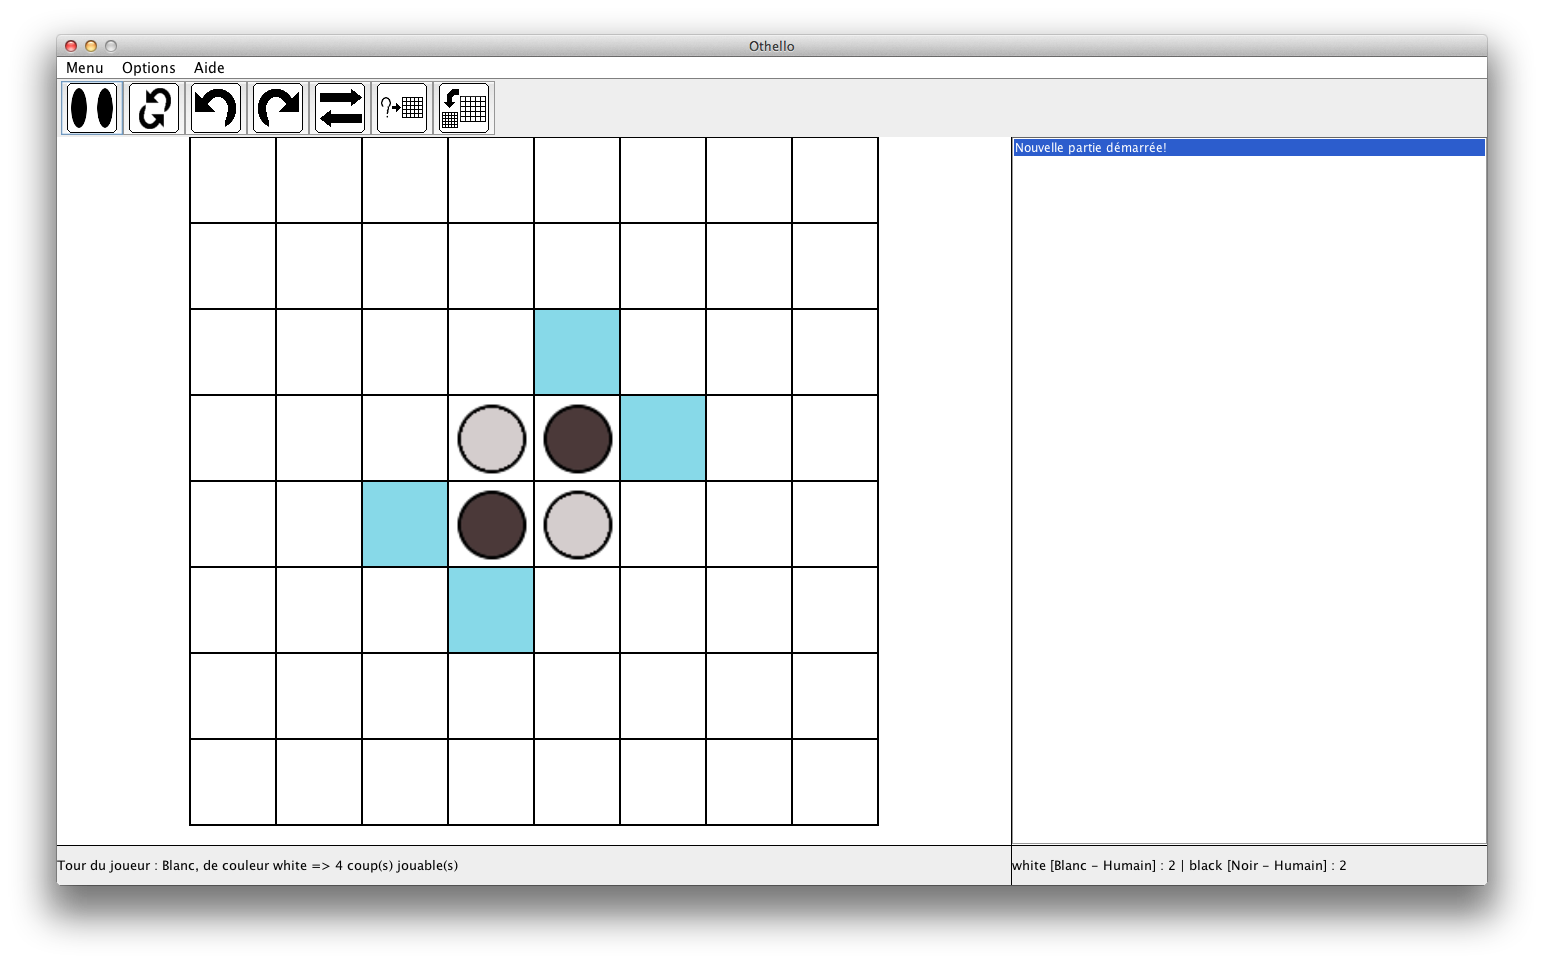
\includegraphics[scale=0.2]{Images/debut.png}
\caption{Jeu de base}
\label{cap3}
\end{figure}

Le logiciel, au cours d'une partie (figure \ref{cap4}), possède plusieurs zones afin d'informer l'utilisateur : le plateau, l'historique (liste à droite), menu général en haut à gauche ainsi qu'une aide et enfin, en bas, à gauche une barre de notification et à droite, une barre de statistiques sur la partie actuelle.

\begin{figure}[H]
\centering
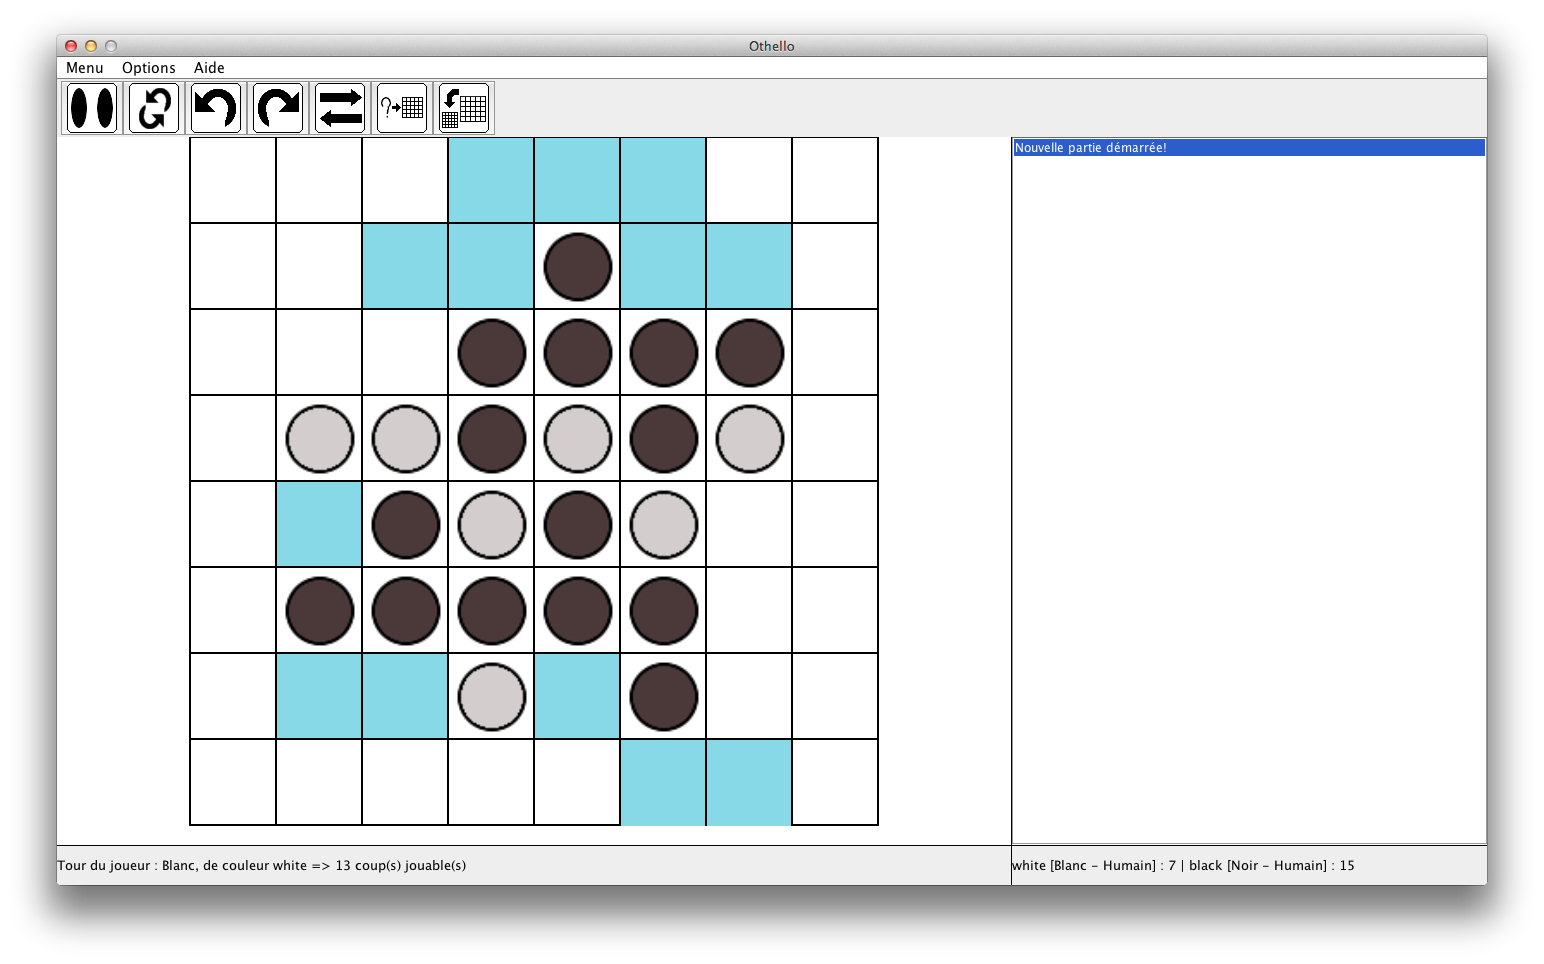
\includegraphics[scale=0.2]{Images/cours.png}
\caption{Partie en cours}
\label{cap4}
\end{figure}

Si l'utilisateur le désire, il peut choisir de revenir à n'importe quelle position jouée (figure \ref{cap5}) en cliquant sur le bouton "Revenir à une position". Ainsi, il peut recommencer une partie à une position donnée. 

\begin{figure}[H]
\centering
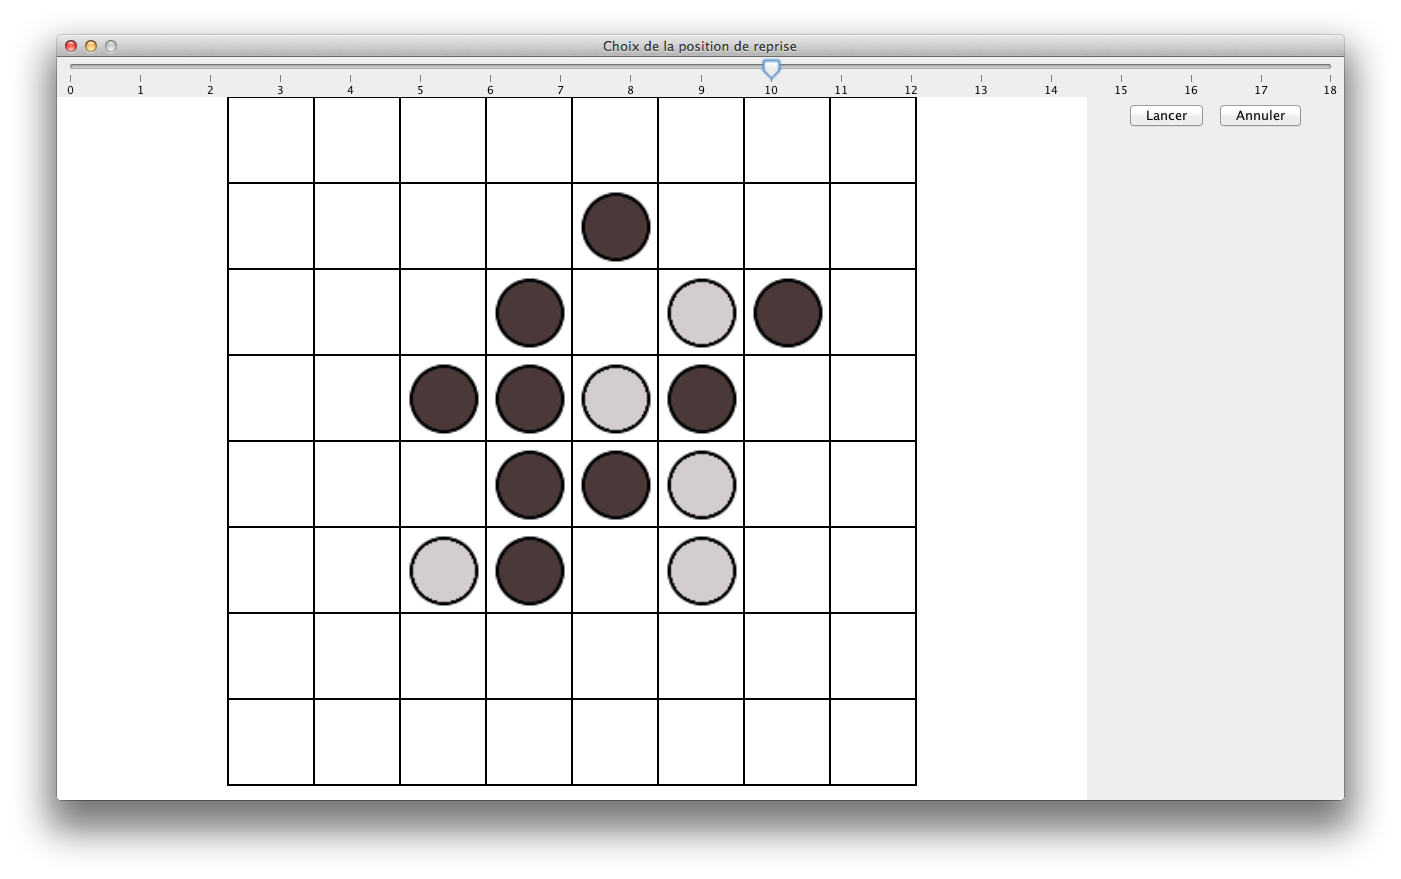
\includegraphics[scale=0.3]{Images/sliderevenir.png}
\caption{Changement de position jouée grâce au slider}
\label{cap5}
\end{figure}


\subsection{Editeur de plateau}

Afin d'accéder à ce module, vous devez aller dans le menu "Menu" puis "Configurer une partie".

Une fois le module lancé, il suffit juste de suivre les instructions à l'écran.

Vous devrez tout d'abord saisir la taille du plateau de jeu, puis préciser la grille de jeu initiale (pion par pion ou à l'aide d'un fichier préconfiguré par vos soins). Il ne vous restera plus qu'à renseigner les valeurs concernant les joueurs et l'intelligence artificielle.

Si vous voulez créer un fichier de jeu à partir d'un plateau préconfiguré, vous devrez créer un fichier evec l'extension ".grd" puis le remplir de façon à représenter la grille de jeu. Pour un emplacement vide de la grille, vous devrez mettre un tiret ("-"), pour un pion blanc, vous devrez saisir la lettre o en minuscule ("o") et pour un pion noir, vous devrez saisir l'astérisque ("*"). Pour finir avec la création de ce fichier, afin de revenir à la ligne, vous devrez utiliser la touche entrée de votre clavier ("enter").

Voici un petit exemple ce que que pourrait représenter un plateau préconfiguré sur une grille de jeu de dimension (20x15).

\begin{figure}[H]
\centering
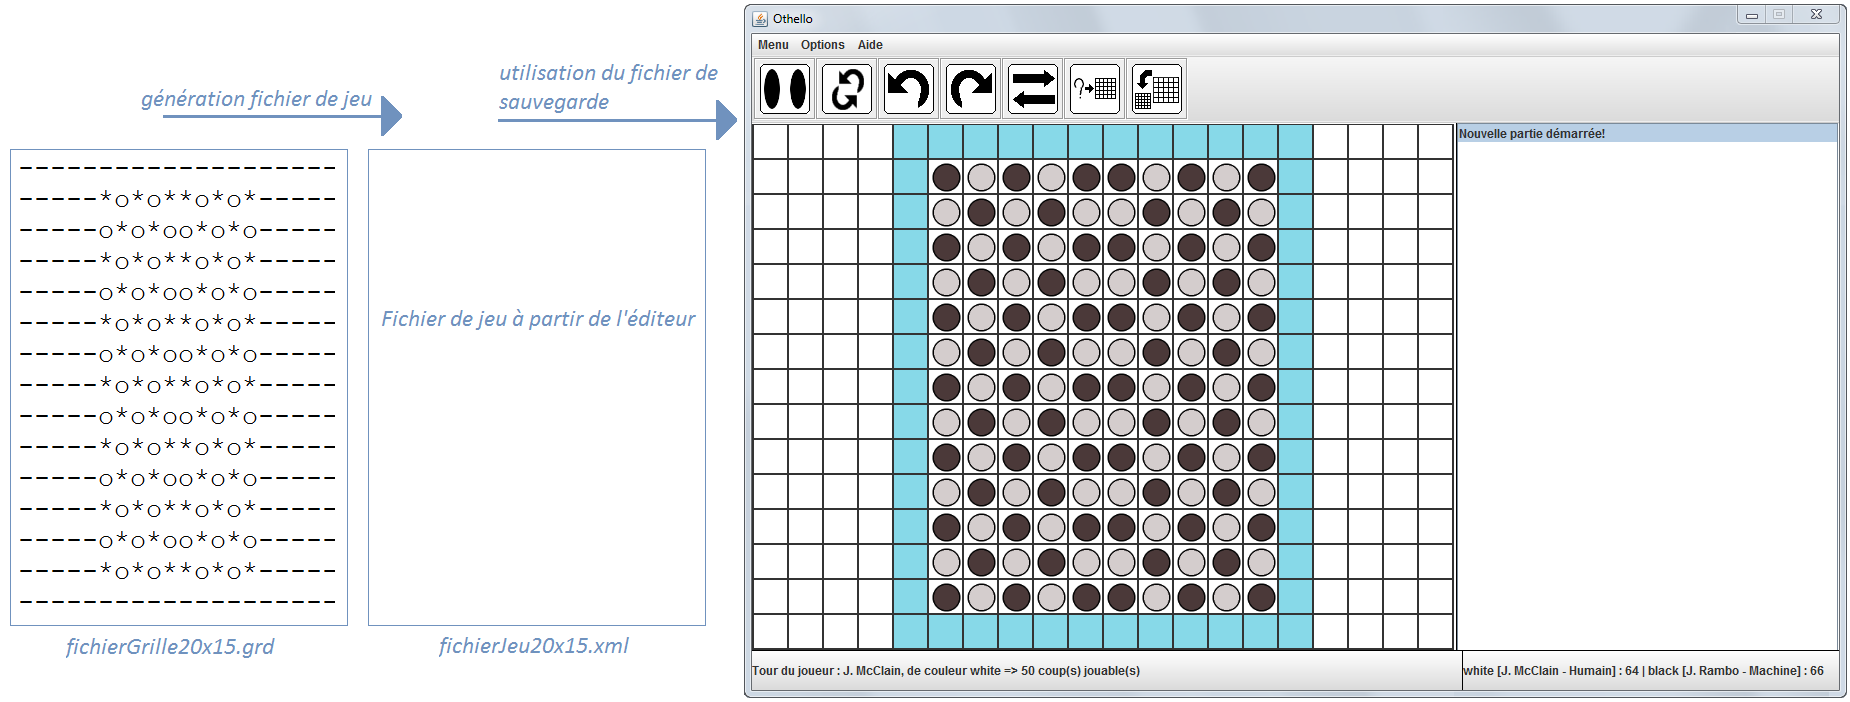
\includegraphics[scale=0.33]{Images/ExempleBP.png}
\caption{Exemple d'utilisation de l'éditeur de plateau}
\label{exbp}
\end{figure}

Attention, lors de la création du fichier de jeu, vous devez absolument passer un fichier ".grd" contenant une grille correspondant aux dimensions du plateau de jeu que vous êtes en train de créer, sinon votre grille de jeu sera standard. Elle sera aussi standard si vous saisissez un autre caractère que ceux énnoncés ci dessus.

\subsection{Aide du jeu}

Dans un premier temps, nous avions choisi de faire un fichier PDF contenant les règles et l’aide du jeu.
Finalement, nous avons décidé de développer un petit site internet en HTML5 et CSS3 qui est visible en local.  \\ 
Le site présente le projet, le jeu avec ses règles, les documents relatifs au développement, la documentation et l’équipe. 
Depuis le jeu, nous avons le bouton "Aide" qui permet d'y accéder directement.

En annexe \ref{site}, nous avons une capture ainsi que l'adresse du site hébergé sur le serveur du Cremi.

\section{Améliorations possibles sur le projet}

\subsection{Interface graphique}

Notre version étant une version Beta, il existe quelques bugs graphiques. Notamment au niveau de l'affichage du plateau. Lorsque la grille de jeu s'affiche on peut voir les cases apparaitre les unes après les autres. Cela peut géner l'utilisateur. Concernant le menu, il s'affiche parfois derrière la grille de jeu, il faut donc,  afin de pouvoir le voir dans son intégralité, réduire puis restaurer la fenêtre de jeu.

Une fonctionnalité intéressante à modifier serait l’interface d’affichage. En effet, celle-ci se rafraîchit plusieurs fois à la suite d’une pièce posée car l’ajout d’un pion entraîne plusieurs calculs qui rafraîchissent tout l’interface (exemples : action de poser un pion, calcul des pions qui se retournent, calcul des pions jouables pour l’adversaire, ...). Cette modification est très facile à implémenter grâce au pattern Observer.


\subsection{Fichier de sauvegarde}

L’une des optimisations que nous aurions pu apporter au projet concerne le module de sauvegarde (notamment l’auto-sauvegarde). En effet, lorsque l’on fait appel à la sauvegarde automatique, un nouveau fichier est créé à chaque coup joué (que l’utilisateur soit un humain ou l’intelligence artificielle). Il serait intéressant qu’à chaque fin de partie, les fichiers créés soient détruits afin de ne pas avoir occupé un espace disque trop grand au bout d’un certain nombre de parties jouées.

Comme indiqué dans le paragraphe précédent, le jeu possède un module d’édition de plateau et réalise régulièrement des sauvegardes. Le problème est que lorsque l’on veut charger une partie, le temps de chargement peut être assez long. Effectivement, il  est très rapide sur des grilles de taille standard (inférieure à 10*10), mais sur des grilles de taille 50*50 par exemple, il peut durer plusieurs secondes. La solution est donc d’exécuter le chargement d’un fichier de sauvegarde sur son propre thread afin que le reste du logiciel ne se bloque pas. 


\subsection{Module éditeur de plateau}

Nous avons développé un module de création de plateau de jeu en lignes de commande (cf. partie Etat du projet). Il serait intéressant de réaliser un éditeur de plateau de jeu graphique basé sur l’interface graphique du jeu elle-même. Du fait d’avoir réalisé une architecture du logiciel modulaire, il serait très simple de l’intégrer dans le projet.

De plus, lorsque l'on exécute le module d'édition de plateau de jeu, si l’utilisateur ne souhaite pas terminer la création de son plateau, le seul moyen pour quitter l’éditeur est de fermer complètement l’application. La solution à ce problème serait d’ajouter à l’éditeur, une fonctionnalité permettant de quitter proprement le module, et ainsi redonner la main au jeu.


\subsection{Améliorations diverses}

Lorsque nous avons testé notre logiciel sur les ordinateurs du Cremi, nous nous sommes compte que le module de gestion de fichiers ne gère pas les chemins de type /net/cremi/... mais nécessite un chemin C:\textbackslash{}...
Ainsi, il faudrait utiliser des chemins relatifs, ./chemin/..., plutôt qu'un chemin absolu. 
A cause de ces inconvénients, la sauvegarde utilisateur et le chargement ne fonctionnent pas au Cremi. 


Grâce à l’architecture choisie, l’interface peu travaillé, est facilement modifiable et de nombreuses autres fonctionnalités peuvent être facilement implémentées. Parmi ces fonctionnalités, on pourrait avoir une amélioration de l’IA qui serait évolutive, c’est-à-dire qui apprend en fonction des coups joués par l’utilisateur, s’améliorant donc au fur et à mesure de son utilisation.

Dans l’optique de rendre le jeu plus fluide et agréable à jouer nous avons créé le module BenchMark. Celui-ci attribue un chiffre à la puissance de la machine qui le lance. Nous n’avons pas eu le temps de le faire mais cela aurait été une amélioration permettant de gérer le déclenchement de certains algorithmes “gourmands” de l’IA. En effet, une machine peu puissante lancerait ces algorithmes au dernier moment pour que l’interface soit toujours réactive à l’utilisateur. Une machine puissante pourrait les lancer plus tôt dans la partie et ainsi optimiser les choix de l’IA.

Dans l’idée de rendre le jeu plus accessible nous avons codé la gestion des textes de l’interface utilisateur, pour chaque module, dans une interface. Ainsi, si l’on souhaite internationaliser le logiciel il suffit de créer une classe qui récupère le bon texte dans la langue désirée dans l’interface.


\section{Protocoles de test}

Depuis le début de nos études, c’est la première fois que nous avons à réaliser un projet aussi complet (étude bibliographique, étude des besoins, gestion d’un client, ...). Ainsi, nous n’avons pas réussi à respecter notre emploi du temps comme nous aurions dû. De ce fait, nous n’avons pas pu réaliser autant de tests que voulu. 

Pour s’assurer du bon fonctionnement de notre architecture et de notre implémentation, nous avons réalisé différents types de tests.

\subsection{Tests unitaires}

Le \textbf{test unitaire} est un procédé permettant de vérifier le bon fonctionnement d’une partie spécifique du programme. Pour se faire, nous nous sommes aidés de l’outil JUnit pour tester certaines de nos méthodes.

Parmi les tests prévus, nous en avons réalisé la plus grande partie que nous présentons ci-dessous :

\begin{itemize}
\item L’othellier choisi au chargement correspond bien à celui de la sauvegarde
\item La position choisie ne doit pas être hors des bornes
\item Lorsque l’IA suggère un coups, la position de celui-ci doit correspondre à un coup valide
\item La grille générée doit avoir la taille demandée
\item Le temps de réflexion alloué à la réflexion de l’IA doit être respecté
\item Tester visuellement que les jetons sont correctement échangés avec ceux de l’adversaire lors du changement de joueur
\item Changer de joueur fréquemment
\item Les fichiers de sauvegardes contiennent les informations correspondant à la partie sauvée.
\end{itemize}

\subsection{Tests d’intégration}

Le \textbf{test d’intégration} permet de vérifier le bon fonctionnement du regroupement de différents modules validés. 
Pour l’évolution de chaque module, à l’ajout ou la modification de fonctionnalités, entraînant la création d’un .jar, tous les tests d’intégration sont refaits afin de vérifier que les changements ne sont pas sources de bugs. 

\subsection{Tests fonctionnels}

Le \textbf{test fonctionnel} sert à vérifier qu’une fonctionnalité est correctement exécutée. Il se rapproche plus d’une représentation accessible au client, “personne lambda”, qu’à un expert en informatique.

Voici une liste des tests effectués :
\begin{itemize}
\item Vérifier que le résultat de la réflexion de l’IA est correct.
\item Le fichier de sauvegarde est bien créé et valide. De plus, le plateau affiché après chargement correspond bien au fichier en entrée.
\item La fonctionnalité de retour en arrière est désactivée lorsqu’il n’y a plus aucun coup précédant le coup actuel.
\end{itemize}

\subsection{Tests systèmes}

Les \textbf{tests systèmes} sont un ensemble de tests effectués pour évaluer la correspondance avec les exigences spécifiées. Ils appartiennent à la classe des tests de type boîte noire, et donc, ne nécessitent aucune connaissance au niveau développement.
Voici une liste des test effectués :
\begin{itemize}
\item Exécution du jeu simultanément à un autre logiciel (gourmand en ressources) pour vérifier que le comportement du logiciel reste inchangé.
\item Le temps de réflexion associé à l’IA doit correspondre à celui donné lors du choix utilisateur
\item Exécution du logiciel sur différentes machines de puissances différentes (netBook, ultraBook, PC de salon, PC de jeu)
\item Fermer l’application en plein milieu d’une partie, pendant la réflexion de l’IA.
\item Tester le logiciel sur différents systèmes d’exploitation supportant la JVM : Windows, Mac OS, Linux
\end{itemize}

\subsection{Tests non réalisés}

Voici quelques tests que nous n'avons pas eu le temps de faire :
\begin{itemize}
\item Test d’utilisation : Faire jouer des personnes inconnues au projet, des personnes ne connaissant pas les règles du jeu Othello, des enfants aux personnes âgées.
\item Test d’utilisation : Complément du test de Facilité d’utilisation. Faire jouer des scientifiques pouvant utiliser les résultats du programme à des fins professionnelles.
\end{itemize}

\phantomsection
\chapter*{Conclusion}

L’objectif de ce projet est de mettre en application les principes et techniques liés à la programmation vus durant notre formation telles que la gestion de projet, la programmation en Java et la documentation de code.

Travailler en quadrinôme sur un projet de 4 mois nous a permis de développer notre travail d’équipe mais essentiellement de comprendre l’intérêt d’un bon cahier des charges et d’une bonne répartition des tâches afin d’optimiser le travail de chaque personne.

Nous nous sommes rendus compte que la gestion du temps est très importante afin de tenir le planning établi.

L’ensemble des fonctionnalités demandées par le client a été implémenté. Nous avons un jeu fonctionnel où un humain peut affronter une IA en choisissant une difficulté. Deux IA peuvent également se rencontrer. Le joueur peut également créer son propre plateau ou revenir à une ancienne position jouée.

\addcontentsline{toc}{chapter}{Conclusion}


\bibliography{Existant/biblio} 

\appendix
\phantomsection
\appendixpage
\addappheadtotoc 

\chapter{Prototypes papier de l'interface}
\label{D}

\section{Prototype papier du plateau de jeu}

\begin{figure}[H]
\centering
\includegraphics[scale=0.1]{Besoins/plateau.jpg}
\caption{Plateau de jeu comprenant la grille, les menus et les
  boutons}
\label{plateau}
\end{figure}

\section{Prototype papier du retour en arrière pour les coups}

\begin{figure}[H]
\centering
\includegraphics[scale=0.1]{Besoins/position.jpg}
\caption{Prototype de la fonctionnalité de retour en arrière pour des coups}
\label{retour}
\end{figure}

\section{Prototype papier des boutons et menus}

\begin{figure}[H]
\centering
\includegraphics[scale=0.1]{Besoins/boutons.jpg}
\caption{Prototype des boutons et des menus pour l'interface}
\label{boutons}
\end{figure}

\chapter{Diagrammes UML}

\section{Diagramme de machine à états}
\label{C}
\begin{figure}[H]
\centering
  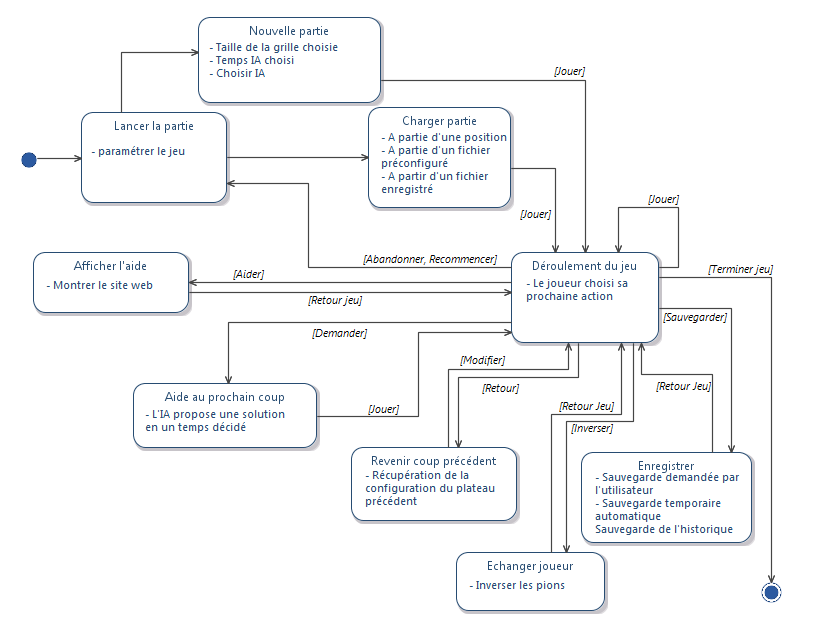
\includegraphics[scale=0.7]{Besoins/MachineEtat.png}
\caption{Diagramme UML de machine à états}
\end{figure}

\section{Diagramme de déploiement}
\label{A}
\begin{figure}[H]
\centering
  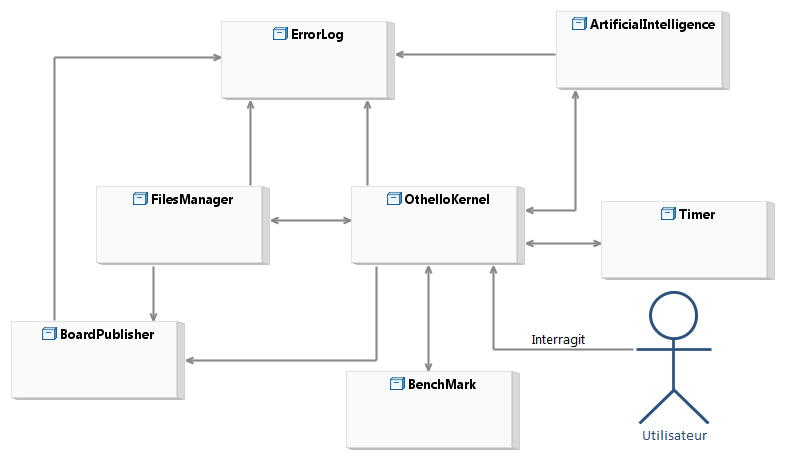
\includegraphics[scale=0.77]{Besoins/DeploymentDiagram.png}
\caption{Diagramme UML de déploiement}
\end{figure}

\section{Diagramme des cas d'utilisation}
\label{B}
\begin{figure}[H]
\centering
  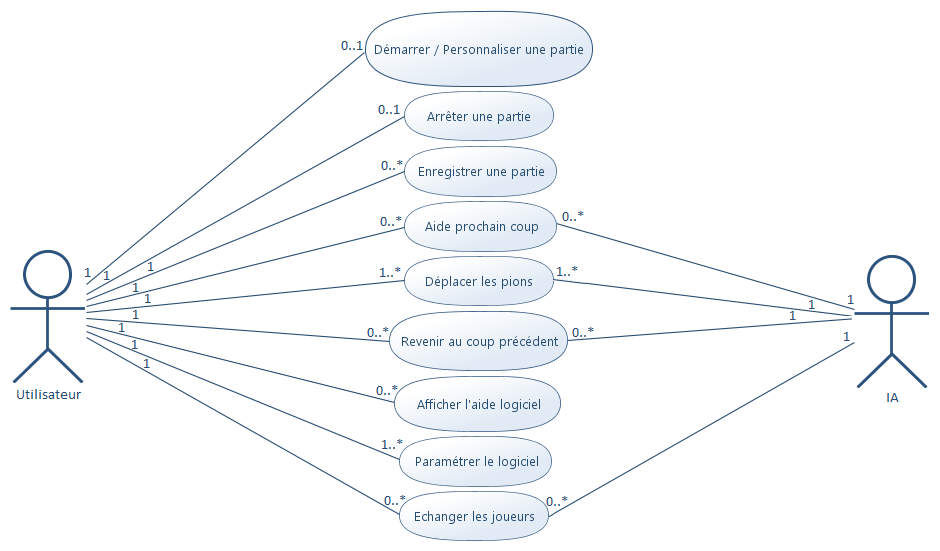
\includegraphics[scale=0.65]{Besoins/Othello_Uses_Cases.png}
\caption{Diagramme UML des cas d'utilisation du logiciel}
\end{figure}

\section{Diagramme de classes du Logiciel}
\label{OthKer}
\subsection{Model du logiciel}

\label{OthKerModel}
\begin{figure}[H]
\centering
 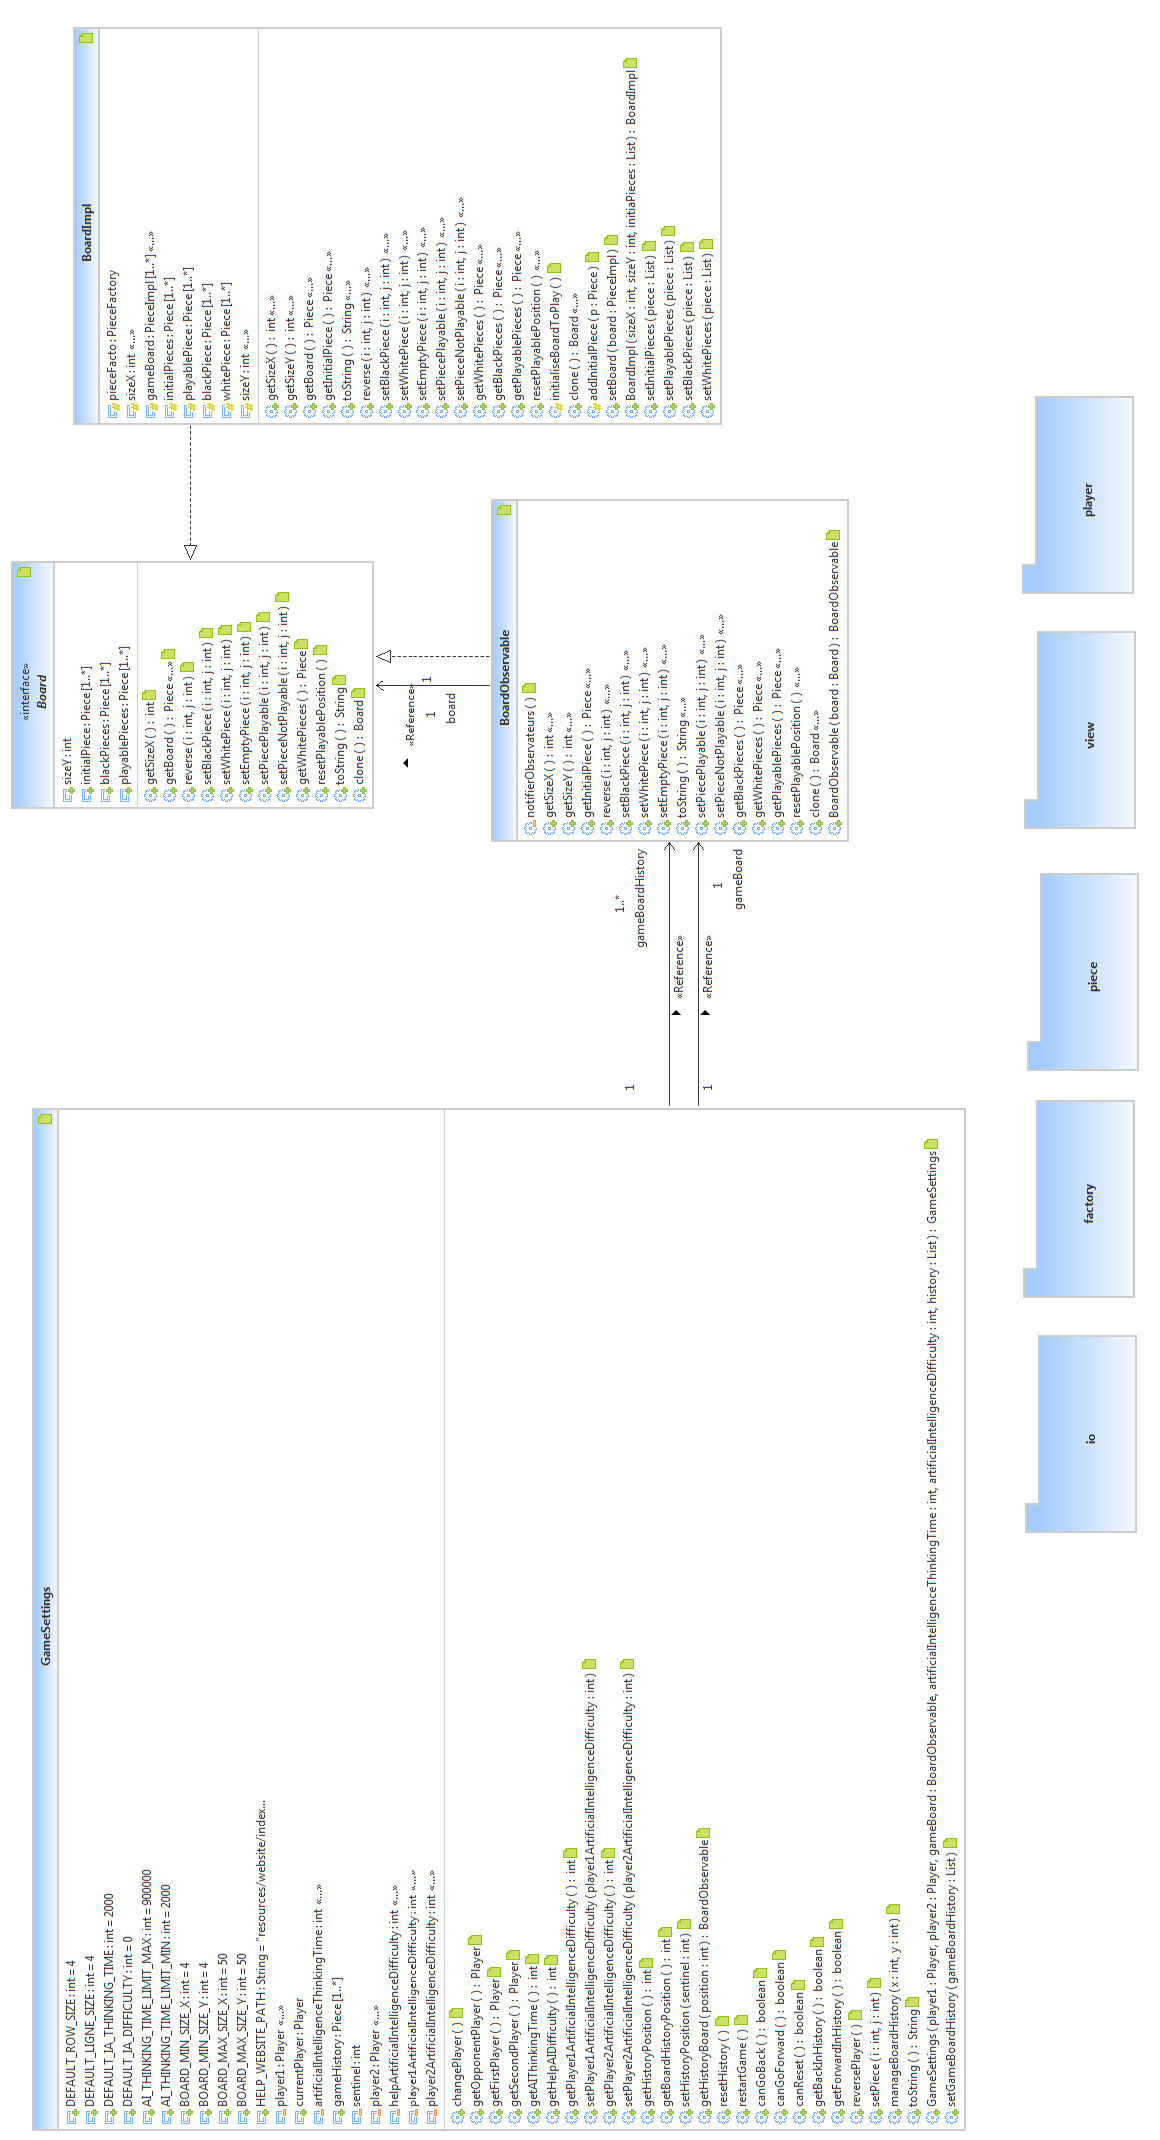
\includegraphics[scale=0.32]{Kernel/Pack_com_model.png}
\caption{Diagramme UML de classes du Package Model du Logiciel}
\end{figure}

\label{OthKerModelIO}
\begin{figure}[H]
\centering
  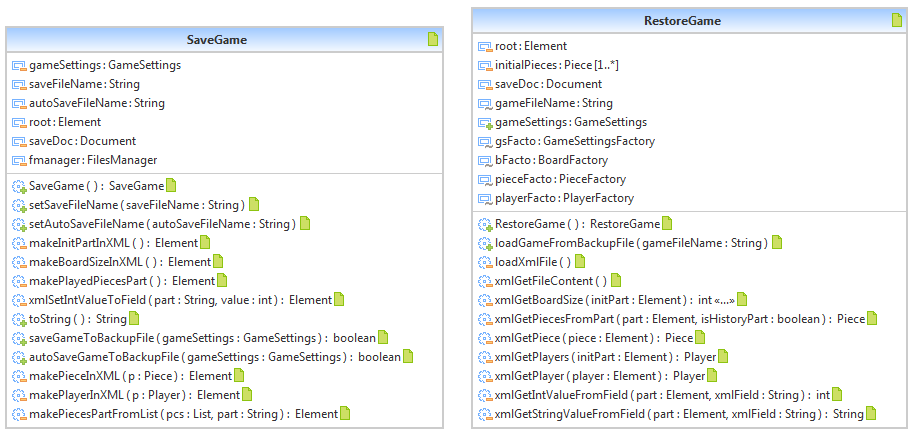
\includegraphics[scale=0.65]{Kernel/Pack_com_model_io.png}
\caption{Diagramme UML de classes du Package Model.IO du Logiciel}
\end{figure}

\label{OthKerModelPlayer}
\begin{figure}[H]
\centering
 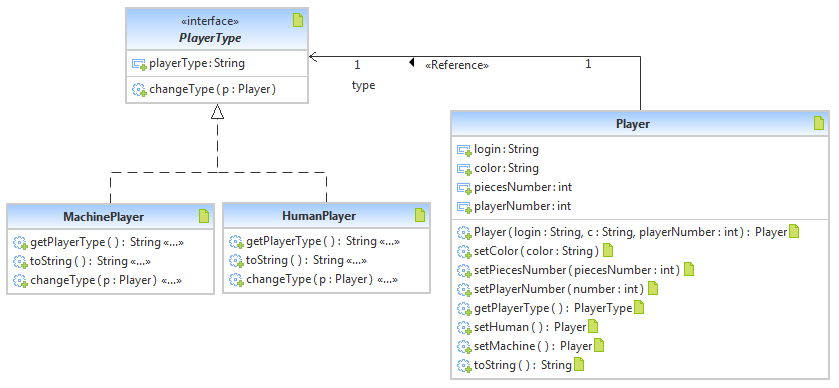
\includegraphics[scale=0.7]{Kernel/Pack_com_model_player.png}
\caption{Diagramme UML de classes du Package Model.Player du Logiciel}
\end{figure}

\label{OthKerModelPiece}
\begin{figure}[H]
\centering
 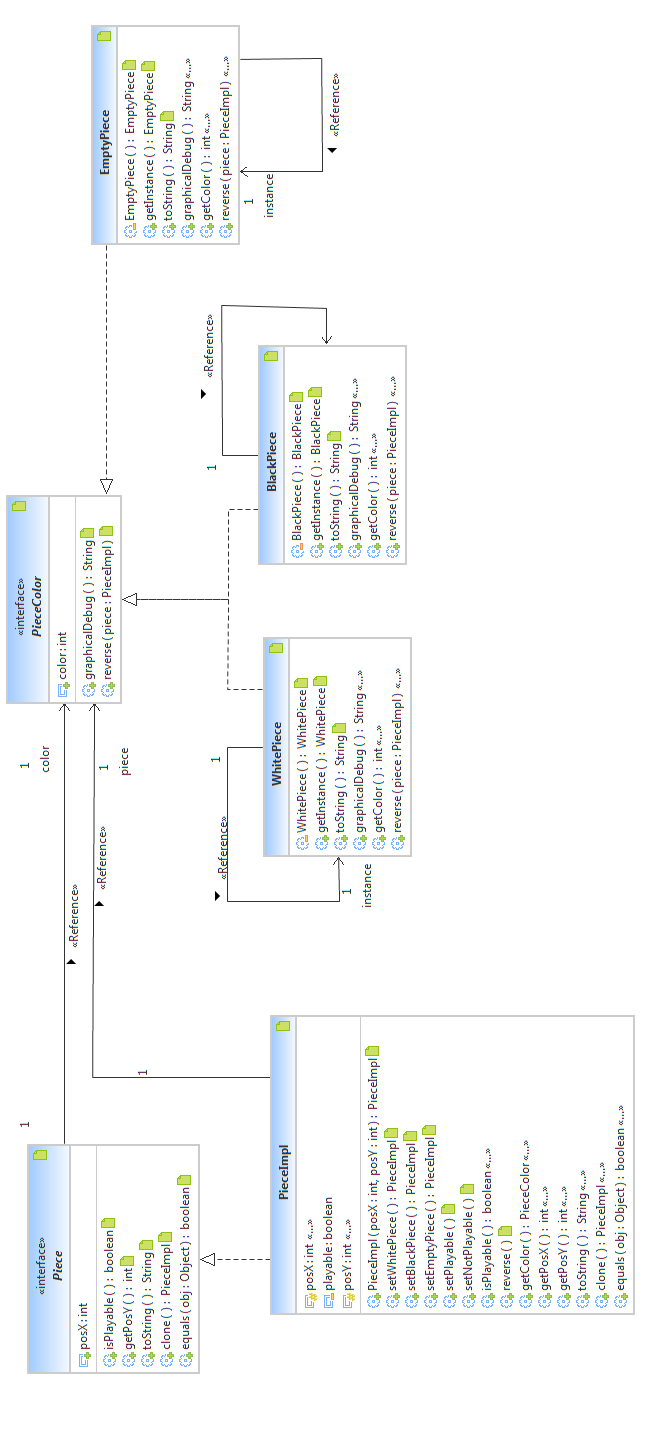
\includegraphics[scale=0.54]{Kernel/Pack_com_model_piece.png}
\caption{Diagramme UML de classes du Package Model.Piece du Logiciel}
\end{figure}

\label{OthKerModelView}
\begin{figure}[H]
\centering
 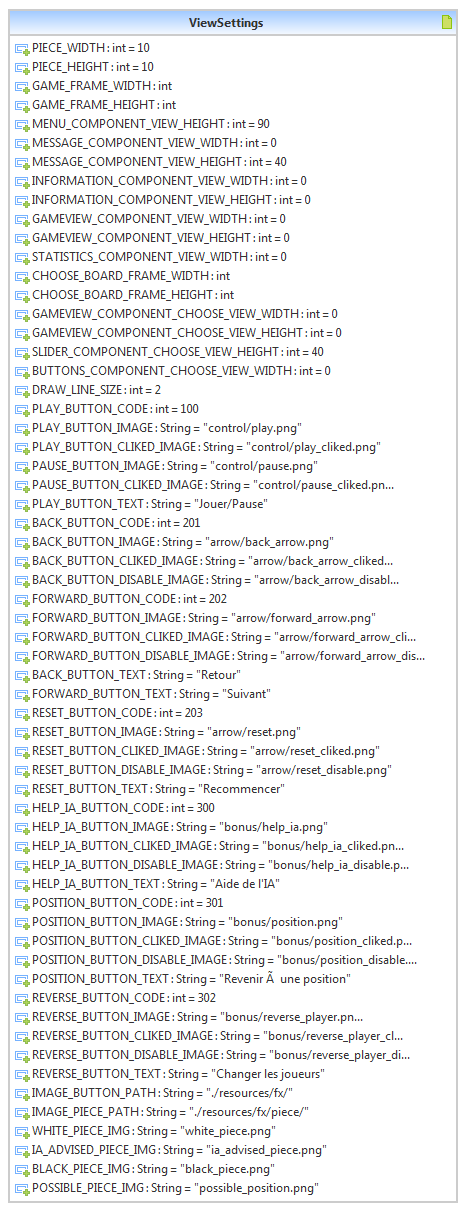
\includegraphics[scale=0.65]{Kernel/Pack_com_model_view.png}
\caption{Diagramme UML de classes du Package Model.View du Logiciel}
\end{figure}

\label{OthKerModelFactory}
\begin{figure}[H]
\centering
 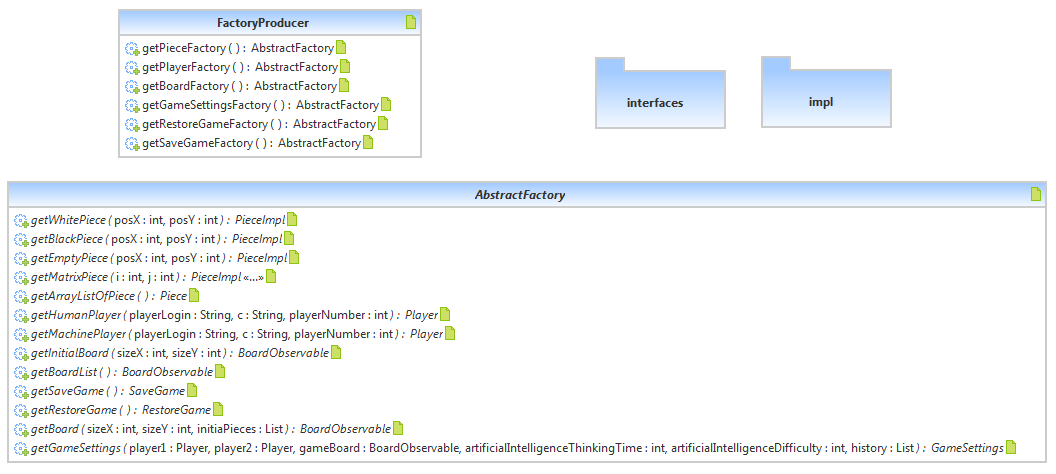
\includegraphics[scale=0.58]{Kernel/Pack_com_model_factory.png}
\caption{Diagramme UML de classes du Package Model.Factory du Logiciel}
\end{figure}

\label{OthKerModelFactoryInterfaces}
\begin{figure}[H]
\centering
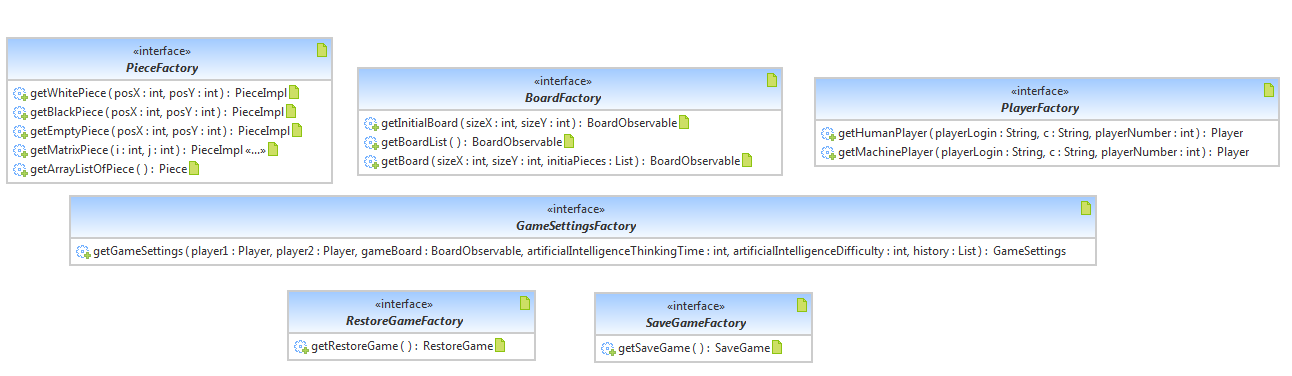
\includegraphics[scale=0.45]{Kernel/Pack_com_model_factory_interfaces.png}
\caption{Diagramme UML de classes du Package Model.Factory.Interfaces du Logiciel}
\end{figure}

\label{OthKerModelFactoryImpl}
\begin{figure}[H]
\centering
 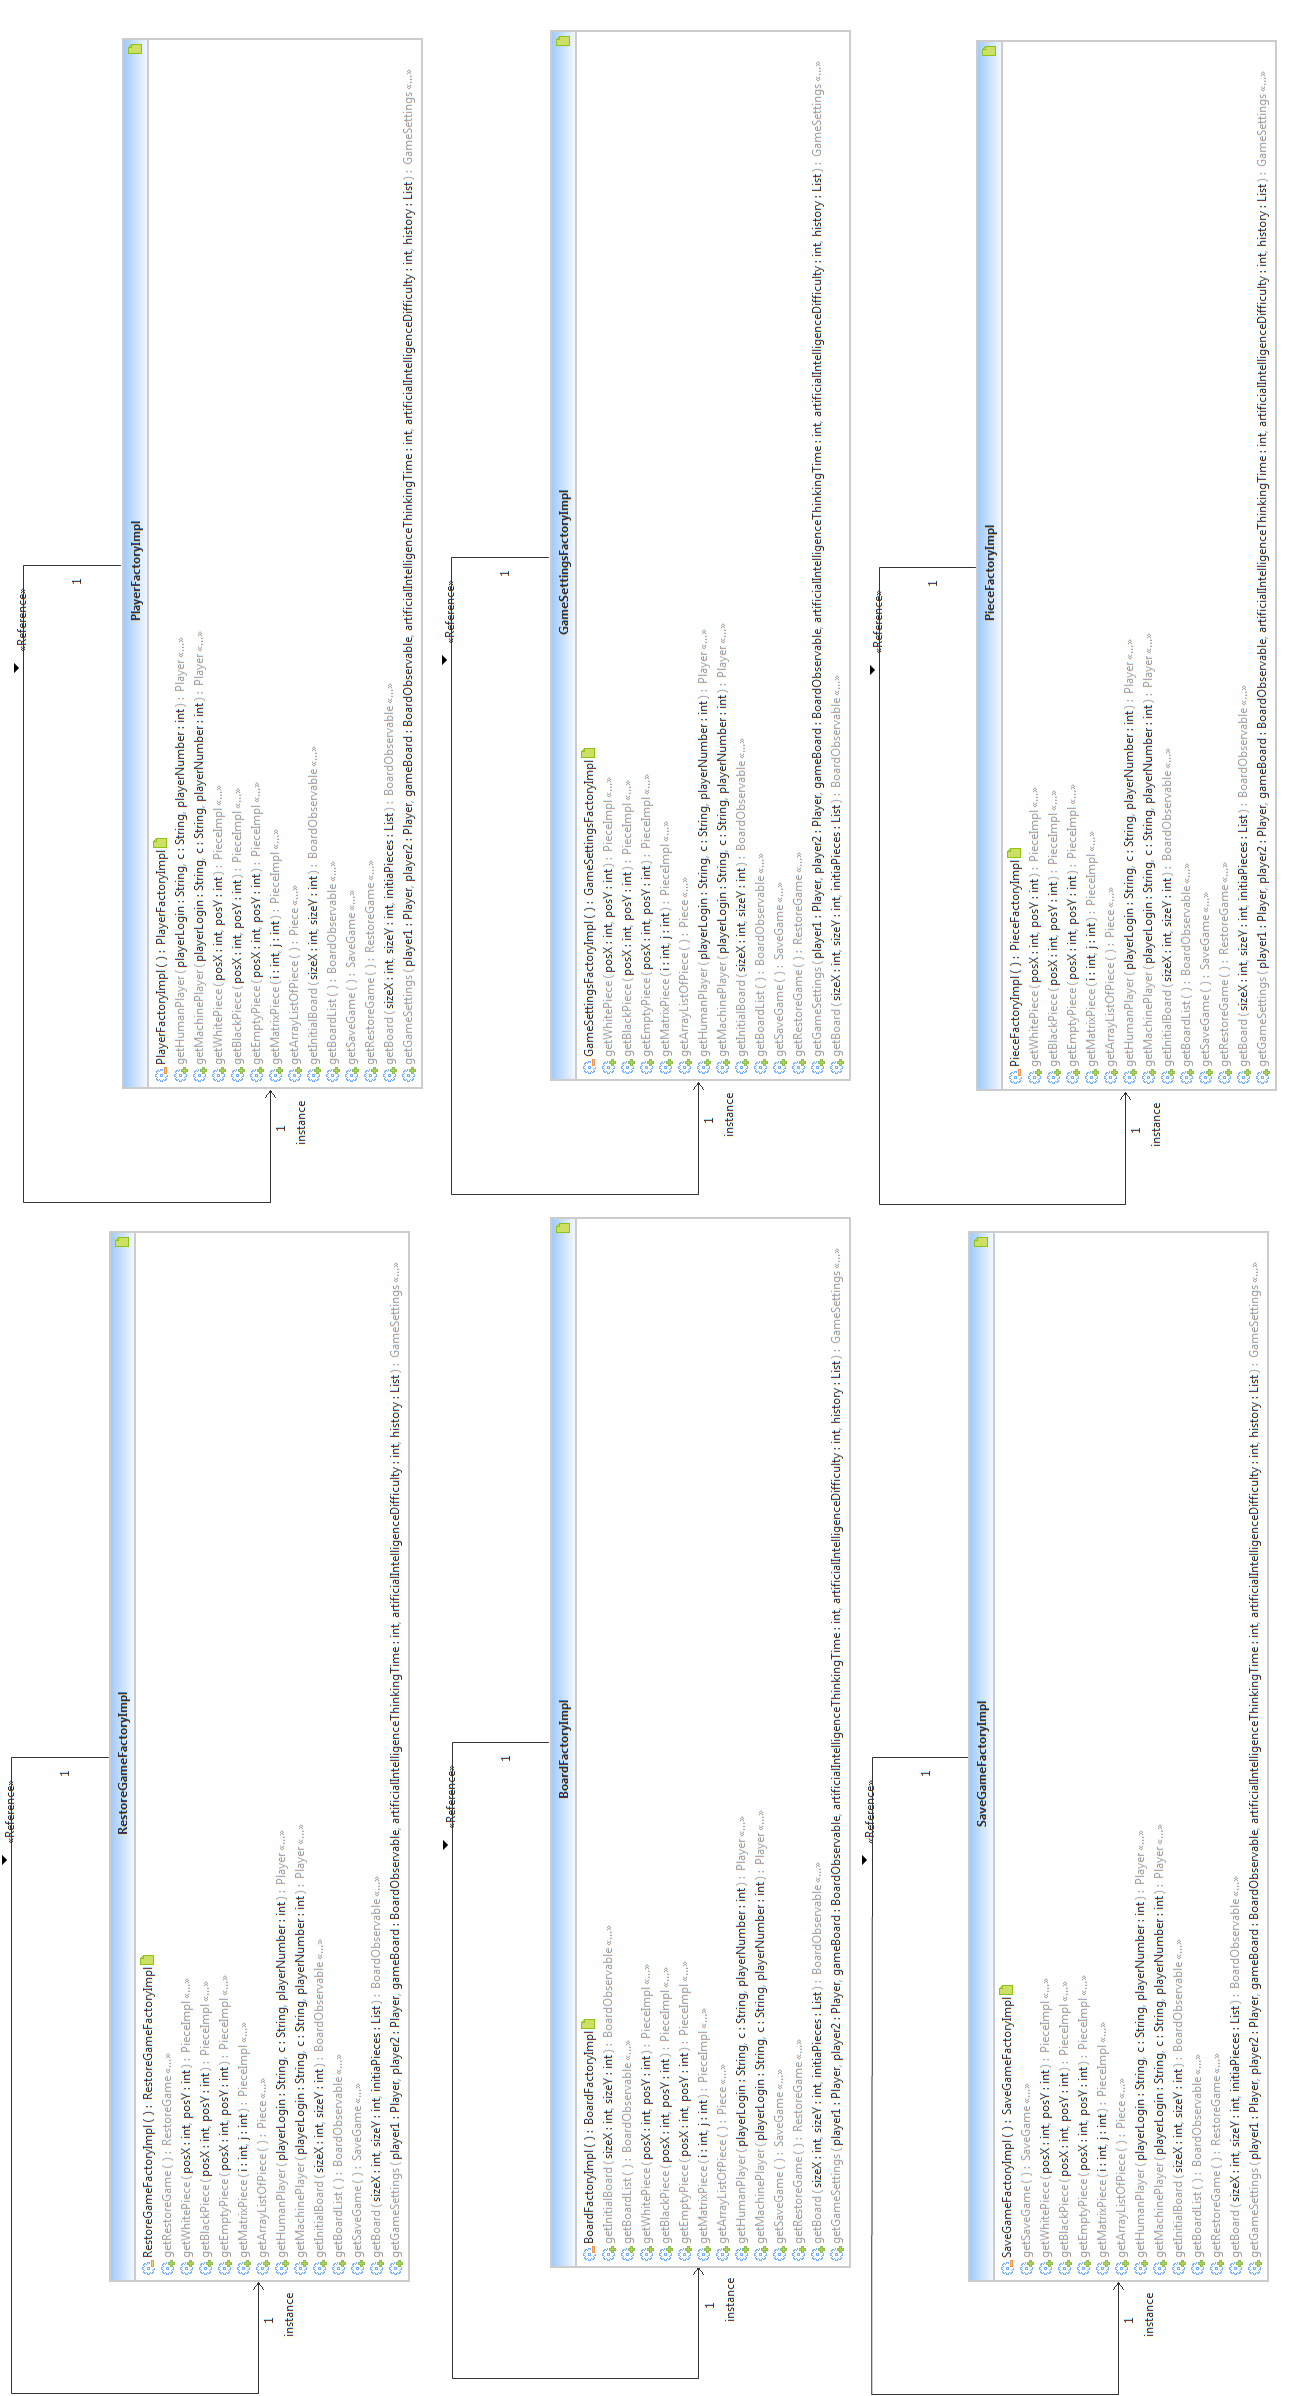
\includegraphics[scale=0.32]{Kernel/Pack_com_model_factory_impl.png}
\caption{Diagramme UML de classes du Package Model.Factory.Impl du Logiciel}
\end{figure}

\subsection{Vue du logiciel}
\label{OthKerView}
\begin{figure}[H]
\centering
 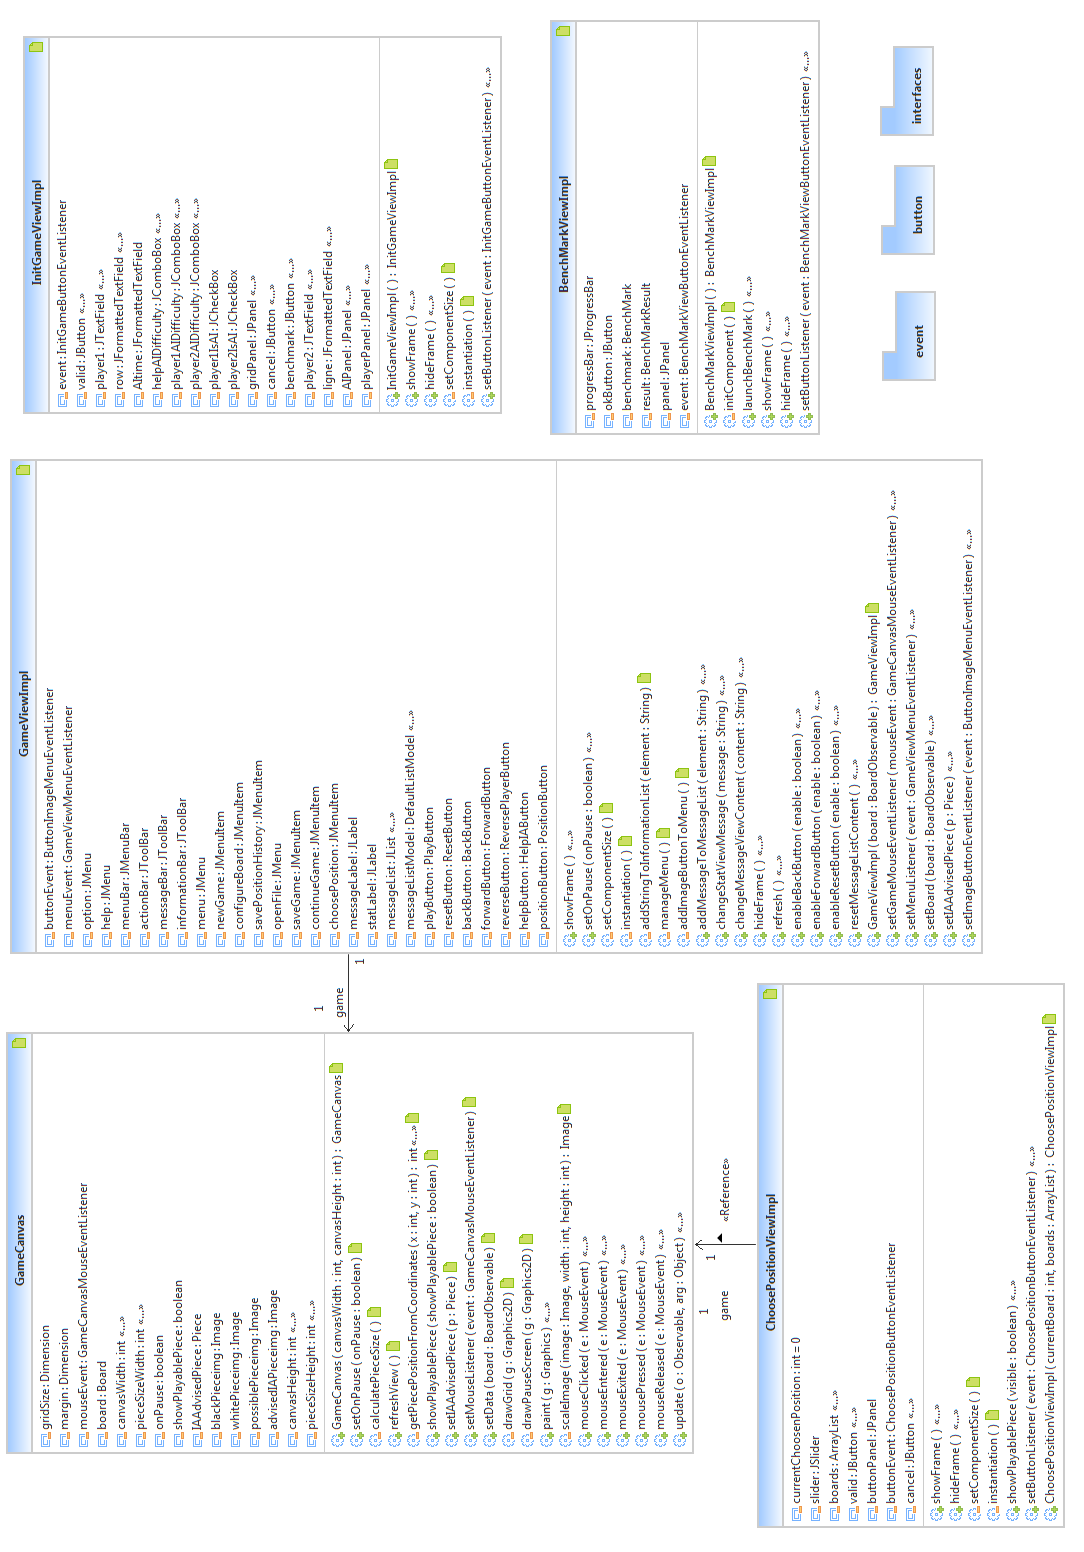
\includegraphics[scale=0.45]{Kernel/Pack_com_view.png}
\caption{Diagramme UML de classes du Package View du Logiciel}
\end{figure}

\label{OthKerViewInterfaces}
\begin{figure}[H]
\centering
 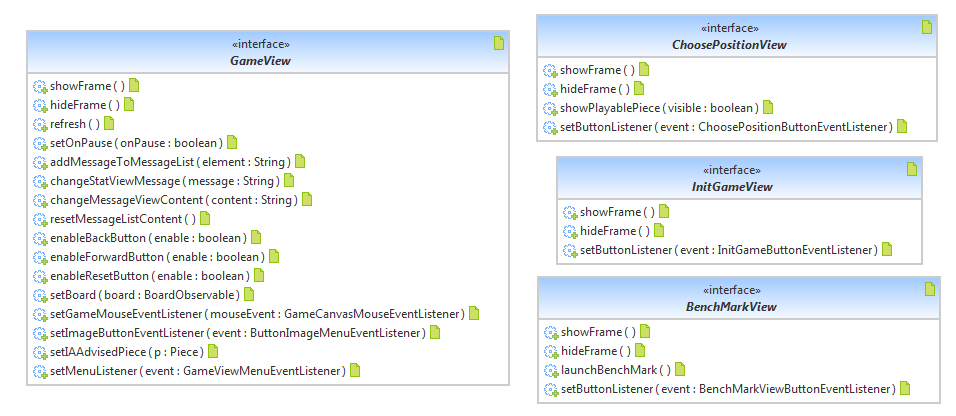
\includegraphics[scale=0.5]{Kernel/Pack_com_view_interfaces.png}
\caption{Diagramme UML de classes du Package View.Interfaces du Logiciel}
\end{figure}

\label{OthKerViewEvent}
\begin{figure}[H]
\centering
 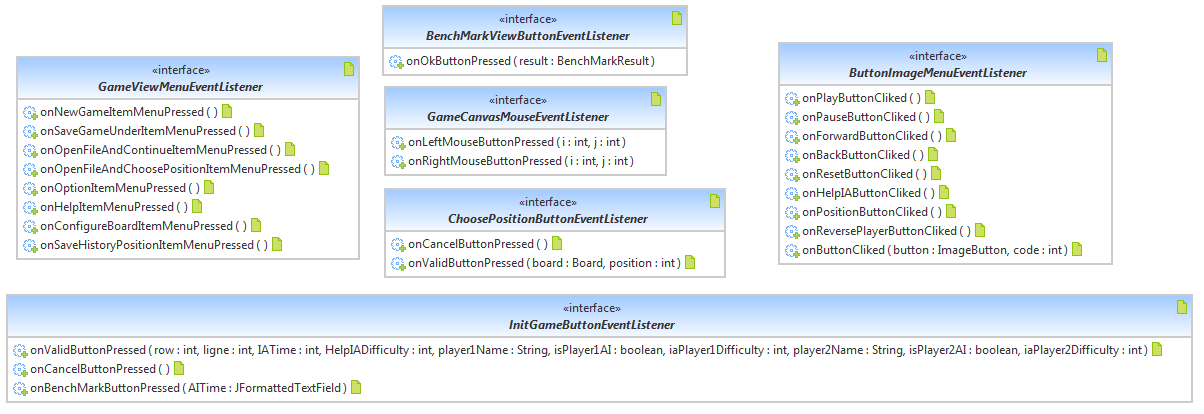
\includegraphics[scale=0.5]{Kernel/Pack_com_view_event.png}
\caption{Diagramme UML de classes du Package View.Event du Logiciel}
\end{figure}

\label{OthKerViewButton}
\begin{figure}[H]
\centering
  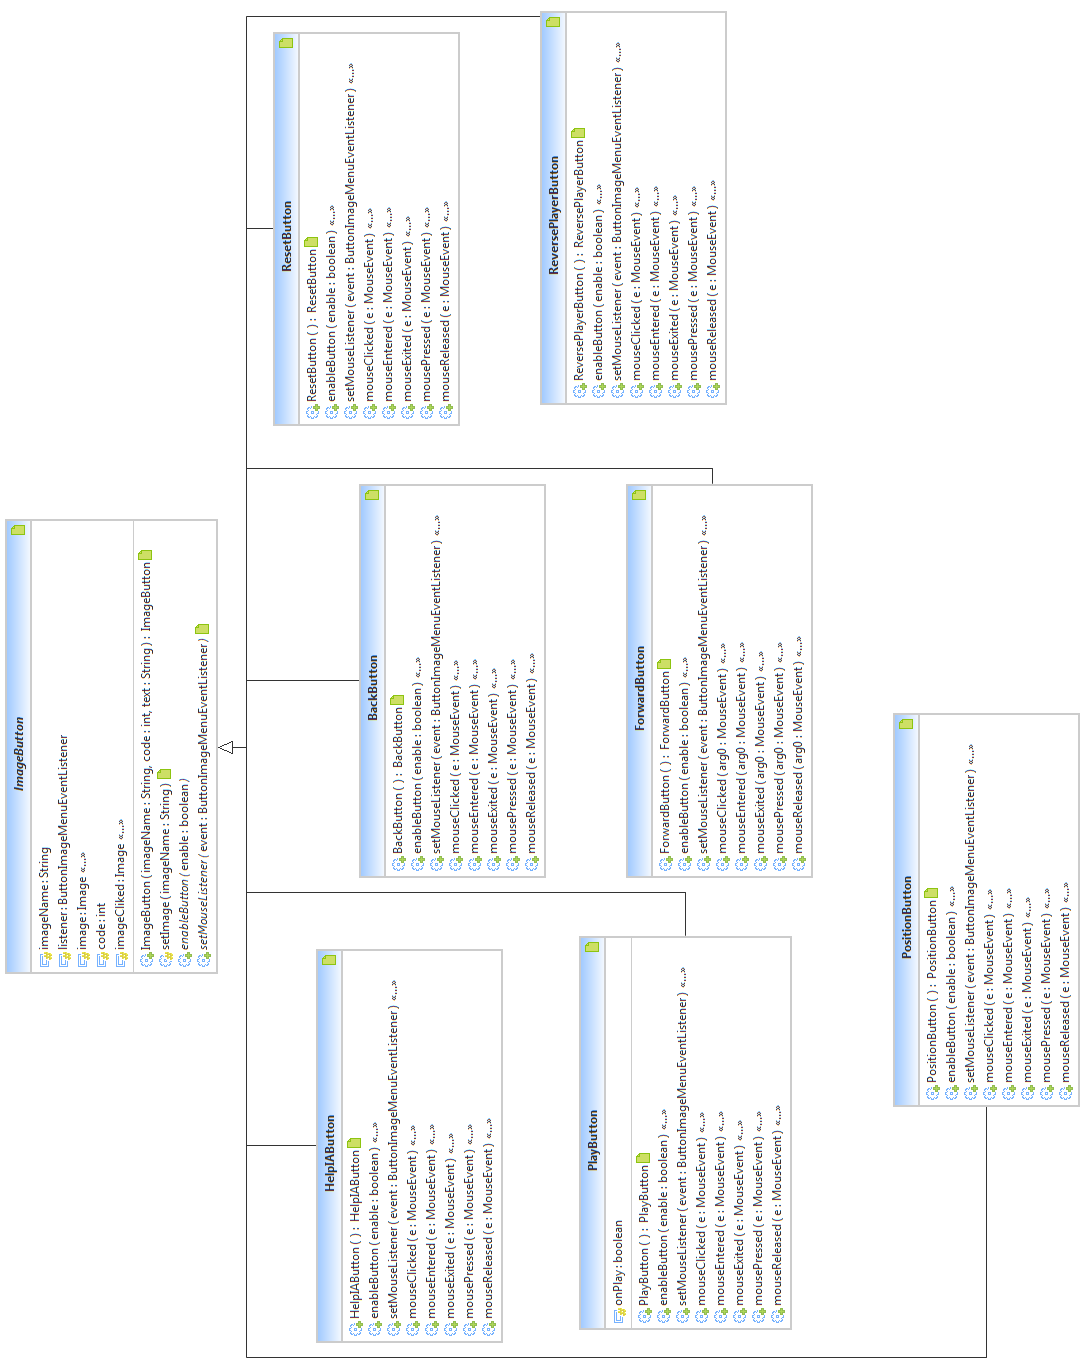
\includegraphics[scale=0.51]{Kernel/Pack_com_view_button.png}
\caption{Diagramme UML de classes du Package View.Button du Logiciel}
\end{figure}

\subsection{Contrôleur du logiciel}
\label{OthKerController}
\begin{figure}[H]
\centering
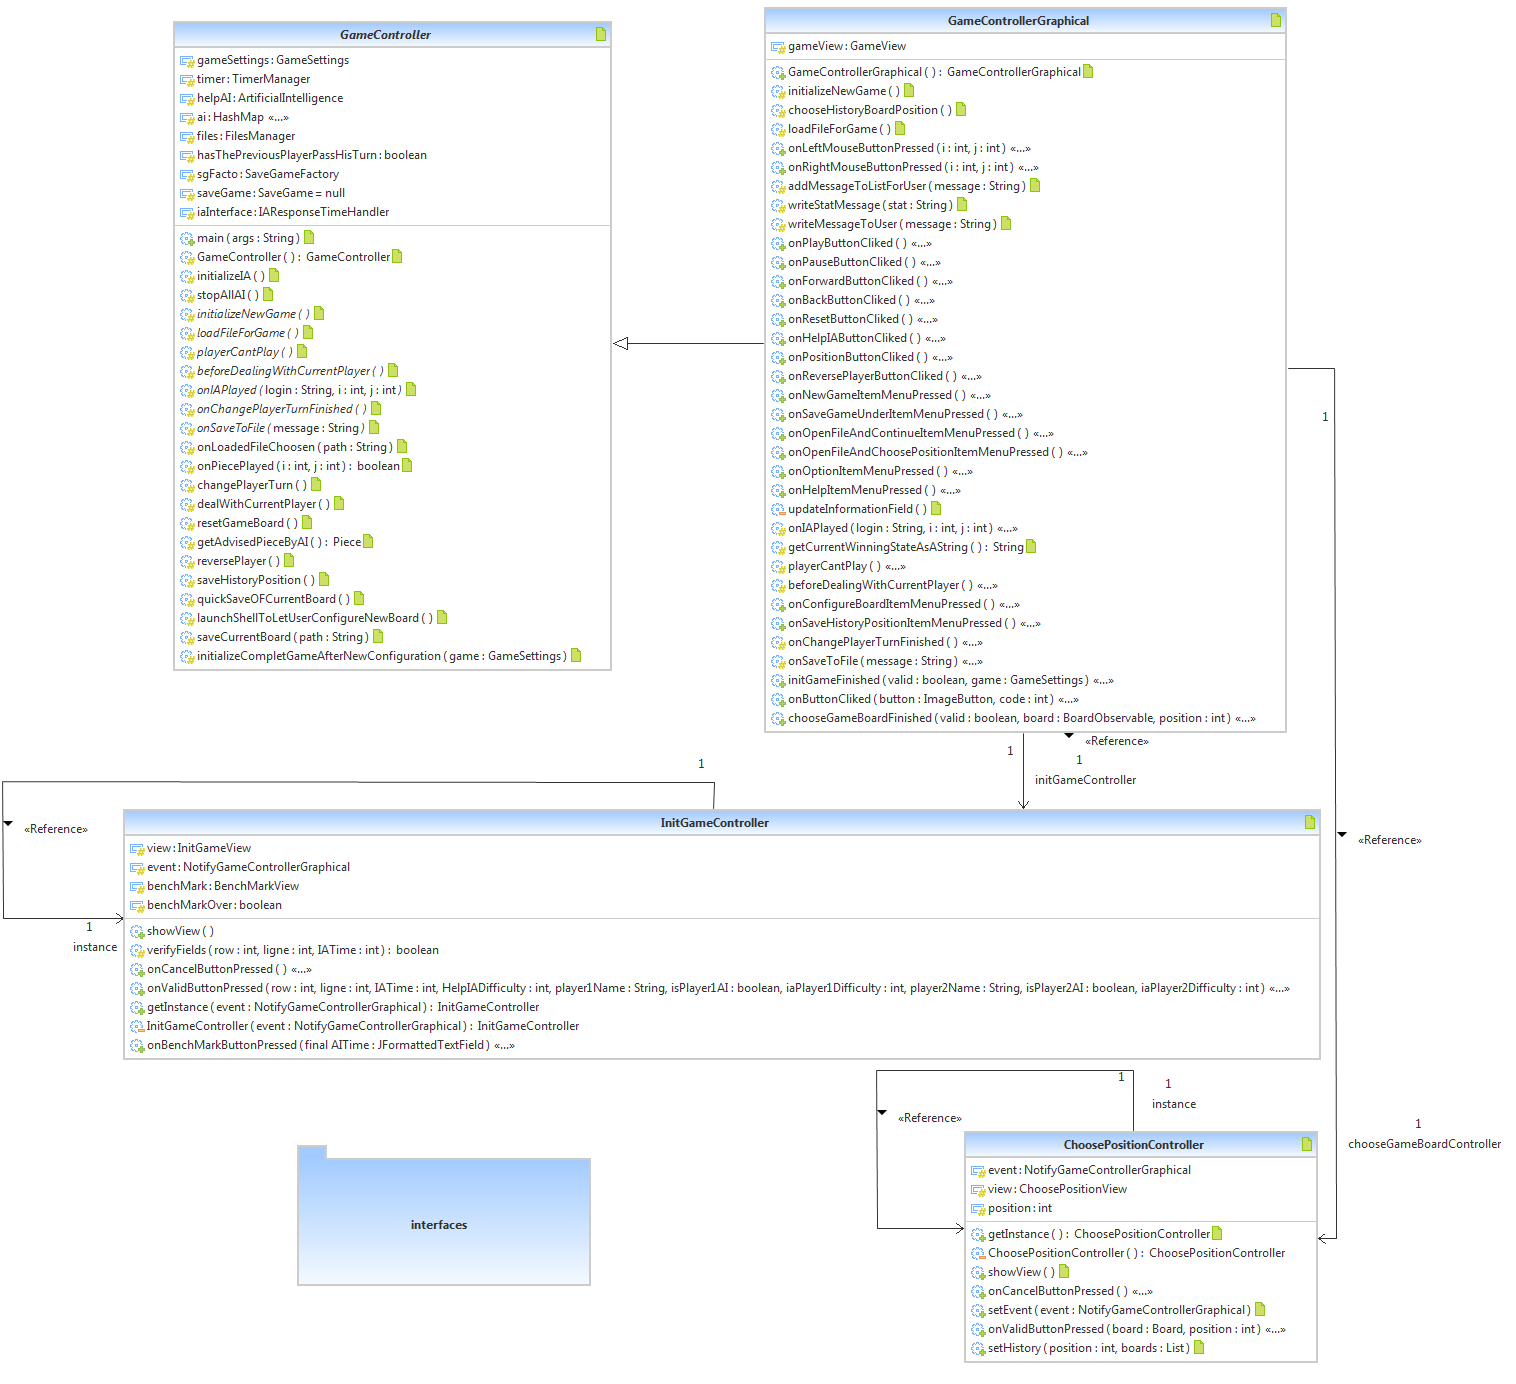
\includegraphics[scale=0.4]{Kernel/Pack_com_controller.png}
\caption{Diagramme UML de classes du Package Controller du Logiciel}
\end{figure}


\label{OthKerControllerInterfaces}
\begin{figure}[H]
\centering
 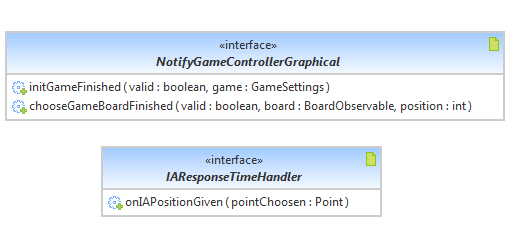
\includegraphics[scale=1.0]{Kernel/Pack_com_controller_interfaces.png}
\caption{Diagramme UML de classes du Package Controller.Interfaces du Logiciel}
\end{figure}

\subsection{Utils du logiciel}
\label{OthKerUtils}
\begin{figure}[H]
\centering
 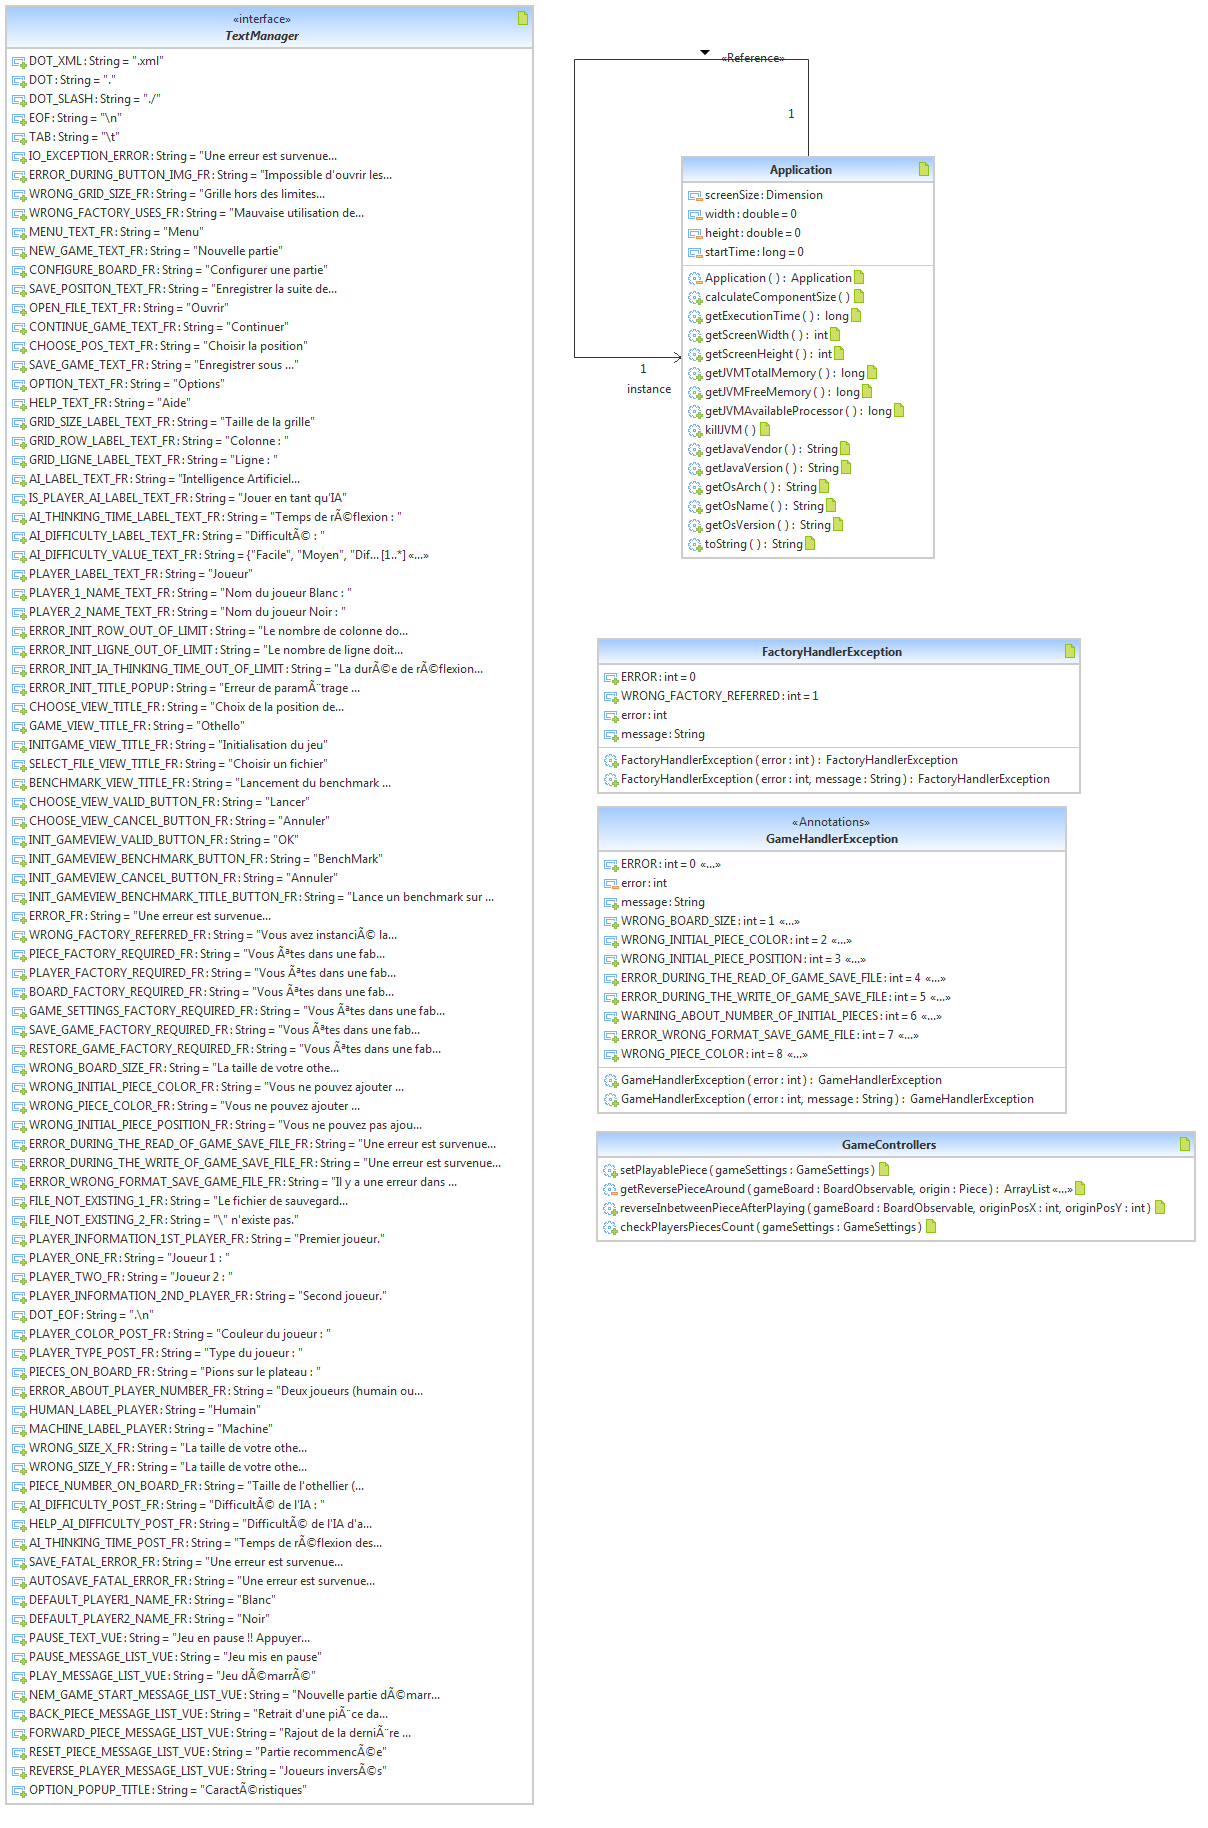
\includegraphics[scale=0.35]{Kernel/Pack_utils.png}
\caption{Diagramme UML de classes du Package Utils du Logiciel}
\end{figure}

\section{Diagramme de classes Intelligence Artificielle}
\label{clsAI}
\begin{figure}[H]
\centering
  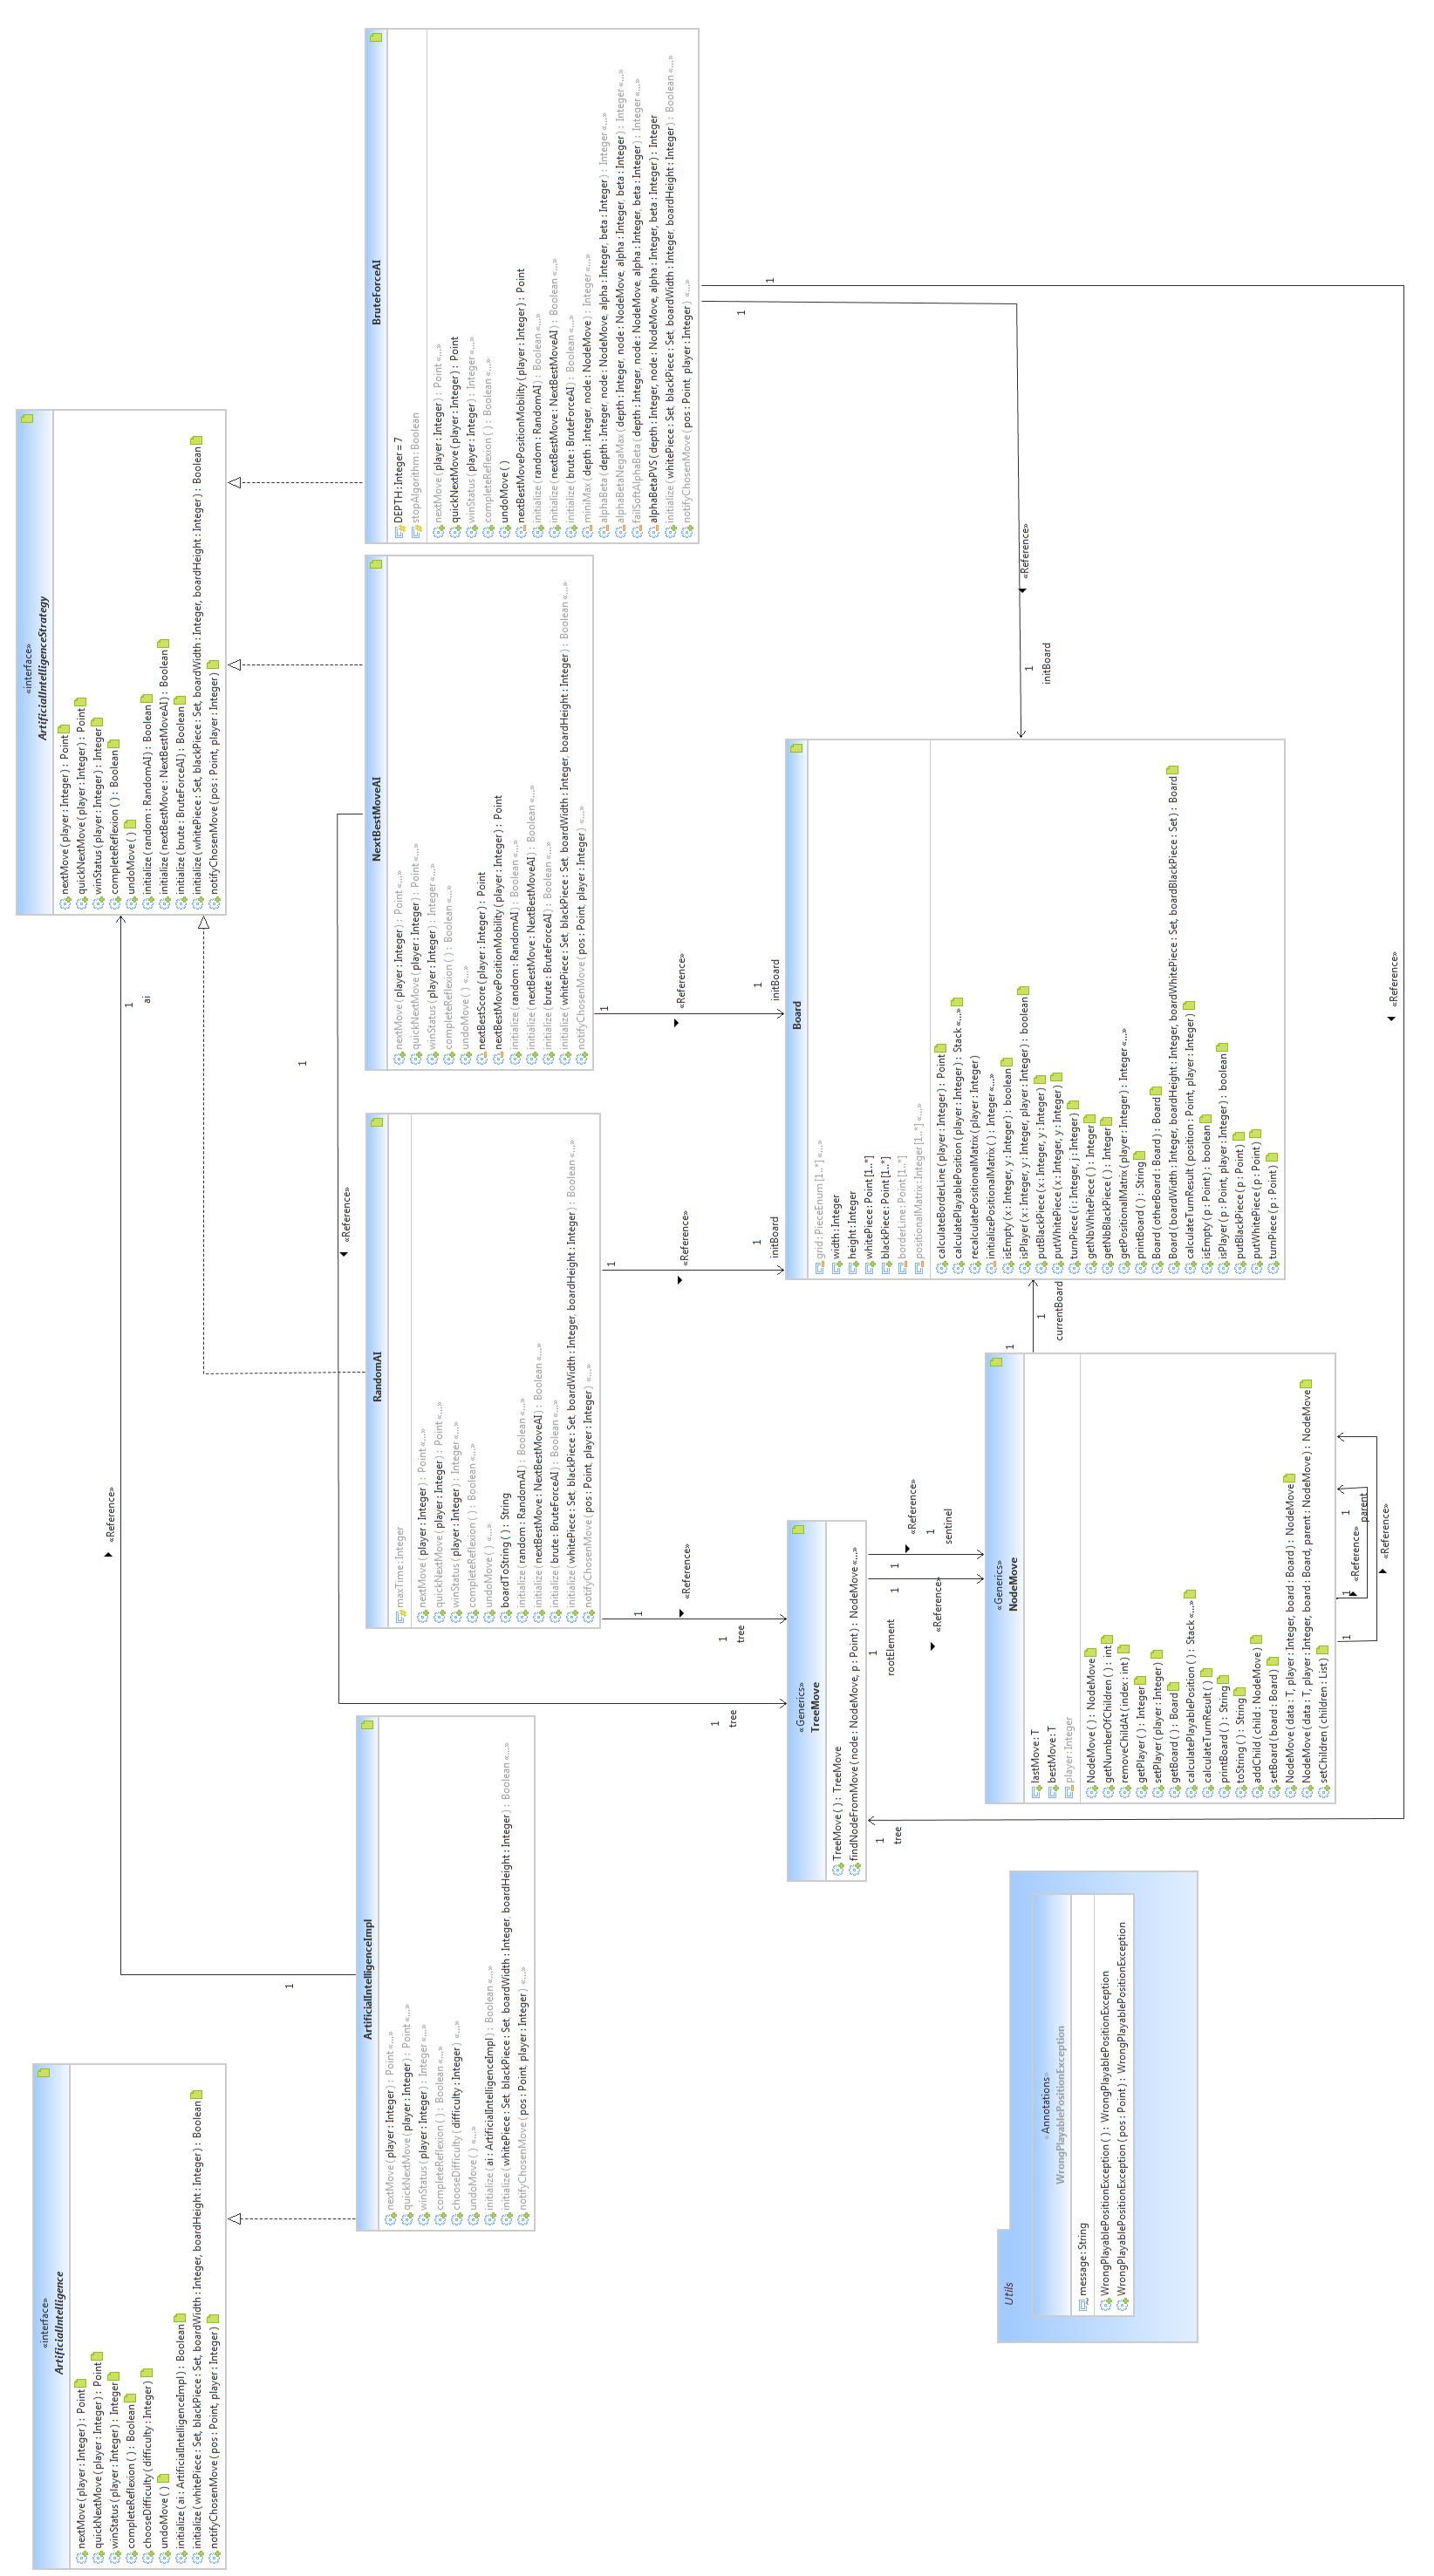
\includegraphics[scale=0.23]{Architecture/ArtificialIntelligence.png}
\caption{Diagramme UML de classes de l'intelligence Artificielle}
\end{figure}

\section{Diagramme de classes du gestionnaire de fichiers}
\label{clsFM}
\begin{figure}[H]
\centering
  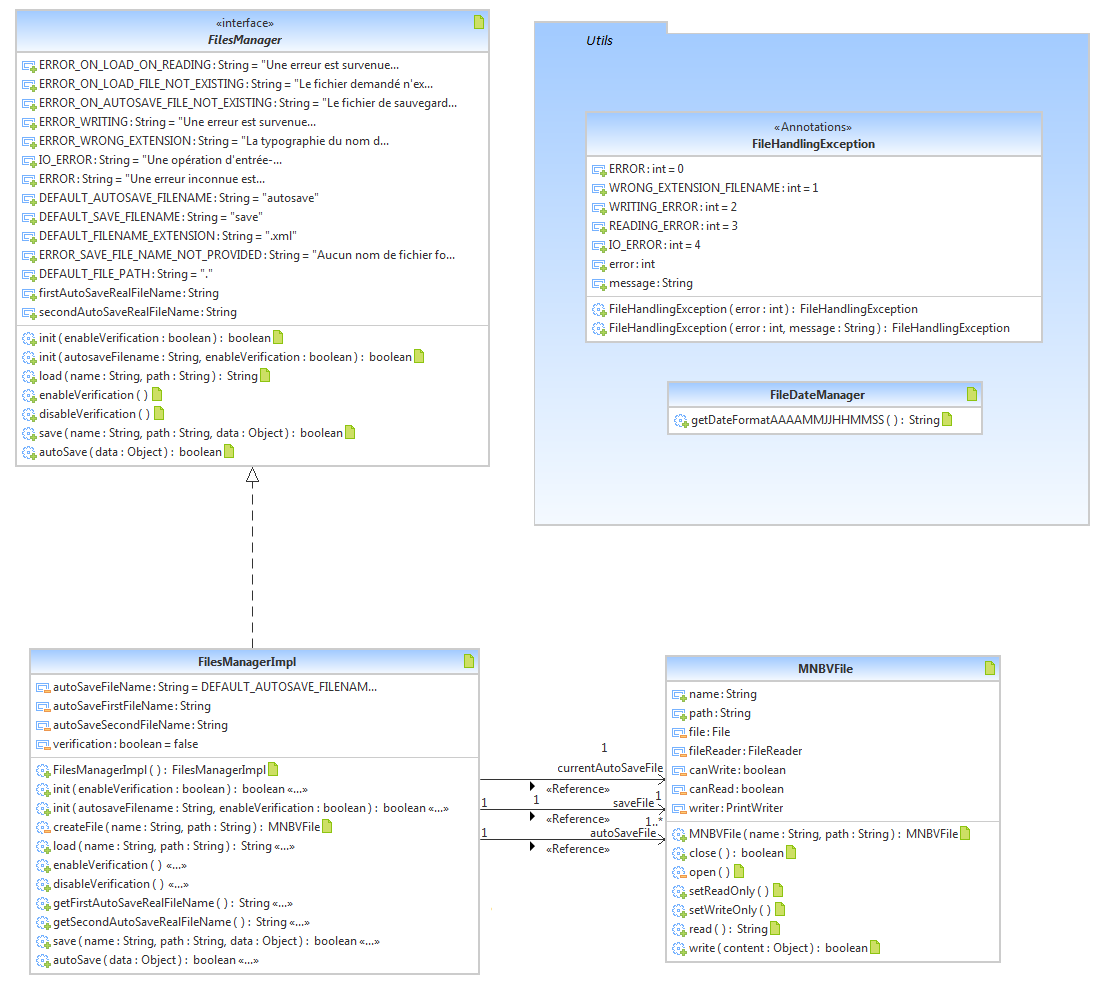
\includegraphics[scale=0.5]{Architecture/FilesManager.png}
\caption{Diagramme UML de classes du Gestionnaire de fichiers}
\end{figure}

\section{Diagramme de classes de l'Editeur de plateaux}
\label{clsBP}
\begin{figure}[H]
\centering
  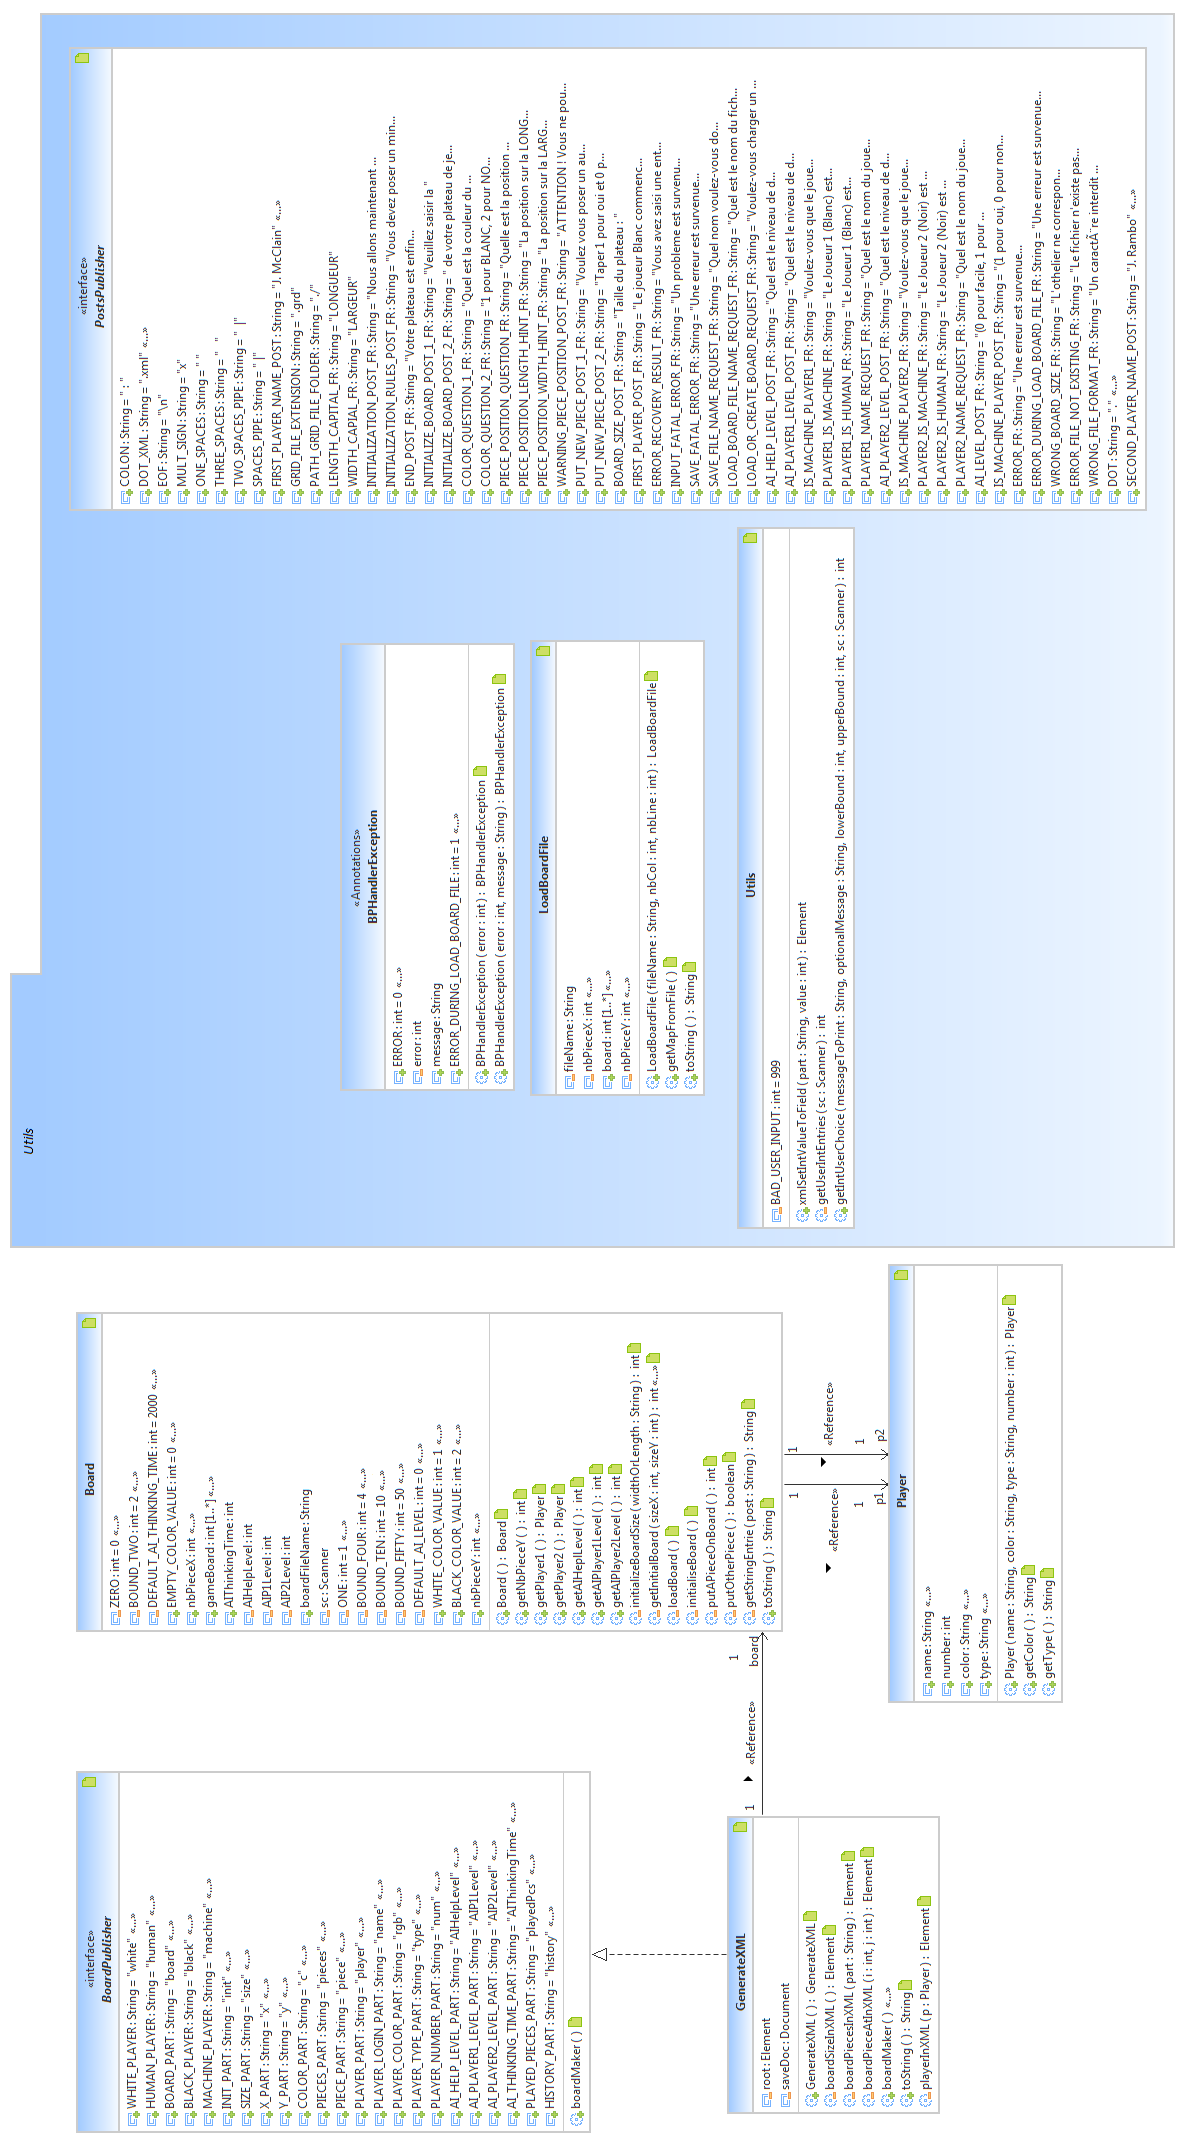
\includegraphics[scale=0.34]{Architecture/BoardPublisher.png}
\caption{Diagramme UML de classes de l'Editeur de plateaux}
\end{figure}

\section{Diagramme de classes du Gestionnaire de temps}
\label{clsT}
\begin{figure}[H]
\centering
  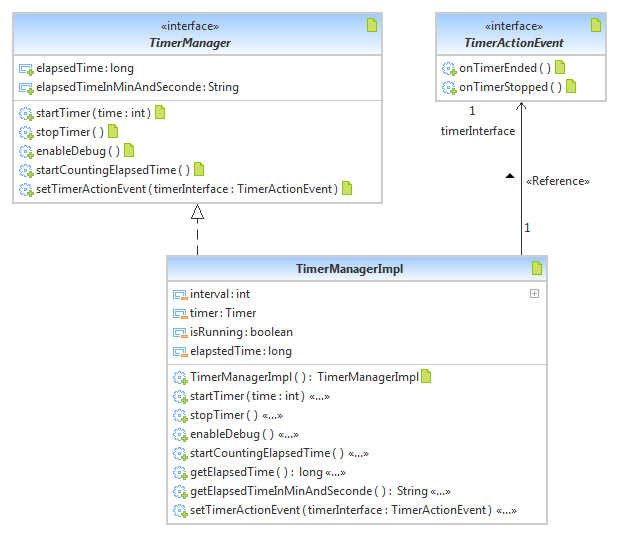
\includegraphics[scale=0.8]{Architecture/PdpTimer.png}
\caption{Diagramme UML de classes du Gestionaire de temps}
\end{figure}

\chapter{Pseudo-codes d'algorithmes}
\lstset{language=C++,basicstyle=\ttfamily\scriptsize}     
\section{Algorithme MiniMax}
\begin{figure}[H]
\begin{lstlisting}[frame=single]
int fonction minimax (int depth){
   if (game over or depth = 0)
      return winning score or eval();
   int bestScore;
   move bestMove;
   if (noeud == MAX) { //=Programme
      bestScore = -INFINITY;
      for (each possible move m) {
         make move m;
         int score = minimax (depth - 1)
         unmake move m;
         if (score > bestScore) {
            bestScore = score;
            bestMove = m ;
         }
      }
   }
   else { //type MIN = adversaire
      bestScore = +INFINITY;
      for (each possible move m) {
         make move m;
         int score = minimax (depth - 1)
         unmake move m;
         if (score < bestScore) {
            bestScore = score;
            bestMove = m ;
         }
      }
   }
   return bestscore ;
}
\end{lstlisting}
\caption{Pseudo-code de l'algorithme MiniMax \cite{1}}
\label{codemin}
\end{figure}

\lstset{language=C++,basicstyle=\ttfamily\footnotesize}     
\section{Algorithme Alpha-Beta}
\begin{figure}[H]
\begin{lstlisting}[frame=single]
int alphabeta(int depth, int alpha, int beta)
{
   if (game over or depth <= 0)
      return winning score or eval();
   move bestMove;
   if(noeud == MAX) { //Programme
      for (each possible move m) {
         make move m;
         int score = alphabeta(depth - 1, alpha, beta)
         unmake move m;
         if (score > alpha) {
            alpha = score;
            bestMove = m ;
            if (alpha >= beta)
               break;
         }
      }
      return alpha ;
   } 
   else { //type MIN = adversaire
      for (each possible move m) {
         make move m;
         int score = alphabeta(depth - 1, alpha, beta)
         unmake move m;
         if (score < beta) {
            beta = score;
            bestMove = m ;
            if (alpha >= beta)
               break;
         }
      }
      return beta;
   }
}
\end{lstlisting}
\caption{Pseudo-code de l'algorithme Alpha-Beta \cite{1}}
\label{codealpha}
\end{figure}

\chapter{Site Web}

Nous avons choisi de développer un site web en local pour plusieurs raisons. La principale raison est qu’il nous sert de support pour l’aide du jeu. Il nous permet également de présenter le projet, l’équipe et d’avoir accès à la documentation.

\begin{figure}[H]
\centering
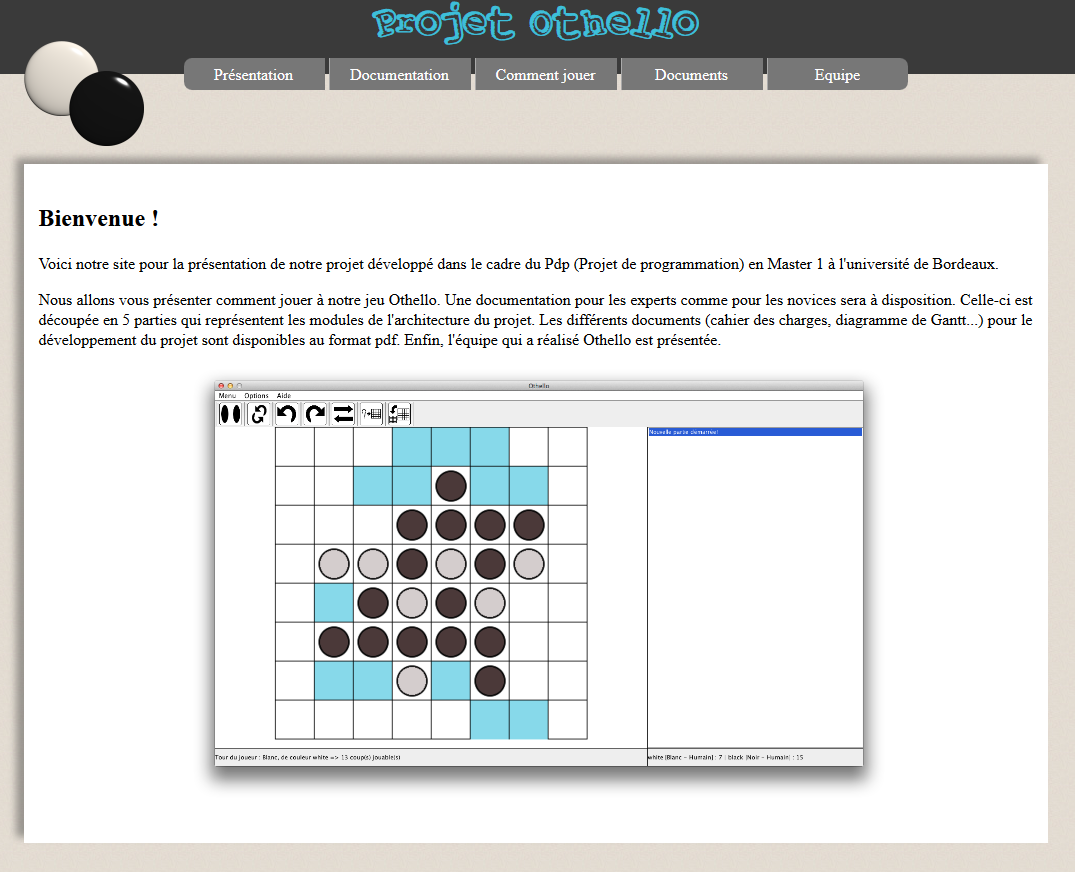
\includegraphics[scale=0.39]{Images/capture_site.png}
\caption{Capture du site internet}
\label{site}
\end{figure}

\centerline{\url{http://morgane.badre.1.emi.u-bordeaux1.fr/Othello/}}

\chapter{Poster}

Nous avons eu l’opportunité dans le cadre du cours de communication de réaliser un poster. C’était un moyen d’agrémenter et de présenter notre projet.

\begin{figure}[H]
\centering
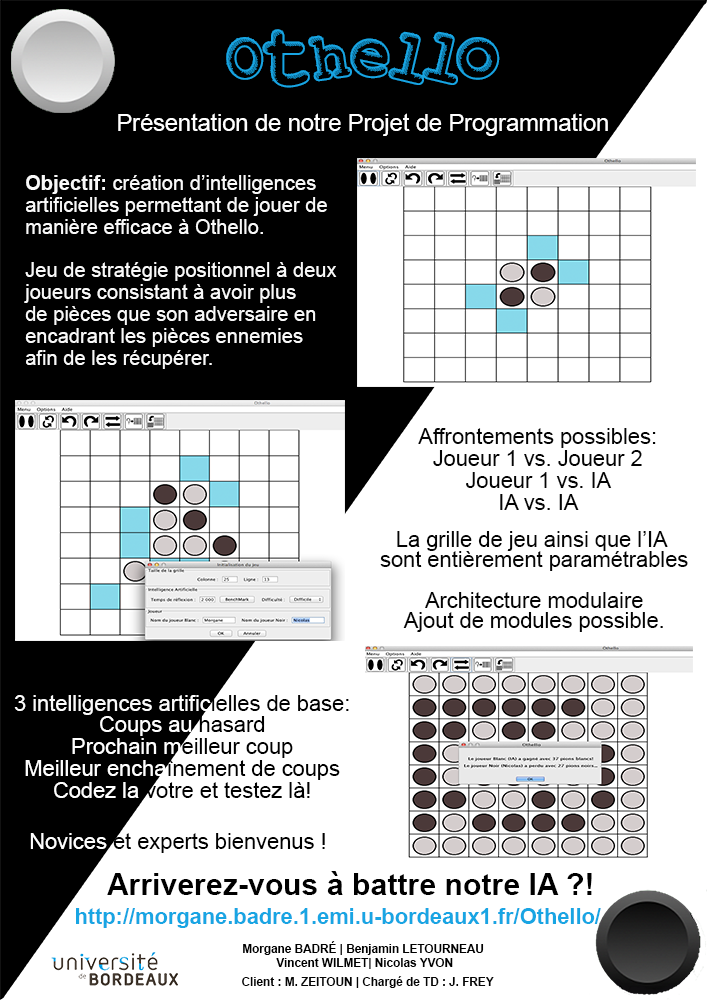
\includegraphics[scale=1.5]{Images/posterfinal.png}
\caption{Poster du projet}
\label{poster}
\end{figure}

\end{document}


